\documentclass{fhnwreport/fhnwreport}


\usepackage{lipsum}
\usepackage[ngerman]{babel}
\usepackage[T1]{fontenc}
\usepackage[utf8x]{inputenc}
\usepackage{tikz}
\usepackage{amsmath}
\usepackage{amsfonts}
%\usepackage{MnSymbol}
\usepackage{wasysym}
\usetikzlibrary{arrows}
\usepackage{lmodern}   %Type1-Schriftart f\"ur nicht-englische Texte
\usepackage{datetime}
\usepackage{cite}
\usepackage{lipsum}
\usepackage{booktabs}
\usepackage{pdflscape}
\usepackage{longtable}
\usepackage{rotating}
\usepackage{xcolor}
\usepackage{colortbl}
\usepackage{hyperref}
\usepackage{appendix}
\usepackage{graphicx}
\usepackage{pdfpages}
\usepackage{enumitem}
\usepackage{caption}
\usepackage{gensymb}
\usepackage{pbox}
%\usepackage{draftwatermark}
%\usepackage[nostamp]{draftwatermark}
\usepackage[textsize=footnotesize, textwidth = 17mm, german, colorinlistoftodos]{todonotes}
\usepackage{siunitx}
\usepackage{mathtools}
\usepackage{matlab-prettifier}

\definecolor{dkgreen}{rgb}{0,0.6,0}
\definecolor{gray}{rgb}{0.5,0.5,0.5}
\definecolor{mauve}{rgb}{0.58,0,0.82}

\lstdefinestyle{java}{
    language            = Java,
    aboveskip           = 3mm,
    belowskip           = 3mm,
    showstringspaces    = false,
    columns             = flexible,
    basicstyle          = {\scriptsize\ttfamily},
    numbers             = left,
    numberstyle         = \tiny\color{gray},
    keywordstyle        = \color{blue},
    commentstyle        = \color{dkgreen},
    stringstyle         = \color{mauve},
    breaklines          = true,
    breakatwhitespace   = true,
    tabsize             = 3
}
\lstdefinestyle{Matlab-editor-2}{%
  style               = MatlabBaseStyle@mlpr,
  mllastelementstyle  = \color{black}                    ,
  mlkeywordstyle      = \color[RGB]{000,000,255}         ,
  mlcommentstyle      = \color[RGB]{034,139,034}         ,
  mlstringstyle       = \color[RGB]{160,032,240}         ,
  mlsyscomstyle       = \color[RGB]{178,140,000}         ,
  mlsectiontitlestyle = \commentStyle@mlpr      \bfseries,
  mlsharedvarstyle    = \color[RGB]{000,163,163}         ,
  mlplaceholderstyle  = \mleditorphstyle,
  basicstyle          = \ttfamily\scriptsize,
  numbers             = left,
}


%\SetWatermarkText{\texttt{Entwurf}}
%\SetWatermarkText{Entwurf}
%\SetWatermarkLightness{0.9}

\setcounter{secnumdepth}{5}
\setcounter{tocdepth}{2}

\DeclarePairedDelimiter\abs{\lvert}{\rvert}%

\renewcommand{\thesubsubsection}{\arabic{subsubsection}}

%\renewcommand{\thefootnote}{\roman{footnote}}
\renewcommand{\thefootnote}{\Roman{footnote}}

\hypersetup{%
  bookmarksnumbered = true,
  colorlinks = true,
  linkcolor  = black,
  citecolor  = black,
  %urlcolor   = blue,
  urlcolor   = black,
  %hidelinks  = false
}

\title{%
    \textbf{\Huge{Laborjournal}} \\
    \date{\vspace{-5ex}}
}

\newcommand{\colfigure}[3]{%
    \begin{minipage}[c][][b]{0.485\textwidth}
        #1
    \end{minipage}
    \hspace{0.03\textwidth}
    \begin{minipage}[c][][b]{0.485\textwidth}
        {\raggedleft%
            \includegraphics[width=0.9\textwidth]{#2}%
        }
        \captionof{figure}{#3}
    \end{minipage}\\%
}

\newlist{longenum}{enumerate}{5}
\setlist[longenum,1]{label=\roman*)}
\setlist[longenum,2]{label=\alph*)}
\setlist[longenum,3]{label=\arabic*)}
\setlist[longenum,4]{label=(\roman*)}
\setlist[longenum,5]{label=(\alph*)}

\def\code#1{\texttt{#1}}
\def\quelleVA{\emph{Quelle:} Versuchsanleitung}

\DeclareSIUnit[number-unit-product = {}]
    \partspermillion{ppm}
\DeclareSIUnit[number-unit-product = {}]
    \permille{\perthousand}

\newenvironment{conditions}
  {\noindent Wobei: \par\vspace{\abovedisplayskip}\noindent\begin{tabular}{>{$}l<{$} @{${}:{}$} l}}
  {\end{tabular}\par\vspace{\belowdisplayskip}}



\begin{document}

\begin{titlepage}

    \maketitle

    \vspace{10mm}
    \begin{center}
    \begin{tabular}{lr}

        \Huge{Versuchsleiter:} & \Huge{Raphael Frey} \\
        \Huge{Assistent:} & \Huge{Mario H\"asler} \\

    \end{tabular}

    \vspace{20mm}

    %\hspace{-20mm}
    \Large
    \begin{tabular}{p{27mm}|p{67mm}|p{23mm}|p{26mm}}

        %\textsc{\textbf{Autoren}}
        %& Anita Rosenberger, Benjamin M\"uller, Manuel Suter, Florian Alber, Raphael Frey\\
        %[4mm]

        \textsc{Datum Durchf\"uhrung} & \textsc{Versuch} & \textsc{Datum Abgabe} & \textsc{Akzeptiert, Note} \\
        [10mm]
        \hline
        25.02.2016 & W4b -- Kombipendel                     & 24.03.2016 & \\
        [10mm]
        24.03.2016 & A11 -- R\"ontgenstrahlung/-beugung     & 14.04.2016 & \\
        [10mm]
        28.04.2016 & O12 -- Laser Doppler Anemometrie       & 26.05.2016 & \\

    \end{tabular}
    \end{center}
    \normalsize

\end{titlepage}


% **************************************************************************** %
\clearpage
\pagestyle{empty}
{
    \renewcommand{\thispagestyle}[1]{}
    \newgeometry{bottom=20mm}

    % ************************************************************************ %
    %\section*{Grundidee}
    %\label{sec:grundidee}
    % ************************************************************************ %
    %\input{sections/grundidee.tex}


    \clearpage
    \tableofcontents
    %\vspace{5mm}
    \subsubsection*{Versionsgeschichte}
    \small{
        \begin{itemize}
            \item[]
                \emph{27.04.2016:} \texttt{Version 0.1}: Vorbereitung
            \item[]
                \emph{01.05.2016:} \texttt{Version 0.2}: Arbeitsgrundlagen, Durchf\"uhrung, Auswertung tlw.
            \item[]
                \emph{02.05.2016:} \texttt{Version 0.3}: Fix Auswertung, Fehlerrechnung, Diskussion
            \item[]
                \emph{03.05.2016:} \texttt{Version 0.4}: Formatierung, Erg\"anzung bei Messung Rohrmitte
            \item[]
                \emph{04.05.2016:} \texttt{Version 1.0}
        \end{itemize}
    }
    \restoregeometry
}

\clearpage
\setcounter{page}{1}
\pagestyle{headings}
% **************************************************************************** %


% **************************************************************************** %
\clearpage
\section{Arbeitsgrundlagen}
\label{sec:arbeitsgrundlagen}
% **************************************************************************** %
In  diesem  Versuch kommen  verschiedene  Bereiche  aus der  Physik  zusammen,
prim\"ar Fluid-Dynamik und Optik. Entsprechend ergibt sich auch die Gliederung
dieses Kapitels.

% ---------------------------------------------------------------------------- %
\subsection{Messprinzip}
\label{subsec:messprinzip}
% ---------------------------------------------------------------------------- %

Das Verfahren nutzt den optischen  Dopplereffekt, um die Geschwindigkeit eines
Teilchens in einem  Fluid zu detektieren. Trifft ein  Lichtstrahl der Frequenz
$f$ auf  ein bewegtes Objekt,  unterschheidet sich die vom  Objekt detektierte
Frequenz $f_1$ ein wenig von der vom Sender emittierten Frequenz $f_0$.

\begin{equation}
    \label{eq:doppler}
    f_1 = f_0 \cdot \left( 1 - \frac{\vec{e} \cdot \vec{v}}{c} \right)
        = f_0 \cdot \left( 1 + \frac{v}{c} \cdot \cos{\vartheta_1} \right)
\end{equation}

Wobei $c$  die Lichtgeschwindigkeit, $\vec{e}$ ein  Einheitsvektor in Richtung
des  Lichtstrahls  und  $\vec{v}$   der  Geschwindigkeitsvektor  des  bewegten
Objektes ist. Wird der Lichtstrahl am bewegten Objekt gestreut und anschliessend
von einem Empf\"anger detektiert, ergibt sich f\"ur diesen die Frequenz $f_2$:

\begin{equation}
    \label{eq:doppler:gestreut}
    f_2
        = f_1 \cdot \left( 1 + \frac{\vec{a} \cdot \vec{v}}{c} \right)
        = f_0 \cdot \left( 1 - \frac{\vec{e} \cdot \vec{v}}{c} \right)
              \cdot \left( 1 + \frac{\vec{a} \cdot \vec{v}}{c} \right)
        \approx
        f_0 \cdot
        \left(
            1
            -
            \frac{\vec{a} \cdot \vec{v}}{c}
            +
            \frac{\vec{e} \cdot \vec{v}}{c}
        \right)
\end{equation}

$\vec{a}$   ist    dabei   ein   Einheitsvektor   in    Ausfallsrichtung   des
gestreuten   Strahls. Die   Konfiguration   ist   schematisch   in   Abbildung
\ref{fig:dopplereffekt} dargestellt.

\begin{figure}[h!t]
    \centering
    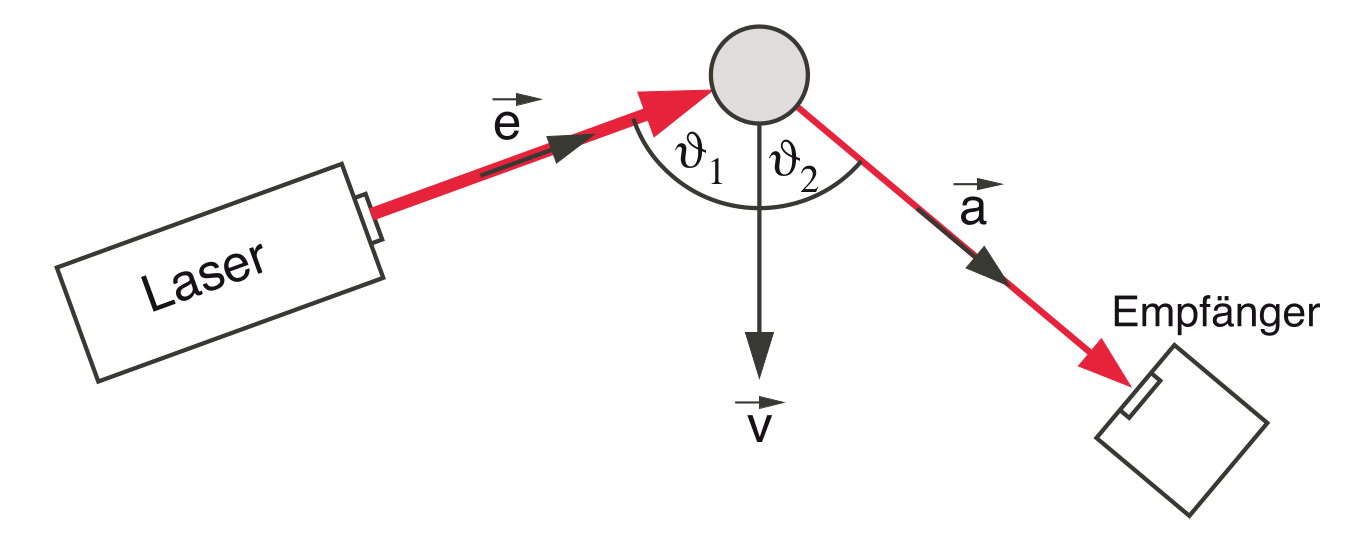
\includegraphics[width=0.67\textwidth]{images/doppler-effekt.png}
    \caption{%
        Dopplereffekt   mit  station\"arem   Sender,   bewegtem  Streuer   und
        station\"arem Detektor. \quelleVA
    }
    \label{fig:dopplereffekt}
\end{figure}

Da  bei  technischen  Geschwindigkeiten das  Verh\"altnis  $\frac{v}{c}$  sehr
klein   ist,  ergeben   sich  unter   solchen  Umst\"anden   lediglich  minime
Unterschide  in   den  Frequenzen  $f_4$,  $f_1$   und  $f_2$. Eine  pr\"azise
Messung  der  Frequenzunterschiede  ist  somit enorm  schwierig,  weshalb  man
sich  eines Zwei-Stral-Verfahrens  bedient. Da die  beiden Teilstrahlen  dabei
in  unterschiedlichen  Winkeln  $\vartheta_1$  (vgl. Formel  \ref{eq:doppler})
auf   das   streuende   Teilchen  treffen,   erfahren   sie   unterschiedliche
Doppler-Verschiebungen ihrer Frequenzen.

\"Uberlagert man  nun die beiden  Teilstrahlen in einem Detektor,  ergibt sich
eine  Schwebung, deren  Frequenz bedeutend  tiefer  als $f_0$  ist, und  somit
verh\"altnism\"assig gut detektiert werden kann.

Eine     h\"aufig     verwendete     Konfiguration    ist     in     Abbildung
\ref{fig:zweistrahl-anordnung} zu sehen.

\begin{figure}[h!t]
    \centering
    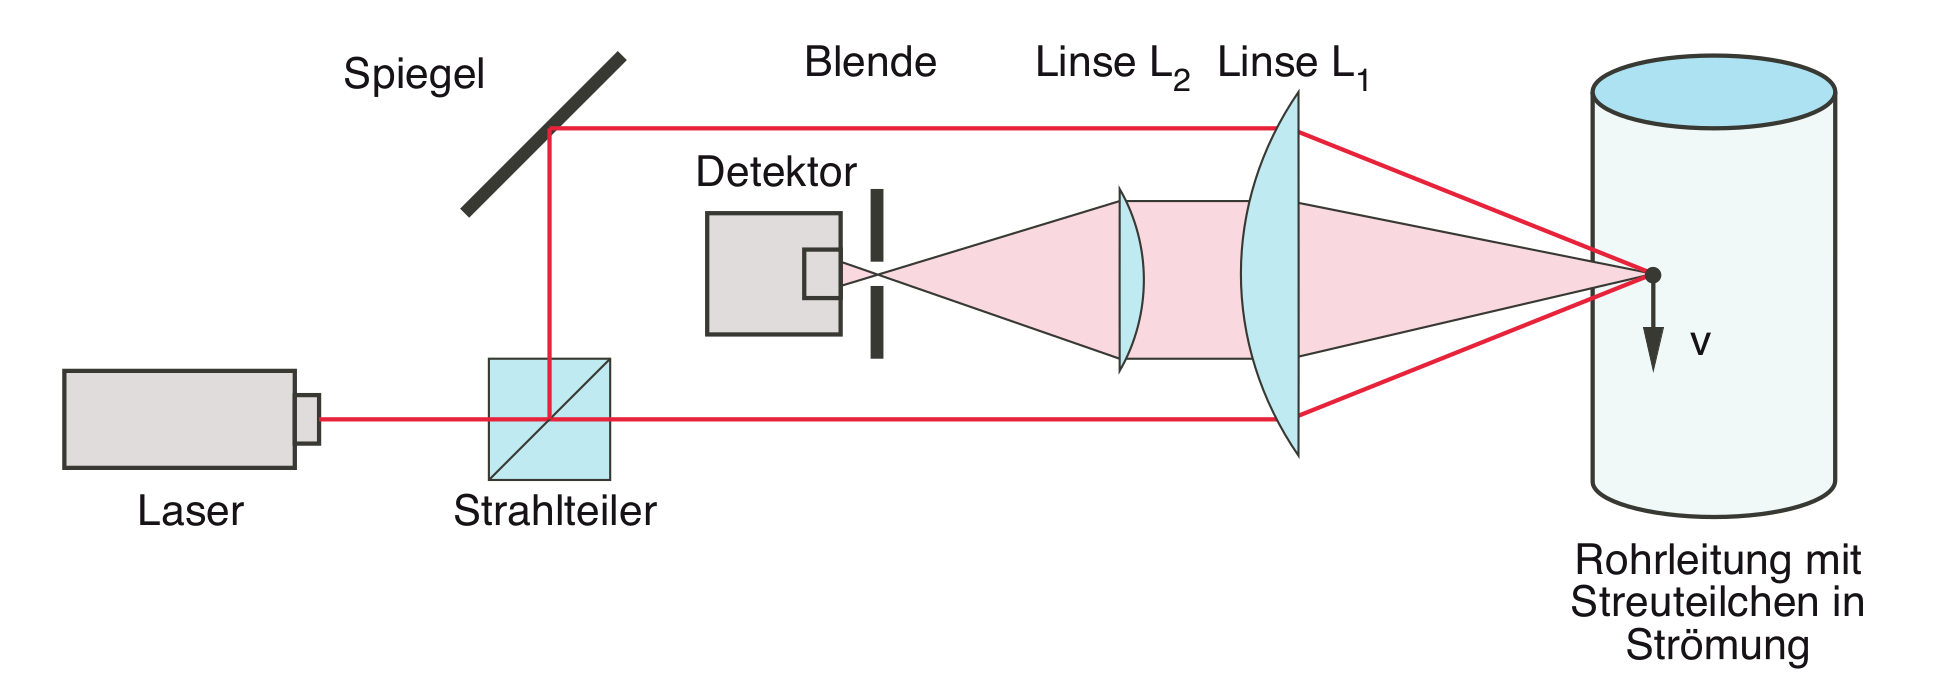
\includegraphics[width=0.67\textwidth]{images/zweistrahl-anordnung.png}
    \caption{%
        Zwei-Srahl-Anordnung. \quelleVA
    }
    \label{fig:zweistrahl-anordnung}
\end{figure}

Ein Strahlteiler teilt  den Laserstrahl auf zwei Strahlen auf  und ein Spiegel
sorgt daf\"ur, dass zwei parallele  Strahlen entstehen, die anschliessen durch
eine Linse $L_1$ mit Brennweite $f_1$ wieder zusammengef\"uhrt werden. Fliesst
ein Streuteilchen durch diesen Schnittpunkt, ergeben sich f\"ur die beiden Teilstrahlen
zwei unterschiedliche Frequenzen aufgrund des Dopplereffekts:

\begin{align}
    \label{eq:splitFreqs1}
        f_1 &= f_0 \cdot
            \left(
                1 + \frac{v}{c} \cdot \cos\left( \SI{90}{\degree} + \frac{\varphi}{2} \right)
            \right)
            =
            f_0 \cdot
            \left(
                1 - \frac{v}{c} \cdot \sin\left(\frac{\varphi}{2}\right)
            \right)
            \\
        \label{eq:splitFreqs2}
        f_2 &= f_0 \cdot
            \left(
                1 + \frac{v}{c} \cdot \cos\left( \SI{90}{\degree} - \frac{\varphi}{2} \right)
            \right)
            =
            f_0 \cdot
            \left(
                1 + \frac{v}{c} \cdot \sin\left(\frac{\varphi}{2}\right)
            \right)
            \\
        \label{eq:splitFreqsDelta}
        \Delta f &= f_2 - f_1 = f_0 \cdot \frac{2 \cdot v}{c} \cdot \sin\left( \frac{\varphi}{2}\right)
\end{align}

Die beiden  Wellenz\"uge werden  anschliessend in einem  einzelnen Empf\"anger
zusammengef\"uhrt. Die durch diese \"Uberlagerung erzeugte Schwebung errechnet
sich  nach  einigen  trigonometrischen  Umformungen zu  (beachte,  dass  beide
Signale die gleiche Amplitude haben, was die Sache etwas vereinfacht):

\begin{equation}
    \label{eq:schwebung}
    S(t) = A \cdot \cos(\omega_1 \cdot t) + A \cdot \cos(\omega_2 \cdot t)
         = 2 A \cdot
             \cos\left(
                 \frac{\omega_1 + \omega_2}{2} \cdot t
             \right)
             \cdot
             \cos\left(
                 \frac{\omega_1 - \omega_2}{2} \cdot t
             \right)
\end{equation}

% ---------------------------------------------------------------------------- %
\clearpage
\subsection{Grundlagen aus der Fluid-Dynamik}
\label{subsec:fluiddynamik}
% ---------------------------------------------------------------------------- %

\subsubsection{Vorbereitung auf Messaufgaben}

3.1 -- Zusammenhang zwischen maximaler und durchschnittlicher Str\"omungsgeschwindigkeit im laminaren Fall

\textbf{fix: avg over flaeche}
\begin{equation}
    \label{eq:laminar:v_max:v_avg}
    \frac{v(r)}{v_{max}} = \frac{1}{v_{max} \cdot R} \cdot \int_0^R\!v(r) \, \mathrm{d}r
    = \frac{1}{R} \cdot \int_0^R \! 1 - \frac{r^2}{R^2} \, \mathrm{d}r
    = \frac{1}{2}
\end{equation}

3.2 -- Zusammenhang zwischen maximaler und durchschnittlicher Str\"omungsgeschwindigkeit im turbulenten Fall:

\begin{align}
    \label{eq:turbulent:v_max:v_avg}
    v(r) &= v_{max} \cdot \left( 1 - \frac{r}{R} \right) ^ \frac{1}{k}
    \\
    v_m &= \frac{1}{\pi \cdot R^2} \cdot \int_0^R \! v(r) \cdot 2 \cdot \pi \cdot r \, \mathrm{d}r
    \\
    \frac{v_m}{v_{max}} &= \frac{2}{R^2} \cdot \int_0^R \! \left(1 - \frac{r}{R} \right) ^ \frac{1}{k} \cdot r \, \mathrm{d}r = \frac{2 \cdot k^2}{(k + 1) \cdot (2k + 1)}
\end{align}

3.3 -- Vergleich von laminarem und turbulentem Str\"omungsprofil

%\begin{figure}[h!t]
%    \centering
%    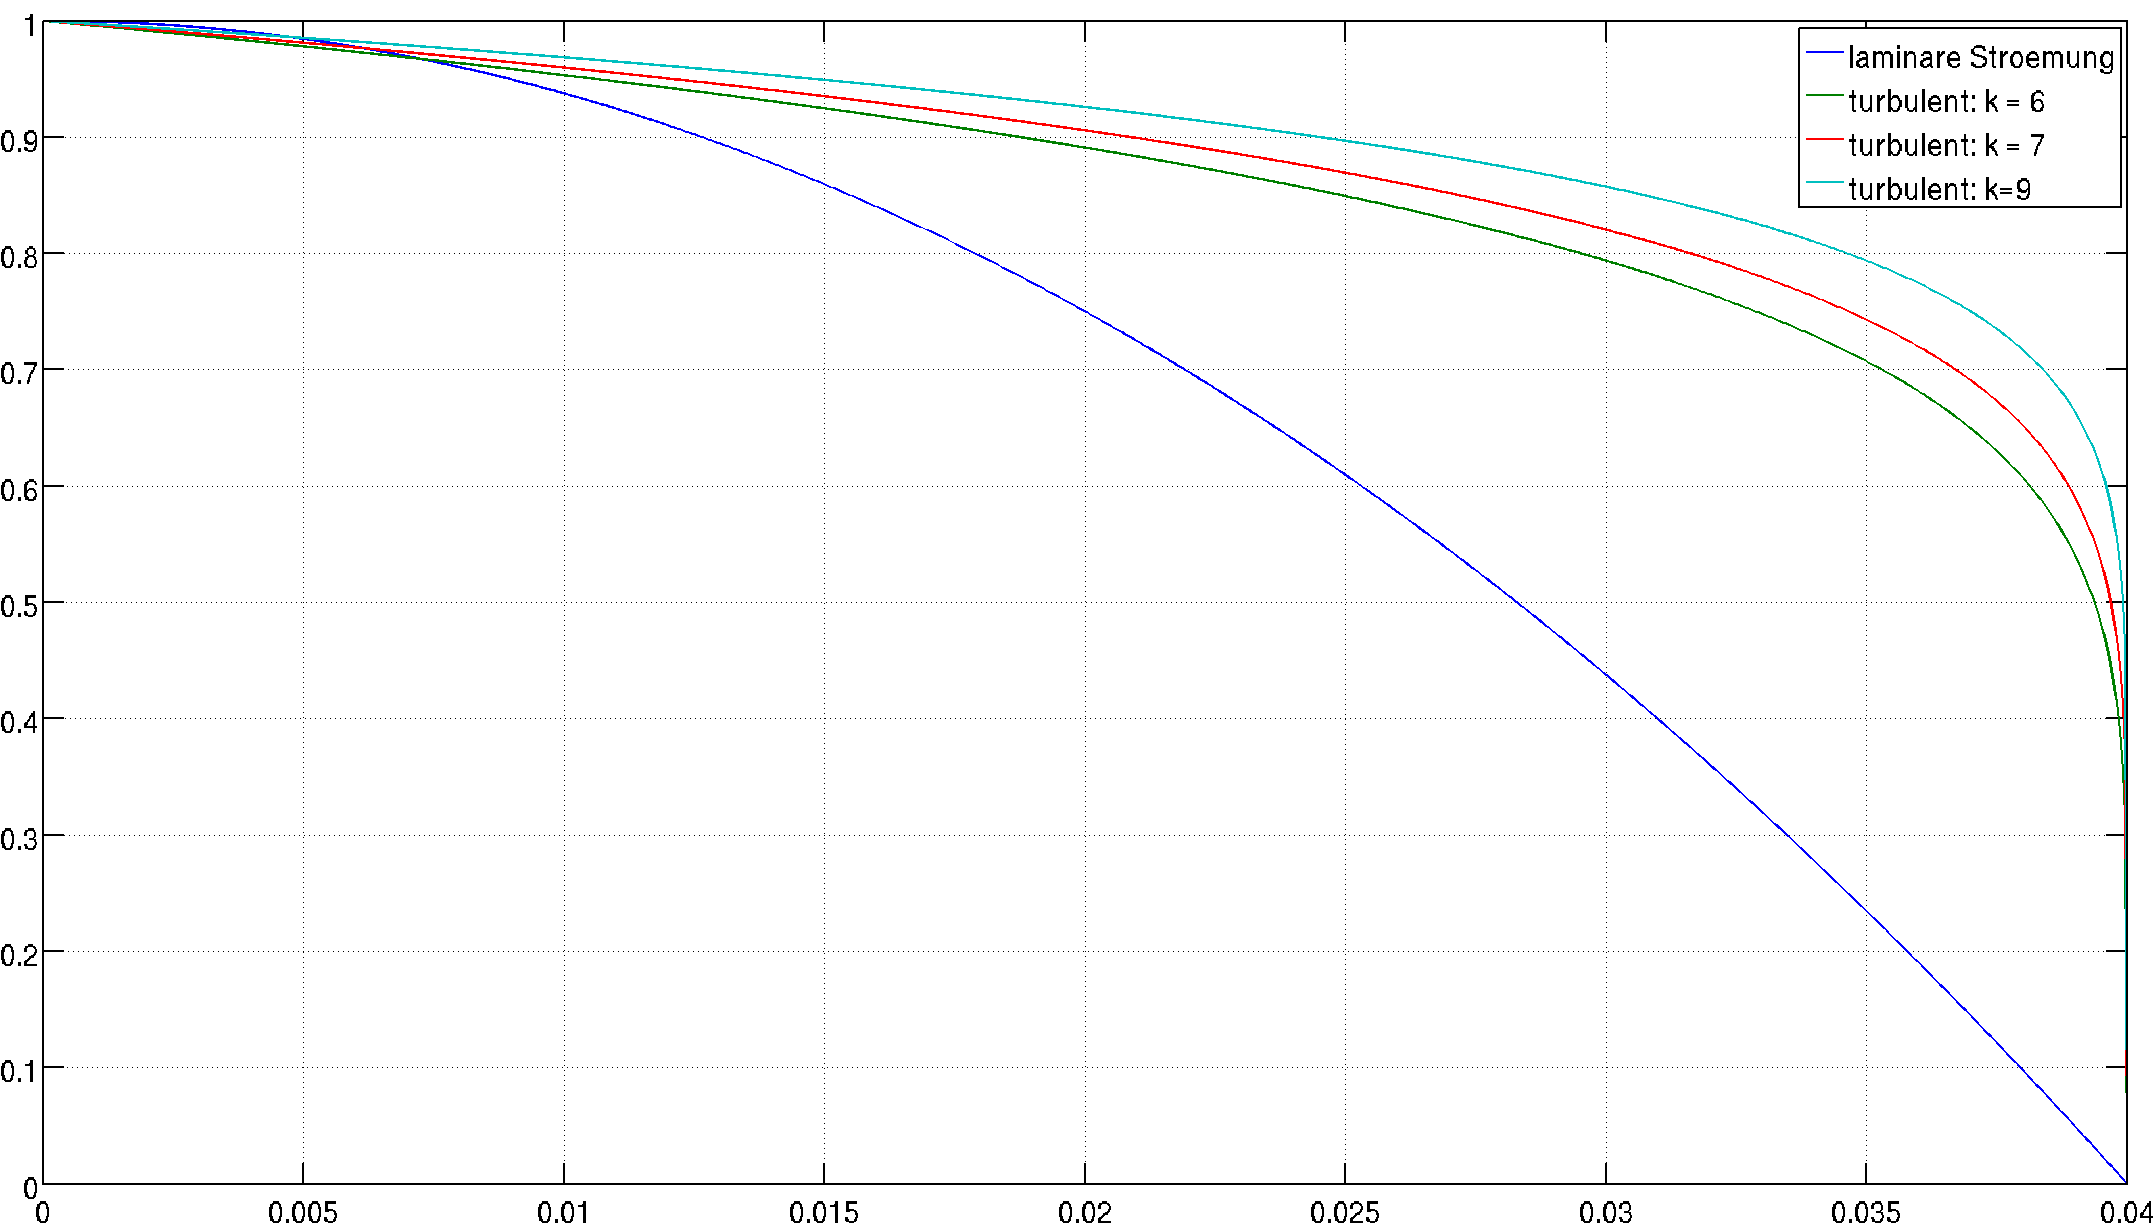
\includegraphics[width=\textwidth]{images/laminar-vs-turbulent.png}
%    \caption{%
%        Laminares vs. turbulente Str\"omungsprofile
%    }
%    \label{fig:dopplereffekt}
%\end{figure}

\begin{figure}[h!t]
    \centering
    \resizebox{.9\textwidth}{!}{%% Creator: Matplotlib, PGF backend
%%
%% To include the figure in your LaTeX document, write
%%   \input{<filename>.pgf}
%%
%% Make sure the required packages are loaded in your preamble
%%   \usepackage{pgf}
%%
%% Figures using additional raster images can only be included by \input if
%% they are in the same directory as the main LaTeX file. For loading figures
%% from other directories you can use the `import` package
%%   \usepackage{import}
%% and then include the figures with
%%   \import{<path to file>}{<filename>.pgf}
%%
%% Matplotlib used the following preamble
%%   \usepackage{fontspec}
%%   \setmainfont{Bitstream Vera Serif}
%%   \setsansfont{Bitstream Vera Sans}
%%   \setmonofont{Bitstream Vera Sans Mono}
%%
\begingroup%
\makeatletter%
\begin{pgfpicture}%
\pgfpathrectangle{\pgfpointorigin}{\pgfqpoint{8.000000in}{6.000000in}}%
\pgfusepath{use as bounding box, clip}%
\begin{pgfscope}%
\pgfsetbuttcap%
\pgfsetmiterjoin%
\definecolor{currentfill}{rgb}{1.000000,1.000000,1.000000}%
\pgfsetfillcolor{currentfill}%
\pgfsetlinewidth{0.000000pt}%
\definecolor{currentstroke}{rgb}{1.000000,1.000000,1.000000}%
\pgfsetstrokecolor{currentstroke}%
\pgfsetdash{}{0pt}%
\pgfpathmoveto{\pgfqpoint{0.000000in}{0.000000in}}%
\pgfpathlineto{\pgfqpoint{8.000000in}{0.000000in}}%
\pgfpathlineto{\pgfqpoint{8.000000in}{6.000000in}}%
\pgfpathlineto{\pgfqpoint{0.000000in}{6.000000in}}%
\pgfpathclose%
\pgfusepath{fill}%
\end{pgfscope}%
\begin{pgfscope}%
\pgfsetbuttcap%
\pgfsetmiterjoin%
\definecolor{currentfill}{rgb}{1.000000,1.000000,1.000000}%
\pgfsetfillcolor{currentfill}%
\pgfsetlinewidth{0.000000pt}%
\definecolor{currentstroke}{rgb}{0.000000,0.000000,0.000000}%
\pgfsetstrokecolor{currentstroke}%
\pgfsetstrokeopacity{0.000000}%
\pgfsetdash{}{0pt}%
\pgfpathmoveto{\pgfqpoint{1.000000in}{0.600000in}}%
\pgfpathlineto{\pgfqpoint{7.200000in}{0.600000in}}%
\pgfpathlineto{\pgfqpoint{7.200000in}{5.400000in}}%
\pgfpathlineto{\pgfqpoint{1.000000in}{5.400000in}}%
\pgfpathclose%
\pgfusepath{fill}%
\end{pgfscope}%
\begin{pgfscope}%
\pgfpathrectangle{\pgfqpoint{1.000000in}{0.600000in}}{\pgfqpoint{6.200000in}{4.800000in}} %
\pgfusepath{clip}%
\pgfsetrectcap%
\pgfsetroundjoin%
\pgfsetlinewidth{1.003750pt}%
\definecolor{currentstroke}{rgb}{0.000000,0.000000,1.000000}%
\pgfsetstrokecolor{currentstroke}%
\pgfsetdash{}{0pt}%
\pgfpathmoveto{\pgfqpoint{1.000000in}{5.400000in}}%
\pgfpathlineto{\pgfqpoint{1.091268in}{5.398918in}}%
\pgfpathlineto{\pgfqpoint{1.182535in}{5.395671in}}%
\pgfpathlineto{\pgfqpoint{1.273803in}{5.390261in}}%
\pgfpathlineto{\pgfqpoint{1.365071in}{5.382685in}}%
\pgfpathlineto{\pgfqpoint{1.456339in}{5.372946in}}%
\pgfpathlineto{\pgfqpoint{1.547606in}{5.361042in}}%
\pgfpathlineto{\pgfqpoint{1.638874in}{5.346974in}}%
\pgfpathlineto{\pgfqpoint{1.730142in}{5.330742in}}%
\pgfpathlineto{\pgfqpoint{1.821410in}{5.312345in}}%
\pgfpathlineto{\pgfqpoint{1.912677in}{5.291784in}}%
\pgfpathlineto{\pgfqpoint{2.003945in}{5.269058in}}%
\pgfpathlineto{\pgfqpoint{2.095213in}{5.244168in}}%
\pgfpathlineto{\pgfqpoint{2.192565in}{5.215234in}}%
\pgfpathlineto{\pgfqpoint{2.289917in}{5.183837in}}%
\pgfpathlineto{\pgfqpoint{2.387270in}{5.149977in}}%
\pgfpathlineto{\pgfqpoint{2.484622in}{5.113655in}}%
\pgfpathlineto{\pgfqpoint{2.581974in}{5.074870in}}%
\pgfpathlineto{\pgfqpoint{2.679326in}{5.033623in}}%
\pgfpathlineto{\pgfqpoint{2.776679in}{4.989913in}}%
\pgfpathlineto{\pgfqpoint{2.874031in}{4.943741in}}%
\pgfpathlineto{\pgfqpoint{2.971383in}{4.895106in}}%
\pgfpathlineto{\pgfqpoint{3.068735in}{4.844009in}}%
\pgfpathlineto{\pgfqpoint{3.166088in}{4.790449in}}%
\pgfpathlineto{\pgfqpoint{3.263440in}{4.734426in}}%
\pgfpathlineto{\pgfqpoint{3.360792in}{4.675941in}}%
\pgfpathlineto{\pgfqpoint{3.458144in}{4.614994in}}%
\pgfpathlineto{\pgfqpoint{3.561581in}{4.547539in}}%
\pgfpathlineto{\pgfqpoint{3.665018in}{4.477304in}}%
\pgfpathlineto{\pgfqpoint{3.768455in}{4.404290in}}%
\pgfpathlineto{\pgfqpoint{3.871891in}{4.328495in}}%
\pgfpathlineto{\pgfqpoint{3.975328in}{4.249920in}}%
\pgfpathlineto{\pgfqpoint{4.078765in}{4.168566in}}%
\pgfpathlineto{\pgfqpoint{4.182202in}{4.084431in}}%
\pgfpathlineto{\pgfqpoint{4.285639in}{3.997516in}}%
\pgfpathlineto{\pgfqpoint{4.389075in}{3.907822in}}%
\pgfpathlineto{\pgfqpoint{4.498597in}{3.809821in}}%
\pgfpathlineto{\pgfqpoint{4.608118in}{3.708704in}}%
\pgfpathlineto{\pgfqpoint{4.717639in}{3.604470in}}%
\pgfpathlineto{\pgfqpoint{4.827160in}{3.497119in}}%
\pgfpathlineto{\pgfqpoint{4.936682in}{3.386652in}}%
\pgfpathlineto{\pgfqpoint{5.046203in}{3.273068in}}%
\pgfpathlineto{\pgfqpoint{5.155724in}{3.156368in}}%
\pgfpathlineto{\pgfqpoint{5.265246in}{3.036551in}}%
\pgfpathlineto{\pgfqpoint{5.380851in}{2.906696in}}%
\pgfpathlineto{\pgfqpoint{5.496457in}{2.773369in}}%
\pgfpathlineto{\pgfqpoint{5.612063in}{2.636569in}}%
\pgfpathlineto{\pgfqpoint{5.727669in}{2.496296in}}%
\pgfpathlineto{\pgfqpoint{5.843275in}{2.352551in}}%
\pgfpathlineto{\pgfqpoint{5.958880in}{2.205334in}}%
\pgfpathlineto{\pgfqpoint{6.074486in}{2.054644in}}%
\pgfpathlineto{\pgfqpoint{6.196177in}{1.892271in}}%
\pgfpathlineto{\pgfqpoint{6.317867in}{1.726051in}}%
\pgfpathlineto{\pgfqpoint{6.439557in}{1.555983in}}%
\pgfpathlineto{\pgfqpoint{6.561248in}{1.382067in}}%
\pgfpathlineto{\pgfqpoint{6.682938in}{1.204304in}}%
\pgfpathlineto{\pgfqpoint{6.804628in}{1.022693in}}%
\pgfpathlineto{\pgfqpoint{6.926318in}{0.837234in}}%
\pgfpathlineto{\pgfqpoint{7.054093in}{0.638361in}}%
\pgfpathlineto{\pgfqpoint{7.078431in}{0.600000in}}%
\pgfpathlineto{\pgfqpoint{7.078431in}{0.600000in}}%
\pgfusepath{stroke}%
\end{pgfscope}%
\begin{pgfscope}%
\pgfpathrectangle{\pgfqpoint{1.000000in}{0.600000in}}{\pgfqpoint{6.200000in}{4.800000in}} %
\pgfusepath{clip}%
\pgfsetrectcap%
\pgfsetroundjoin%
\pgfsetlinewidth{1.003750pt}%
\definecolor{currentstroke}{rgb}{0.000000,0.500000,0.000000}%
\pgfsetstrokecolor{currentstroke}%
\pgfsetdash{}{0pt}%
\pgfpathmoveto{\pgfqpoint{1.000000in}{5.400000in}}%
\pgfpathlineto{\pgfqpoint{1.346817in}{5.353230in}}%
\pgfpathlineto{\pgfqpoint{1.675381in}{5.306692in}}%
\pgfpathlineto{\pgfqpoint{1.985692in}{5.260522in}}%
\pgfpathlineto{\pgfqpoint{2.277748in}{5.214874in}}%
\pgfpathlineto{\pgfqpoint{2.557636in}{5.168901in}}%
\pgfpathlineto{\pgfqpoint{2.819270in}{5.123730in}}%
\pgfpathlineto{\pgfqpoint{3.068735in}{5.078452in}}%
\pgfpathlineto{\pgfqpoint{3.306032in}{5.033148in}}%
\pgfpathlineto{\pgfqpoint{3.531159in}{4.987917in}}%
\pgfpathlineto{\pgfqpoint{3.744117in}{4.942873in}}%
\pgfpathlineto{\pgfqpoint{3.944906in}{4.898150in}}%
\pgfpathlineto{\pgfqpoint{4.133526in}{4.853906in}}%
\pgfpathlineto{\pgfqpoint{4.316061in}{4.808781in}}%
\pgfpathlineto{\pgfqpoint{4.486428in}{4.764363in}}%
\pgfpathlineto{\pgfqpoint{4.644625in}{4.720883in}}%
\pgfpathlineto{\pgfqpoint{4.796738in}{4.676795in}}%
\pgfpathlineto{\pgfqpoint{4.942766in}{4.632102in}}%
\pgfpathlineto{\pgfqpoint{5.076626in}{4.588837in}}%
\pgfpathlineto{\pgfqpoint{5.204400in}{4.545228in}}%
\pgfpathlineto{\pgfqpoint{5.326091in}{4.501327in}}%
\pgfpathlineto{\pgfqpoint{5.441697in}{4.457202in}}%
\pgfpathlineto{\pgfqpoint{5.551218in}{4.412934in}}%
\pgfpathlineto{\pgfqpoint{5.654655in}{4.368625in}}%
\pgfpathlineto{\pgfqpoint{5.752007in}{4.324401in}}%
\pgfpathlineto{\pgfqpoint{5.843275in}{4.280411in}}%
\pgfpathlineto{\pgfqpoint{5.928458in}{4.236838in}}%
\pgfpathlineto{\pgfqpoint{6.007557in}{4.193898in}}%
\pgfpathlineto{\pgfqpoint{6.080571in}{4.151847in}}%
\pgfpathlineto{\pgfqpoint{6.153585in}{4.107149in}}%
\pgfpathlineto{\pgfqpoint{6.220515in}{4.063513in}}%
\pgfpathlineto{\pgfqpoint{6.281360in}{4.021308in}}%
\pgfpathlineto{\pgfqpoint{6.342205in}{3.976327in}}%
\pgfpathlineto{\pgfqpoint{6.396966in}{3.933113in}}%
\pgfpathlineto{\pgfqpoint{6.451726in}{3.886900in}}%
\pgfpathlineto{\pgfqpoint{6.500402in}{3.842905in}}%
\pgfpathlineto{\pgfqpoint{6.549078in}{3.795706in}}%
\pgfpathlineto{\pgfqpoint{6.591670in}{3.751340in}}%
\pgfpathlineto{\pgfqpoint{6.634262in}{3.703612in}}%
\pgfpathlineto{\pgfqpoint{6.670769in}{3.659563in}}%
\pgfpathlineto{\pgfqpoint{6.707276in}{3.612095in}}%
\pgfpathlineto{\pgfqpoint{6.743783in}{3.560562in}}%
\pgfpathlineto{\pgfqpoint{6.774206in}{3.513905in}}%
\pgfpathlineto{\pgfqpoint{6.804628in}{3.463183in}}%
\pgfpathlineto{\pgfqpoint{6.835051in}{3.407525in}}%
\pgfpathlineto{\pgfqpoint{6.859389in}{3.358655in}}%
\pgfpathlineto{\pgfqpoint{6.883727in}{3.305029in}}%
\pgfpathlineto{\pgfqpoint{6.908065in}{3.245493in}}%
\pgfpathlineto{\pgfqpoint{6.926318in}{3.195994in}}%
\pgfpathlineto{\pgfqpoint{6.944572in}{3.141270in}}%
\pgfpathlineto{\pgfqpoint{6.962826in}{3.079929in}}%
\pgfpathlineto{\pgfqpoint{6.981079in}{3.009907in}}%
\pgfpathlineto{\pgfqpoint{6.999333in}{2.927935in}}%
\pgfpathlineto{\pgfqpoint{7.011502in}{2.864014in}}%
\pgfpathlineto{\pgfqpoint{7.023671in}{2.789546in}}%
\pgfpathlineto{\pgfqpoint{7.035840in}{2.699729in}}%
\pgfpathlineto{\pgfqpoint{7.048009in}{2.585220in}}%
\pgfpathlineto{\pgfqpoint{7.054093in}{2.512745in}}%
\pgfpathlineto{\pgfqpoint{7.060178in}{2.423198in}}%
\pgfpathlineto{\pgfqpoint{7.066262in}{2.304062in}}%
\pgfpathlineto{\pgfqpoint{7.072347in}{2.118146in}}%
\pgfpathlineto{\pgfqpoint{7.078431in}{0.600000in}}%
\pgfpathlineto{\pgfqpoint{7.078431in}{0.600000in}}%
\pgfusepath{stroke}%
\end{pgfscope}%
\begin{pgfscope}%
\pgfpathrectangle{\pgfqpoint{1.000000in}{0.600000in}}{\pgfqpoint{6.200000in}{4.800000in}} %
\pgfusepath{clip}%
\pgfsetrectcap%
\pgfsetroundjoin%
\pgfsetlinewidth{1.003750pt}%
\definecolor{currentstroke}{rgb}{1.000000,0.000000,0.000000}%
\pgfsetstrokecolor{currentstroke}%
\pgfsetdash{}{0pt}%
\pgfpathmoveto{\pgfqpoint{1.000000in}{5.400000in}}%
\pgfpathlineto{\pgfqpoint{1.365071in}{5.357715in}}%
\pgfpathlineto{\pgfqpoint{1.711888in}{5.315341in}}%
\pgfpathlineto{\pgfqpoint{2.040452in}{5.272974in}}%
\pgfpathlineto{\pgfqpoint{2.350763in}{5.230727in}}%
\pgfpathlineto{\pgfqpoint{2.642819in}{5.188735in}}%
\pgfpathlineto{\pgfqpoint{2.916623in}{5.147156in}}%
\pgfpathlineto{\pgfqpoint{3.178257in}{5.105174in}}%
\pgfpathlineto{\pgfqpoint{3.421637in}{5.063895in}}%
\pgfpathlineto{\pgfqpoint{3.652849in}{5.022437in}}%
\pgfpathlineto{\pgfqpoint{3.871891in}{4.980886in}}%
\pgfpathlineto{\pgfqpoint{4.078765in}{4.939346in}}%
\pgfpathlineto{\pgfqpoint{4.273470in}{4.897942in}}%
\pgfpathlineto{\pgfqpoint{4.456005in}{4.856825in}}%
\pgfpathlineto{\pgfqpoint{4.626371in}{4.816172in}}%
\pgfpathlineto{\pgfqpoint{4.784569in}{4.776194in}}%
\pgfpathlineto{\pgfqpoint{4.936682in}{4.735459in}}%
\pgfpathlineto{\pgfqpoint{5.076626in}{4.695730in}}%
\pgfpathlineto{\pgfqpoint{5.210485in}{4.655434in}}%
\pgfpathlineto{\pgfqpoint{5.338260in}{4.614591in}}%
\pgfpathlineto{\pgfqpoint{5.453866in}{4.575359in}}%
\pgfpathlineto{\pgfqpoint{5.563387in}{4.535918in}}%
\pgfpathlineto{\pgfqpoint{5.666824in}{4.496357in}}%
\pgfpathlineto{\pgfqpoint{5.764176in}{4.456784in}}%
\pgfpathlineto{\pgfqpoint{5.855444in}{4.417332in}}%
\pgfpathlineto{\pgfqpoint{5.940627in}{4.378163in}}%
\pgfpathlineto{\pgfqpoint{6.019726in}{4.339473in}}%
\pgfpathlineto{\pgfqpoint{6.098824in}{4.298220in}}%
\pgfpathlineto{\pgfqpoint{6.171839in}{4.257523in}}%
\pgfpathlineto{\pgfqpoint{6.238768in}{4.217670in}}%
\pgfpathlineto{\pgfqpoint{6.299613in}{4.179001in}}%
\pgfpathlineto{\pgfqpoint{6.360458in}{4.137651in}}%
\pgfpathlineto{\pgfqpoint{6.415219in}{4.097783in}}%
\pgfpathlineto{\pgfqpoint{6.469980in}{4.054985in}}%
\pgfpathlineto{\pgfqpoint{6.518656in}{4.014075in}}%
\pgfpathlineto{\pgfqpoint{6.567332in}{3.969992in}}%
\pgfpathlineto{\pgfqpoint{6.609924in}{3.928362in}}%
\pgfpathlineto{\pgfqpoint{6.652515in}{3.883351in}}%
\pgfpathlineto{\pgfqpoint{6.689022in}{3.841586in}}%
\pgfpathlineto{\pgfqpoint{6.725529in}{3.796319in}}%
\pgfpathlineto{\pgfqpoint{6.755952in}{3.755419in}}%
\pgfpathlineto{\pgfqpoint{6.786375in}{3.711066in}}%
\pgfpathlineto{\pgfqpoint{6.816797in}{3.662559in}}%
\pgfpathlineto{\pgfqpoint{6.841135in}{3.620138in}}%
\pgfpathlineto{\pgfqpoint{6.865473in}{3.573809in}}%
\pgfpathlineto{\pgfqpoint{6.889811in}{3.522695in}}%
\pgfpathlineto{\pgfqpoint{6.914149in}{3.465579in}}%
\pgfpathlineto{\pgfqpoint{6.932403in}{3.417766in}}%
\pgfpathlineto{\pgfqpoint{6.950657in}{3.364524in}}%
\pgfpathlineto{\pgfqpoint{6.968910in}{3.304310in}}%
\pgfpathlineto{\pgfqpoint{6.987164in}{3.234783in}}%
\pgfpathlineto{\pgfqpoint{6.999333in}{3.181467in}}%
\pgfpathlineto{\pgfqpoint{7.011502in}{3.120590in}}%
\pgfpathlineto{\pgfqpoint{7.023671in}{3.049358in}}%
\pgfpathlineto{\pgfqpoint{7.035840in}{2.962981in}}%
\pgfpathlineto{\pgfqpoint{7.048009in}{2.852085in}}%
\pgfpathlineto{\pgfqpoint{7.054093in}{2.781426in}}%
\pgfpathlineto{\pgfqpoint{7.060178in}{2.693592in}}%
\pgfpathlineto{\pgfqpoint{7.066262in}{2.575769in}}%
\pgfpathlineto{\pgfqpoint{7.072347in}{2.389501in}}%
\pgfpathlineto{\pgfqpoint{7.078431in}{0.600000in}}%
\pgfpathlineto{\pgfqpoint{7.078431in}{0.600000in}}%
\pgfusepath{stroke}%
\end{pgfscope}%
\begin{pgfscope}%
\pgfpathrectangle{\pgfqpoint{1.000000in}{0.600000in}}{\pgfqpoint{6.200000in}{4.800000in}} %
\pgfusepath{clip}%
\pgfsetrectcap%
\pgfsetroundjoin%
\pgfsetlinewidth{1.003750pt}%
\definecolor{currentstroke}{rgb}{0.000000,0.750000,0.750000}%
\pgfsetstrokecolor{currentstroke}%
\pgfsetdash{}{0pt}%
\pgfpathmoveto{\pgfqpoint{1.000000in}{5.400000in}}%
\pgfpathlineto{\pgfqpoint{1.407663in}{5.363117in}}%
\pgfpathlineto{\pgfqpoint{1.790987in}{5.326220in}}%
\pgfpathlineto{\pgfqpoint{2.149974in}{5.289442in}}%
\pgfpathlineto{\pgfqpoint{2.484622in}{5.252947in}}%
\pgfpathlineto{\pgfqpoint{2.794932in}{5.216928in}}%
\pgfpathlineto{\pgfqpoint{3.086989in}{5.180844in}}%
\pgfpathlineto{\pgfqpoint{3.360792in}{5.144816in}}%
\pgfpathlineto{\pgfqpoint{3.616342in}{5.108995in}}%
\pgfpathlineto{\pgfqpoint{3.853638in}{5.073562in}}%
\pgfpathlineto{\pgfqpoint{4.078765in}{5.037735in}}%
\pgfpathlineto{\pgfqpoint{4.291723in}{5.001573in}}%
\pgfpathlineto{\pgfqpoint{4.486428in}{4.966292in}}%
\pgfpathlineto{\pgfqpoint{4.668963in}{4.931008in}}%
\pgfpathlineto{\pgfqpoint{4.839330in}{4.895863in}}%
\pgfpathlineto{\pgfqpoint{4.997527in}{4.861030in}}%
\pgfpathlineto{\pgfqpoint{5.149640in}{4.825243in}}%
\pgfpathlineto{\pgfqpoint{5.289584in}{4.790029in}}%
\pgfpathlineto{\pgfqpoint{5.417359in}{4.755669in}}%
\pgfpathlineto{\pgfqpoint{5.539049in}{4.720686in}}%
\pgfpathlineto{\pgfqpoint{5.654655in}{4.685097in}}%
\pgfpathlineto{\pgfqpoint{5.758091in}{4.651005in}}%
\pgfpathlineto{\pgfqpoint{5.855444in}{4.616677in}}%
\pgfpathlineto{\pgfqpoint{5.946711in}{4.582211in}}%
\pgfpathlineto{\pgfqpoint{6.031895in}{4.547737in}}%
\pgfpathlineto{\pgfqpoint{6.110993in}{4.513415in}}%
\pgfpathlineto{\pgfqpoint{6.184008in}{4.479442in}}%
\pgfpathlineto{\pgfqpoint{6.250937in}{4.446060in}}%
\pgfpathlineto{\pgfqpoint{6.317867in}{4.410186in}}%
\pgfpathlineto{\pgfqpoint{6.378712in}{4.375049in}}%
\pgfpathlineto{\pgfqpoint{6.433473in}{4.341021in}}%
\pgfpathlineto{\pgfqpoint{6.488233in}{4.304321in}}%
\pgfpathlineto{\pgfqpoint{6.536909in}{4.269062in}}%
\pgfpathlineto{\pgfqpoint{6.585586in}{4.230865in}}%
\pgfpathlineto{\pgfqpoint{6.628177in}{4.194584in}}%
\pgfpathlineto{\pgfqpoint{6.670769in}{4.155113in}}%
\pgfpathlineto{\pgfqpoint{6.707276in}{4.118246in}}%
\pgfpathlineto{\pgfqpoint{6.743783in}{4.078002in}}%
\pgfpathlineto{\pgfqpoint{6.774206in}{4.041364in}}%
\pgfpathlineto{\pgfqpoint{6.804628in}{4.001312in}}%
\pgfpathlineto{\pgfqpoint{6.835051in}{3.957089in}}%
\pgfpathlineto{\pgfqpoint{6.859389in}{3.918018in}}%
\pgfpathlineto{\pgfqpoint{6.883727in}{3.874878in}}%
\pgfpathlineto{\pgfqpoint{6.908065in}{3.826647in}}%
\pgfpathlineto{\pgfqpoint{6.926318in}{3.786272in}}%
\pgfpathlineto{\pgfqpoint{6.944572in}{3.741335in}}%
\pgfpathlineto{\pgfqpoint{6.962826in}{3.690579in}}%
\pgfpathlineto{\pgfqpoint{6.981079in}{3.632126in}}%
\pgfpathlineto{\pgfqpoint{6.993248in}{3.587471in}}%
\pgfpathlineto{\pgfqpoint{7.005417in}{3.536738in}}%
\pgfpathlineto{\pgfqpoint{7.017586in}{3.477844in}}%
\pgfpathlineto{\pgfqpoint{7.029755in}{3.407369in}}%
\pgfpathlineto{\pgfqpoint{7.041924in}{3.319051in}}%
\pgfpathlineto{\pgfqpoint{7.048009in}{3.264523in}}%
\pgfpathlineto{\pgfqpoint{7.054093in}{3.199272in}}%
\pgfpathlineto{\pgfqpoint{7.060178in}{3.117501in}}%
\pgfpathlineto{\pgfqpoint{7.066262in}{3.006600in}}%
\pgfpathlineto{\pgfqpoint{7.072347in}{2.828210in}}%
\pgfpathlineto{\pgfqpoint{7.078431in}{0.600000in}}%
\pgfpathlineto{\pgfqpoint{7.078431in}{0.600000in}}%
\pgfusepath{stroke}%
\end{pgfscope}%
\begin{pgfscope}%
\pgfsetrectcap%
\pgfsetmiterjoin%
\pgfsetlinewidth{1.003750pt}%
\definecolor{currentstroke}{rgb}{0.000000,0.000000,0.000000}%
\pgfsetstrokecolor{currentstroke}%
\pgfsetdash{}{0pt}%
\pgfpathmoveto{\pgfqpoint{7.200000in}{0.600000in}}%
\pgfpathlineto{\pgfqpoint{7.200000in}{5.400000in}}%
\pgfusepath{stroke}%
\end{pgfscope}%
\begin{pgfscope}%
\pgfsetrectcap%
\pgfsetmiterjoin%
\pgfsetlinewidth{1.003750pt}%
\definecolor{currentstroke}{rgb}{0.000000,0.000000,0.000000}%
\pgfsetstrokecolor{currentstroke}%
\pgfsetdash{}{0pt}%
\pgfpathmoveto{\pgfqpoint{1.000000in}{0.600000in}}%
\pgfpathlineto{\pgfqpoint{1.000000in}{5.400000in}}%
\pgfusepath{stroke}%
\end{pgfscope}%
\begin{pgfscope}%
\pgfsetrectcap%
\pgfsetmiterjoin%
\pgfsetlinewidth{1.003750pt}%
\definecolor{currentstroke}{rgb}{0.000000,0.000000,0.000000}%
\pgfsetstrokecolor{currentstroke}%
\pgfsetdash{}{0pt}%
\pgfpathmoveto{\pgfqpoint{1.000000in}{5.400000in}}%
\pgfpathlineto{\pgfqpoint{7.200000in}{5.400000in}}%
\pgfusepath{stroke}%
\end{pgfscope}%
\begin{pgfscope}%
\pgfsetrectcap%
\pgfsetmiterjoin%
\pgfsetlinewidth{1.003750pt}%
\definecolor{currentstroke}{rgb}{0.000000,0.000000,0.000000}%
\pgfsetstrokecolor{currentstroke}%
\pgfsetdash{}{0pt}%
\pgfpathmoveto{\pgfqpoint{1.000000in}{0.600000in}}%
\pgfpathlineto{\pgfqpoint{7.200000in}{0.600000in}}%
\pgfusepath{stroke}%
\end{pgfscope}%
\begin{pgfscope}%
\pgfsetbuttcap%
\pgfsetroundjoin%
\definecolor{currentfill}{rgb}{0.000000,0.000000,0.000000}%
\pgfsetfillcolor{currentfill}%
\pgfsetlinewidth{0.501875pt}%
\definecolor{currentstroke}{rgb}{0.000000,0.000000,0.000000}%
\pgfsetstrokecolor{currentstroke}%
\pgfsetdash{}{0pt}%
\pgfsys@defobject{currentmarker}{\pgfqpoint{0.000000in}{0.000000in}}{\pgfqpoint{0.000000in}{0.055556in}}{%
\pgfpathmoveto{\pgfqpoint{0.000000in}{0.000000in}}%
\pgfpathlineto{\pgfqpoint{0.000000in}{0.055556in}}%
\pgfusepath{stroke,fill}%
}%
\begin{pgfscope}%
\pgfsys@transformshift{1.000000in}{0.600000in}%
\pgfsys@useobject{currentmarker}{}%
\end{pgfscope}%
\end{pgfscope}%
\begin{pgfscope}%
\pgfsetbuttcap%
\pgfsetroundjoin%
\definecolor{currentfill}{rgb}{0.000000,0.000000,0.000000}%
\pgfsetfillcolor{currentfill}%
\pgfsetlinewidth{0.501875pt}%
\definecolor{currentstroke}{rgb}{0.000000,0.000000,0.000000}%
\pgfsetstrokecolor{currentstroke}%
\pgfsetdash{}{0pt}%
\pgfsys@defobject{currentmarker}{\pgfqpoint{0.000000in}{-0.055556in}}{\pgfqpoint{0.000000in}{0.000000in}}{%
\pgfpathmoveto{\pgfqpoint{0.000000in}{0.000000in}}%
\pgfpathlineto{\pgfqpoint{0.000000in}{-0.055556in}}%
\pgfusepath{stroke,fill}%
}%
\begin{pgfscope}%
\pgfsys@transformshift{1.000000in}{5.400000in}%
\pgfsys@useobject{currentmarker}{}%
\end{pgfscope}%
\end{pgfscope}%
\begin{pgfscope}%
\pgftext[x=1.000000in,y=0.544444in,,top]{\rmfamily\fontsize{12.000000}{14.400000}\selectfont \(\displaystyle 0.0\)}%
\end{pgfscope}%
\begin{pgfscope}%
\pgfsetbuttcap%
\pgfsetroundjoin%
\definecolor{currentfill}{rgb}{0.000000,0.000000,0.000000}%
\pgfsetfillcolor{currentfill}%
\pgfsetlinewidth{0.501875pt}%
\definecolor{currentstroke}{rgb}{0.000000,0.000000,0.000000}%
\pgfsetstrokecolor{currentstroke}%
\pgfsetdash{}{0pt}%
\pgfsys@defobject{currentmarker}{\pgfqpoint{0.000000in}{0.000000in}}{\pgfqpoint{0.000000in}{0.055556in}}{%
\pgfpathmoveto{\pgfqpoint{0.000000in}{0.000000in}}%
\pgfpathlineto{\pgfqpoint{0.000000in}{0.055556in}}%
\pgfusepath{stroke,fill}%
}%
\begin{pgfscope}%
\pgfsys@transformshift{2.215686in}{0.600000in}%
\pgfsys@useobject{currentmarker}{}%
\end{pgfscope}%
\end{pgfscope}%
\begin{pgfscope}%
\pgfsetbuttcap%
\pgfsetroundjoin%
\definecolor{currentfill}{rgb}{0.000000,0.000000,0.000000}%
\pgfsetfillcolor{currentfill}%
\pgfsetlinewidth{0.501875pt}%
\definecolor{currentstroke}{rgb}{0.000000,0.000000,0.000000}%
\pgfsetstrokecolor{currentstroke}%
\pgfsetdash{}{0pt}%
\pgfsys@defobject{currentmarker}{\pgfqpoint{0.000000in}{-0.055556in}}{\pgfqpoint{0.000000in}{0.000000in}}{%
\pgfpathmoveto{\pgfqpoint{0.000000in}{0.000000in}}%
\pgfpathlineto{\pgfqpoint{0.000000in}{-0.055556in}}%
\pgfusepath{stroke,fill}%
}%
\begin{pgfscope}%
\pgfsys@transformshift{2.215686in}{5.400000in}%
\pgfsys@useobject{currentmarker}{}%
\end{pgfscope}%
\end{pgfscope}%
\begin{pgfscope}%
\pgftext[x=2.215686in,y=0.544444in,,top]{\rmfamily\fontsize{12.000000}{14.400000}\selectfont \(\displaystyle 0.2\)}%
\end{pgfscope}%
\begin{pgfscope}%
\pgfsetbuttcap%
\pgfsetroundjoin%
\definecolor{currentfill}{rgb}{0.000000,0.000000,0.000000}%
\pgfsetfillcolor{currentfill}%
\pgfsetlinewidth{0.501875pt}%
\definecolor{currentstroke}{rgb}{0.000000,0.000000,0.000000}%
\pgfsetstrokecolor{currentstroke}%
\pgfsetdash{}{0pt}%
\pgfsys@defobject{currentmarker}{\pgfqpoint{0.000000in}{0.000000in}}{\pgfqpoint{0.000000in}{0.055556in}}{%
\pgfpathmoveto{\pgfqpoint{0.000000in}{0.000000in}}%
\pgfpathlineto{\pgfqpoint{0.000000in}{0.055556in}}%
\pgfusepath{stroke,fill}%
}%
\begin{pgfscope}%
\pgfsys@transformshift{3.431373in}{0.600000in}%
\pgfsys@useobject{currentmarker}{}%
\end{pgfscope}%
\end{pgfscope}%
\begin{pgfscope}%
\pgfsetbuttcap%
\pgfsetroundjoin%
\definecolor{currentfill}{rgb}{0.000000,0.000000,0.000000}%
\pgfsetfillcolor{currentfill}%
\pgfsetlinewidth{0.501875pt}%
\definecolor{currentstroke}{rgb}{0.000000,0.000000,0.000000}%
\pgfsetstrokecolor{currentstroke}%
\pgfsetdash{}{0pt}%
\pgfsys@defobject{currentmarker}{\pgfqpoint{0.000000in}{-0.055556in}}{\pgfqpoint{0.000000in}{0.000000in}}{%
\pgfpathmoveto{\pgfqpoint{0.000000in}{0.000000in}}%
\pgfpathlineto{\pgfqpoint{0.000000in}{-0.055556in}}%
\pgfusepath{stroke,fill}%
}%
\begin{pgfscope}%
\pgfsys@transformshift{3.431373in}{5.400000in}%
\pgfsys@useobject{currentmarker}{}%
\end{pgfscope}%
\end{pgfscope}%
\begin{pgfscope}%
\pgftext[x=3.431373in,y=0.544444in,,top]{\rmfamily\fontsize{12.000000}{14.400000}\selectfont \(\displaystyle 0.4\)}%
\end{pgfscope}%
\begin{pgfscope}%
\pgfsetbuttcap%
\pgfsetroundjoin%
\definecolor{currentfill}{rgb}{0.000000,0.000000,0.000000}%
\pgfsetfillcolor{currentfill}%
\pgfsetlinewidth{0.501875pt}%
\definecolor{currentstroke}{rgb}{0.000000,0.000000,0.000000}%
\pgfsetstrokecolor{currentstroke}%
\pgfsetdash{}{0pt}%
\pgfsys@defobject{currentmarker}{\pgfqpoint{0.000000in}{0.000000in}}{\pgfqpoint{0.000000in}{0.055556in}}{%
\pgfpathmoveto{\pgfqpoint{0.000000in}{0.000000in}}%
\pgfpathlineto{\pgfqpoint{0.000000in}{0.055556in}}%
\pgfusepath{stroke,fill}%
}%
\begin{pgfscope}%
\pgfsys@transformshift{4.647059in}{0.600000in}%
\pgfsys@useobject{currentmarker}{}%
\end{pgfscope}%
\end{pgfscope}%
\begin{pgfscope}%
\pgfsetbuttcap%
\pgfsetroundjoin%
\definecolor{currentfill}{rgb}{0.000000,0.000000,0.000000}%
\pgfsetfillcolor{currentfill}%
\pgfsetlinewidth{0.501875pt}%
\definecolor{currentstroke}{rgb}{0.000000,0.000000,0.000000}%
\pgfsetstrokecolor{currentstroke}%
\pgfsetdash{}{0pt}%
\pgfsys@defobject{currentmarker}{\pgfqpoint{0.000000in}{-0.055556in}}{\pgfqpoint{0.000000in}{0.000000in}}{%
\pgfpathmoveto{\pgfqpoint{0.000000in}{0.000000in}}%
\pgfpathlineto{\pgfqpoint{0.000000in}{-0.055556in}}%
\pgfusepath{stroke,fill}%
}%
\begin{pgfscope}%
\pgfsys@transformshift{4.647059in}{5.400000in}%
\pgfsys@useobject{currentmarker}{}%
\end{pgfscope}%
\end{pgfscope}%
\begin{pgfscope}%
\pgftext[x=4.647059in,y=0.544444in,,top]{\rmfamily\fontsize{12.000000}{14.400000}\selectfont \(\displaystyle 0.6\)}%
\end{pgfscope}%
\begin{pgfscope}%
\pgfsetbuttcap%
\pgfsetroundjoin%
\definecolor{currentfill}{rgb}{0.000000,0.000000,0.000000}%
\pgfsetfillcolor{currentfill}%
\pgfsetlinewidth{0.501875pt}%
\definecolor{currentstroke}{rgb}{0.000000,0.000000,0.000000}%
\pgfsetstrokecolor{currentstroke}%
\pgfsetdash{}{0pt}%
\pgfsys@defobject{currentmarker}{\pgfqpoint{0.000000in}{0.000000in}}{\pgfqpoint{0.000000in}{0.055556in}}{%
\pgfpathmoveto{\pgfqpoint{0.000000in}{0.000000in}}%
\pgfpathlineto{\pgfqpoint{0.000000in}{0.055556in}}%
\pgfusepath{stroke,fill}%
}%
\begin{pgfscope}%
\pgfsys@transformshift{5.862745in}{0.600000in}%
\pgfsys@useobject{currentmarker}{}%
\end{pgfscope}%
\end{pgfscope}%
\begin{pgfscope}%
\pgfsetbuttcap%
\pgfsetroundjoin%
\definecolor{currentfill}{rgb}{0.000000,0.000000,0.000000}%
\pgfsetfillcolor{currentfill}%
\pgfsetlinewidth{0.501875pt}%
\definecolor{currentstroke}{rgb}{0.000000,0.000000,0.000000}%
\pgfsetstrokecolor{currentstroke}%
\pgfsetdash{}{0pt}%
\pgfsys@defobject{currentmarker}{\pgfqpoint{0.000000in}{-0.055556in}}{\pgfqpoint{0.000000in}{0.000000in}}{%
\pgfpathmoveto{\pgfqpoint{0.000000in}{0.000000in}}%
\pgfpathlineto{\pgfqpoint{0.000000in}{-0.055556in}}%
\pgfusepath{stroke,fill}%
}%
\begin{pgfscope}%
\pgfsys@transformshift{5.862745in}{5.400000in}%
\pgfsys@useobject{currentmarker}{}%
\end{pgfscope}%
\end{pgfscope}%
\begin{pgfscope}%
\pgftext[x=5.862745in,y=0.544444in,,top]{\rmfamily\fontsize{12.000000}{14.400000}\selectfont \(\displaystyle 0.8\)}%
\end{pgfscope}%
\begin{pgfscope}%
\pgfsetbuttcap%
\pgfsetroundjoin%
\definecolor{currentfill}{rgb}{0.000000,0.000000,0.000000}%
\pgfsetfillcolor{currentfill}%
\pgfsetlinewidth{0.501875pt}%
\definecolor{currentstroke}{rgb}{0.000000,0.000000,0.000000}%
\pgfsetstrokecolor{currentstroke}%
\pgfsetdash{}{0pt}%
\pgfsys@defobject{currentmarker}{\pgfqpoint{0.000000in}{0.000000in}}{\pgfqpoint{0.000000in}{0.055556in}}{%
\pgfpathmoveto{\pgfqpoint{0.000000in}{0.000000in}}%
\pgfpathlineto{\pgfqpoint{0.000000in}{0.055556in}}%
\pgfusepath{stroke,fill}%
}%
\begin{pgfscope}%
\pgfsys@transformshift{7.078431in}{0.600000in}%
\pgfsys@useobject{currentmarker}{}%
\end{pgfscope}%
\end{pgfscope}%
\begin{pgfscope}%
\pgfsetbuttcap%
\pgfsetroundjoin%
\definecolor{currentfill}{rgb}{0.000000,0.000000,0.000000}%
\pgfsetfillcolor{currentfill}%
\pgfsetlinewidth{0.501875pt}%
\definecolor{currentstroke}{rgb}{0.000000,0.000000,0.000000}%
\pgfsetstrokecolor{currentstroke}%
\pgfsetdash{}{0pt}%
\pgfsys@defobject{currentmarker}{\pgfqpoint{0.000000in}{-0.055556in}}{\pgfqpoint{0.000000in}{0.000000in}}{%
\pgfpathmoveto{\pgfqpoint{0.000000in}{0.000000in}}%
\pgfpathlineto{\pgfqpoint{0.000000in}{-0.055556in}}%
\pgfusepath{stroke,fill}%
}%
\begin{pgfscope}%
\pgfsys@transformshift{7.078431in}{5.400000in}%
\pgfsys@useobject{currentmarker}{}%
\end{pgfscope}%
\end{pgfscope}%
\begin{pgfscope}%
\pgftext[x=7.078431in,y=0.544444in,,top]{\rmfamily\fontsize{12.000000}{14.400000}\selectfont \(\displaystyle 1.0\)}%
\end{pgfscope}%
\begin{pgfscope}%
\pgftext[x=4.100000in,y=0.313705in,,top]{\rmfamily\fontsize{12.000000}{14.400000}\selectfont Radius, normiert (b. E.)}%
\end{pgfscope}%
\begin{pgfscope}%
\pgfsetbuttcap%
\pgfsetroundjoin%
\definecolor{currentfill}{rgb}{0.000000,0.000000,0.000000}%
\pgfsetfillcolor{currentfill}%
\pgfsetlinewidth{0.501875pt}%
\definecolor{currentstroke}{rgb}{0.000000,0.000000,0.000000}%
\pgfsetstrokecolor{currentstroke}%
\pgfsetdash{}{0pt}%
\pgfsys@defobject{currentmarker}{\pgfqpoint{0.000000in}{0.000000in}}{\pgfqpoint{0.055556in}{0.000000in}}{%
\pgfpathmoveto{\pgfqpoint{0.000000in}{0.000000in}}%
\pgfpathlineto{\pgfqpoint{0.055556in}{0.000000in}}%
\pgfusepath{stroke,fill}%
}%
\begin{pgfscope}%
\pgfsys@transformshift{1.000000in}{0.600000in}%
\pgfsys@useobject{currentmarker}{}%
\end{pgfscope}%
\end{pgfscope}%
\begin{pgfscope}%
\pgfsetbuttcap%
\pgfsetroundjoin%
\definecolor{currentfill}{rgb}{0.000000,0.000000,0.000000}%
\pgfsetfillcolor{currentfill}%
\pgfsetlinewidth{0.501875pt}%
\definecolor{currentstroke}{rgb}{0.000000,0.000000,0.000000}%
\pgfsetstrokecolor{currentstroke}%
\pgfsetdash{}{0pt}%
\pgfsys@defobject{currentmarker}{\pgfqpoint{-0.055556in}{0.000000in}}{\pgfqpoint{0.000000in}{0.000000in}}{%
\pgfpathmoveto{\pgfqpoint{0.000000in}{0.000000in}}%
\pgfpathlineto{\pgfqpoint{-0.055556in}{0.000000in}}%
\pgfusepath{stroke,fill}%
}%
\begin{pgfscope}%
\pgfsys@transformshift{7.200000in}{0.600000in}%
\pgfsys@useobject{currentmarker}{}%
\end{pgfscope}%
\end{pgfscope}%
\begin{pgfscope}%
\pgftext[x=0.944444in,y=0.600000in,right,]{\rmfamily\fontsize{12.000000}{14.400000}\selectfont \(\displaystyle 0.0\)}%
\end{pgfscope}%
\begin{pgfscope}%
\pgfsetbuttcap%
\pgfsetroundjoin%
\definecolor{currentfill}{rgb}{0.000000,0.000000,0.000000}%
\pgfsetfillcolor{currentfill}%
\pgfsetlinewidth{0.501875pt}%
\definecolor{currentstroke}{rgb}{0.000000,0.000000,0.000000}%
\pgfsetstrokecolor{currentstroke}%
\pgfsetdash{}{0pt}%
\pgfsys@defobject{currentmarker}{\pgfqpoint{0.000000in}{0.000000in}}{\pgfqpoint{0.055556in}{0.000000in}}{%
\pgfpathmoveto{\pgfqpoint{0.000000in}{0.000000in}}%
\pgfpathlineto{\pgfqpoint{0.055556in}{0.000000in}}%
\pgfusepath{stroke,fill}%
}%
\begin{pgfscope}%
\pgfsys@transformshift{1.000000in}{1.560000in}%
\pgfsys@useobject{currentmarker}{}%
\end{pgfscope}%
\end{pgfscope}%
\begin{pgfscope}%
\pgfsetbuttcap%
\pgfsetroundjoin%
\definecolor{currentfill}{rgb}{0.000000,0.000000,0.000000}%
\pgfsetfillcolor{currentfill}%
\pgfsetlinewidth{0.501875pt}%
\definecolor{currentstroke}{rgb}{0.000000,0.000000,0.000000}%
\pgfsetstrokecolor{currentstroke}%
\pgfsetdash{}{0pt}%
\pgfsys@defobject{currentmarker}{\pgfqpoint{-0.055556in}{0.000000in}}{\pgfqpoint{0.000000in}{0.000000in}}{%
\pgfpathmoveto{\pgfqpoint{0.000000in}{0.000000in}}%
\pgfpathlineto{\pgfqpoint{-0.055556in}{0.000000in}}%
\pgfusepath{stroke,fill}%
}%
\begin{pgfscope}%
\pgfsys@transformshift{7.200000in}{1.560000in}%
\pgfsys@useobject{currentmarker}{}%
\end{pgfscope}%
\end{pgfscope}%
\begin{pgfscope}%
\pgftext[x=0.944444in,y=1.560000in,right,]{\rmfamily\fontsize{12.000000}{14.400000}\selectfont \(\displaystyle 0.2\)}%
\end{pgfscope}%
\begin{pgfscope}%
\pgfsetbuttcap%
\pgfsetroundjoin%
\definecolor{currentfill}{rgb}{0.000000,0.000000,0.000000}%
\pgfsetfillcolor{currentfill}%
\pgfsetlinewidth{0.501875pt}%
\definecolor{currentstroke}{rgb}{0.000000,0.000000,0.000000}%
\pgfsetstrokecolor{currentstroke}%
\pgfsetdash{}{0pt}%
\pgfsys@defobject{currentmarker}{\pgfqpoint{0.000000in}{0.000000in}}{\pgfqpoint{0.055556in}{0.000000in}}{%
\pgfpathmoveto{\pgfqpoint{0.000000in}{0.000000in}}%
\pgfpathlineto{\pgfqpoint{0.055556in}{0.000000in}}%
\pgfusepath{stroke,fill}%
}%
\begin{pgfscope}%
\pgfsys@transformshift{1.000000in}{2.520000in}%
\pgfsys@useobject{currentmarker}{}%
\end{pgfscope}%
\end{pgfscope}%
\begin{pgfscope}%
\pgfsetbuttcap%
\pgfsetroundjoin%
\definecolor{currentfill}{rgb}{0.000000,0.000000,0.000000}%
\pgfsetfillcolor{currentfill}%
\pgfsetlinewidth{0.501875pt}%
\definecolor{currentstroke}{rgb}{0.000000,0.000000,0.000000}%
\pgfsetstrokecolor{currentstroke}%
\pgfsetdash{}{0pt}%
\pgfsys@defobject{currentmarker}{\pgfqpoint{-0.055556in}{0.000000in}}{\pgfqpoint{0.000000in}{0.000000in}}{%
\pgfpathmoveto{\pgfqpoint{0.000000in}{0.000000in}}%
\pgfpathlineto{\pgfqpoint{-0.055556in}{0.000000in}}%
\pgfusepath{stroke,fill}%
}%
\begin{pgfscope}%
\pgfsys@transformshift{7.200000in}{2.520000in}%
\pgfsys@useobject{currentmarker}{}%
\end{pgfscope}%
\end{pgfscope}%
\begin{pgfscope}%
\pgftext[x=0.944444in,y=2.520000in,right,]{\rmfamily\fontsize{12.000000}{14.400000}\selectfont \(\displaystyle 0.4\)}%
\end{pgfscope}%
\begin{pgfscope}%
\pgfsetbuttcap%
\pgfsetroundjoin%
\definecolor{currentfill}{rgb}{0.000000,0.000000,0.000000}%
\pgfsetfillcolor{currentfill}%
\pgfsetlinewidth{0.501875pt}%
\definecolor{currentstroke}{rgb}{0.000000,0.000000,0.000000}%
\pgfsetstrokecolor{currentstroke}%
\pgfsetdash{}{0pt}%
\pgfsys@defobject{currentmarker}{\pgfqpoint{0.000000in}{0.000000in}}{\pgfqpoint{0.055556in}{0.000000in}}{%
\pgfpathmoveto{\pgfqpoint{0.000000in}{0.000000in}}%
\pgfpathlineto{\pgfqpoint{0.055556in}{0.000000in}}%
\pgfusepath{stroke,fill}%
}%
\begin{pgfscope}%
\pgfsys@transformshift{1.000000in}{3.480000in}%
\pgfsys@useobject{currentmarker}{}%
\end{pgfscope}%
\end{pgfscope}%
\begin{pgfscope}%
\pgfsetbuttcap%
\pgfsetroundjoin%
\definecolor{currentfill}{rgb}{0.000000,0.000000,0.000000}%
\pgfsetfillcolor{currentfill}%
\pgfsetlinewidth{0.501875pt}%
\definecolor{currentstroke}{rgb}{0.000000,0.000000,0.000000}%
\pgfsetstrokecolor{currentstroke}%
\pgfsetdash{}{0pt}%
\pgfsys@defobject{currentmarker}{\pgfqpoint{-0.055556in}{0.000000in}}{\pgfqpoint{0.000000in}{0.000000in}}{%
\pgfpathmoveto{\pgfqpoint{0.000000in}{0.000000in}}%
\pgfpathlineto{\pgfqpoint{-0.055556in}{0.000000in}}%
\pgfusepath{stroke,fill}%
}%
\begin{pgfscope}%
\pgfsys@transformshift{7.200000in}{3.480000in}%
\pgfsys@useobject{currentmarker}{}%
\end{pgfscope}%
\end{pgfscope}%
\begin{pgfscope}%
\pgftext[x=0.944444in,y=3.480000in,right,]{\rmfamily\fontsize{12.000000}{14.400000}\selectfont \(\displaystyle 0.6\)}%
\end{pgfscope}%
\begin{pgfscope}%
\pgfsetbuttcap%
\pgfsetroundjoin%
\definecolor{currentfill}{rgb}{0.000000,0.000000,0.000000}%
\pgfsetfillcolor{currentfill}%
\pgfsetlinewidth{0.501875pt}%
\definecolor{currentstroke}{rgb}{0.000000,0.000000,0.000000}%
\pgfsetstrokecolor{currentstroke}%
\pgfsetdash{}{0pt}%
\pgfsys@defobject{currentmarker}{\pgfqpoint{0.000000in}{0.000000in}}{\pgfqpoint{0.055556in}{0.000000in}}{%
\pgfpathmoveto{\pgfqpoint{0.000000in}{0.000000in}}%
\pgfpathlineto{\pgfqpoint{0.055556in}{0.000000in}}%
\pgfusepath{stroke,fill}%
}%
\begin{pgfscope}%
\pgfsys@transformshift{1.000000in}{4.440000in}%
\pgfsys@useobject{currentmarker}{}%
\end{pgfscope}%
\end{pgfscope}%
\begin{pgfscope}%
\pgfsetbuttcap%
\pgfsetroundjoin%
\definecolor{currentfill}{rgb}{0.000000,0.000000,0.000000}%
\pgfsetfillcolor{currentfill}%
\pgfsetlinewidth{0.501875pt}%
\definecolor{currentstroke}{rgb}{0.000000,0.000000,0.000000}%
\pgfsetstrokecolor{currentstroke}%
\pgfsetdash{}{0pt}%
\pgfsys@defobject{currentmarker}{\pgfqpoint{-0.055556in}{0.000000in}}{\pgfqpoint{0.000000in}{0.000000in}}{%
\pgfpathmoveto{\pgfqpoint{0.000000in}{0.000000in}}%
\pgfpathlineto{\pgfqpoint{-0.055556in}{0.000000in}}%
\pgfusepath{stroke,fill}%
}%
\begin{pgfscope}%
\pgfsys@transformshift{7.200000in}{4.440000in}%
\pgfsys@useobject{currentmarker}{}%
\end{pgfscope}%
\end{pgfscope}%
\begin{pgfscope}%
\pgftext[x=0.944444in,y=4.440000in,right,]{\rmfamily\fontsize{12.000000}{14.400000}\selectfont \(\displaystyle 0.8\)}%
\end{pgfscope}%
\begin{pgfscope}%
\pgfsetbuttcap%
\pgfsetroundjoin%
\definecolor{currentfill}{rgb}{0.000000,0.000000,0.000000}%
\pgfsetfillcolor{currentfill}%
\pgfsetlinewidth{0.501875pt}%
\definecolor{currentstroke}{rgb}{0.000000,0.000000,0.000000}%
\pgfsetstrokecolor{currentstroke}%
\pgfsetdash{}{0pt}%
\pgfsys@defobject{currentmarker}{\pgfqpoint{0.000000in}{0.000000in}}{\pgfqpoint{0.055556in}{0.000000in}}{%
\pgfpathmoveto{\pgfqpoint{0.000000in}{0.000000in}}%
\pgfpathlineto{\pgfqpoint{0.055556in}{0.000000in}}%
\pgfusepath{stroke,fill}%
}%
\begin{pgfscope}%
\pgfsys@transformshift{1.000000in}{5.400000in}%
\pgfsys@useobject{currentmarker}{}%
\end{pgfscope}%
\end{pgfscope}%
\begin{pgfscope}%
\pgfsetbuttcap%
\pgfsetroundjoin%
\definecolor{currentfill}{rgb}{0.000000,0.000000,0.000000}%
\pgfsetfillcolor{currentfill}%
\pgfsetlinewidth{0.501875pt}%
\definecolor{currentstroke}{rgb}{0.000000,0.000000,0.000000}%
\pgfsetstrokecolor{currentstroke}%
\pgfsetdash{}{0pt}%
\pgfsys@defobject{currentmarker}{\pgfqpoint{-0.055556in}{0.000000in}}{\pgfqpoint{0.000000in}{0.000000in}}{%
\pgfpathmoveto{\pgfqpoint{0.000000in}{0.000000in}}%
\pgfpathlineto{\pgfqpoint{-0.055556in}{0.000000in}}%
\pgfusepath{stroke,fill}%
}%
\begin{pgfscope}%
\pgfsys@transformshift{7.200000in}{5.400000in}%
\pgfsys@useobject{currentmarker}{}%
\end{pgfscope}%
\end{pgfscope}%
\begin{pgfscope}%
\pgftext[x=0.944444in,y=5.400000in,right,]{\rmfamily\fontsize{12.000000}{14.400000}\selectfont \(\displaystyle 1.0\)}%
\end{pgfscope}%
\begin{pgfscope}%
\pgftext[x=0.666476in,y=3.000000in,,bottom,rotate=90.000000]{\rmfamily\fontsize{12.000000}{14.400000}\selectfont Flussgeschwindigkeit, normiert (b. E.)}%
\end{pgfscope}%
\begin{pgfscope}%
\pgftext[x=4.100000in,y=5.469444in,,base]{\rmfamily\fontsize{14.400000}{17.280000}\selectfont Geschwindigkeitsprofile, laminar vs. turbulent}%
\end{pgfscope}%
\begin{pgfscope}%
\pgfsetbuttcap%
\pgfsetmiterjoin%
\definecolor{currentfill}{rgb}{1.000000,1.000000,1.000000}%
\pgfsetfillcolor{currentfill}%
\pgfsetlinewidth{1.003750pt}%
\definecolor{currentstroke}{rgb}{0.000000,0.000000,0.000000}%
\pgfsetstrokecolor{currentstroke}%
\pgfsetdash{}{0pt}%
\pgfpathmoveto{\pgfqpoint{1.100000in}{0.700000in}}%
\pgfpathlineto{\pgfqpoint{3.316288in}{0.700000in}}%
\pgfpathlineto{\pgfqpoint{3.316288in}{1.934218in}}%
\pgfpathlineto{\pgfqpoint{1.100000in}{1.934218in}}%
\pgfpathclose%
\pgfusepath{stroke,fill}%
\end{pgfscope}%
\begin{pgfscope}%
\pgfsetrectcap%
\pgfsetroundjoin%
\pgfsetlinewidth{1.003750pt}%
\definecolor{currentstroke}{rgb}{0.000000,0.000000,1.000000}%
\pgfsetstrokecolor{currentstroke}%
\pgfsetdash{}{0pt}%
\pgfpathmoveto{\pgfqpoint{1.240000in}{1.772265in}}%
\pgfpathlineto{\pgfqpoint{1.520000in}{1.772265in}}%
\pgfusepath{stroke}%
\end{pgfscope}%
\begin{pgfscope}%
\pgftext[x=1.740000in,y=1.702265in,left,base]{\rmfamily\fontsize{14.400000}{17.280000}\selectfont laminar}%
\end{pgfscope}%
\begin{pgfscope}%
\pgfsetrectcap%
\pgfsetroundjoin%
\pgfsetlinewidth{1.003750pt}%
\definecolor{currentstroke}{rgb}{0.000000,0.500000,0.000000}%
\pgfsetstrokecolor{currentstroke}%
\pgfsetdash{}{0pt}%
\pgfpathmoveto{\pgfqpoint{1.240000in}{1.478711in}}%
\pgfpathlineto{\pgfqpoint{1.520000in}{1.478711in}}%
\pgfusepath{stroke}%
\end{pgfscope}%
\begin{pgfscope}%
\pgftext[x=1.740000in,y=1.408711in,left,base]{\rmfamily\fontsize{14.400000}{17.280000}\selectfont turbulent, k=6}%
\end{pgfscope}%
\begin{pgfscope}%
\pgfsetrectcap%
\pgfsetroundjoin%
\pgfsetlinewidth{1.003750pt}%
\definecolor{currentstroke}{rgb}{1.000000,0.000000,0.000000}%
\pgfsetstrokecolor{currentstroke}%
\pgfsetdash{}{0pt}%
\pgfpathmoveto{\pgfqpoint{1.240000in}{1.185156in}}%
\pgfpathlineto{\pgfqpoint{1.520000in}{1.185156in}}%
\pgfusepath{stroke}%
\end{pgfscope}%
\begin{pgfscope}%
\pgftext[x=1.740000in,y=1.115156in,left,base]{\rmfamily\fontsize{14.400000}{17.280000}\selectfont turbulent, k=7}%
\end{pgfscope}%
\begin{pgfscope}%
\pgfsetrectcap%
\pgfsetroundjoin%
\pgfsetlinewidth{1.003750pt}%
\definecolor{currentstroke}{rgb}{0.000000,0.750000,0.750000}%
\pgfsetstrokecolor{currentstroke}%
\pgfsetdash{}{0pt}%
\pgfpathmoveto{\pgfqpoint{1.240000in}{0.891601in}}%
\pgfpathlineto{\pgfqpoint{1.520000in}{0.891601in}}%
\pgfusepath{stroke}%
\end{pgfscope}%
\begin{pgfscope}%
\pgftext[x=1.740000in,y=0.821601in,left,base]{\rmfamily\fontsize{14.400000}{17.280000}\selectfont turbulent, k=9}%
\end{pgfscope}%
\end{pgfpicture}%
\makeatother%
\endgroup%
}
    \caption{Laminares vs. turbulente Str\"omungsprofile, normiert}
    \label{fig:laminarVsturbulent}
\end{figure}


\clearpage
3.4 -- Volumenstrom und Rohrradius bei gleichem Druckgef\"alle

(via Sympy)


\begin{equation}
    \label{eq:q:r}
    Q = \frac{\pi \cdot R^4 \cdot \Delta \, p}{8 \cdot \eta \cdot l}
\end{equation}


3.5 -- Reynoldszahlen

\begin{equation}
    \label{eq:reynolds1}
    Re = \frac{\rho \cdot v_m \cdot L}{\eta}
\end{equation}

\begin{align}
    \dot{V}_{min} = \SI{0.5}{\liter\per\minute} = \SI{8.3e-6}{\cubic\meter\per\second}
    \\
    \dot{V}_{max} = \SI{7.5}{\liter\per\minute} = \SI{125e-6}{\cubic\meter\per\second}
    \\
    A = \pi \cdot R^2 = \SI{0.00126}{\meter\squared}
    \\
    v_{m,min} = \frac{\dot{V}_{min}}{A} = \SI{0.0066}{\meter\per\second}
    \\
    v_{m,max} = \frac{\dot{V}_{max}}{A} = \SI{0.099}{\meter\per\second}
    \\
    Re_{min} = \frac{\rho \cdot v_{m,min} \cdot 2R}{\eta} = 264
    \\
    Re_{max} = \frac{\rho \cdot v_{m,max} \cdot 2R}{\eta} = 3960
    \\
    %f_{Signal} = \frac{f_2 - f_1}{2} = \frac{f_0}{2} \cdot \left( \left(1 + \frac{v}{c}\sin\left(\frac{\varphi}{2}\right)\right) - \left(1 - \frac{v}{c}\sin\left(\frac{\varphi}{2}\right)\right)\right)
    %= f_0 \cdot \frac{v}{c} \sin\left(\frac{\varphi}{2}\right)
    \Delta\,f = \frac{2\sin\left(\frac{\varphi}{2}\right) \cdot v}{\lambda} = \left\{ \SI{13.11}{\hertz}, \SI{197.5}{\hertz} \right\} \mathrm{~f\"ur \varphi = \SI{30}{\degree}}
\end{align}



% **************************************************************************** %
\clearpage
\section{Durchf\"uhrung}
\label{sec:durchfuehrung}
% **************************************************************************** %
Da ein Grossteil dieses Versuch in der korrekten Justierung und Durchf\"uhrung
besteht, ist dieses Kapitel etwas umfangreicher als \"ublich.

% ---------------------------------------------------------------------------- $
\subsection{Versuchsanordnung}
\label{subsec:versuchsanordnung}
% ---------------------------------------------------------------------------- $

\begin{figure}[h!t]
    \centering
    \resizebox{\textwidth}{!}{\begin{tikzpicture}
    \begin{scope}[x={(0mm,300mm)},y={(0mm,185mm)},line width=1pt,cap=round]
        % bounding box
        %\draw[black] (25mm,0mm) rectangle (275mm,175mm);

        % oscilloscope
        \draw[black] (60mm,160mm) rectangle (100mm,140mm);
        \node at (80mm,150mm) {Oszilloskop};

        % filter
        \draw[black] (140mm,150mm) rectangle (160mm,140mm);
        \node at (150mm,155mm) {Bandpassfilter};

        % PSU laser
        \draw[black] (190mm,160mm) rectangle (200mm,150mm);
        \node at (203mm,165mm) {Netzger\"at Laser};

        % PSU photomultiplier
        \draw[black] (205mm,160mm) rectangle (215mm,150mm);
        \node at (240mm,155mm) {Netzger\"at Photomultiplier};

        % measurement pipe
        \draw[black] (40mm,70mm) rectangle (260mm,80mm);
        \fill[blue!20] (40mm,70mm) rectangle (260mm,80mm);
        \node at (55mm,65mm) {Messleitung};

        % water tank
        \draw[black]   (70mm,20mm) rectangle (100mm,50mm);
        \fill[blue!20] (70mm,20mm) rectangle (100mm,50mm);
        \node at (85mm,15mm) {Wassertank};

        % pipe to tank
        \draw[-,blue!20,line width=5pt] (40mm,75mm)
            to [out=180,in=180] (50mm,35mm)
            to [out=0,in=180] (70mm,35mm);
        % tank to pump
        \draw[-,blue!20,line width=5pt] (100mm,35mm)
            to [out=180,in=180] (130mm,35mm);
        % pump to flow sensor
        \draw[-,blue!20,line width=5pt] (150mm,35mm)
            to (180mm,35mm);
        % flow sensor to pipe
        \draw[-,blue!20,line width=5pt] (200mm,35mm)
            to [out=0,in=180] (250mm,35mm)
            to [out=0,in=0] (260mm,75mm);

        % pump
        \fill[blue!20] (140mm,35mm) circle(10mm);
        \draw[black]   (140mm,35mm) circle(10mm);
        \draw[black,rotate around={-45:(140mm,35mm)}] (130mm,35mm) -- (150mm,35mm);
        \draw[black,rotate around={+45:(140mm,35mm)}] (130mm,35mm) -- (150mm,35mm);
        \node at (140mm,50mm) {Pumpe};

        % pump controller
        \draw[black] (140mm,25mm) -- (140mm,10mm);
        \draw[black]   (120mm,5mm) rectangle (160mm,10mm);
        \node at (140mm,7.5mm) {Pumpensteuerger\"at};


        % flow sensor
        \draw (180mm,30mm) rectangle (200mm,40mm);
        \fill[blue!30] (180mm,30mm) rectangle (200mm,40mm);
        \node at (190mm,25mm) {Durchflussmesser};

        % laser and cable
        \draw[black] (200mm,120mm) rectangle (205mm,85mm);
        \draw[black!50]        (195mm,150mm)
            to [out=-135,in=65] (185mm,110mm)
            to [out=-115,in=-135] (202.5mm,85mm);
        \node[rotate=90] at (202.5mm,102.5mm) {Laser};

        % mirror 1
        \fill[black,rotate around={45:(197.5mm,126.25mm)}] (197.5mm,125mm) rectangle (207.5mm,127.5mm);
        \node at (197.5mm,136mm) {Spiegel};

        % beam splitter
        \fill[blue!30]  (215mm,127.5mm) rectangle (220mm,132.5mm);
        \draw[black!50] (215.2mm,132.3mm) -- (219.8mm,127.7mm);
        \draw[black,line width=0.5pt] (217.5mm,132.5mm) -- (230mm,140mm);
        \node at (240mm,140mm) {Strahlteiler};

        % mirror 2
        \fill[black,rotate around={-45:(237.5mm,126.25mm)}] (227.5mm,125mm) rectangle (237.5mm,127.5mm);
        \node at (244mm,130mm) {Spiegel};

        % housing around detector and L2
        \fill[black!20] (219mm,122mm) rectangle (231mm,100mm);
        \draw[black,line width=0.5pt] (231mm,105mm) -- (237mm,105mm);
        \node at (246mm,105mm) {Geh\"ause};


        % dispersed light below lenses
        \fill[red!30] (221mm,90mm) rectangle (229mm,99.75mm);
        \fill[red!30] (221mm,99.75mm) -- (225mm,113mm) -- (229mm,99.75mm);
        \fill[red!30] (225mm,113mm) -- (224.5mm,115mm) -- (225.5mm,115mm);

        % detector and power cable and signal cables
        \draw[black] (222.5mm,120mm) rectangle (227.5mm,115mm);
        \draw[black!50] (210mm,150mm) to [bend right] (217.5mm,135mm) to [bend left] (225mm,120mm);
        \draw[-latex,blue] (222.5mm,117.5mm)
            to [out=180,in=65] (170mm,120mm)
            to [out=-115,in=-90] (155mm,140mm);
        \draw[-latex,blue] (170mm,120mm)
            to [out=-115,in=-90] (80mm,140mm);
        \draw[-latex,magenta] (145mm,140mm)
            to [out=-90,in=-90] (90mm,140mm);
        \node[magenta] at (125mm,120mm) {Messsignal, gefiltert};
        \node[blue] at (120mm,97.5mm) {Messsignal, ungefiltert};
        \node at (251.5mm,117.5mm) {Photomultiplier};
        \draw[black,line width=0.5pt] (229mm,117.5mm) -- (237mm,117.5mm);

        % aperture
        \fill[black] (222.5mm,114mm) rectangle (224mm,113mm);
        \fill[black] (226mm,114mm) rectangle (227.5mm,113mm);
        \draw[black,line width=0.5pt] (228mm,113.5mm) -- (237mm,113.5mm);
        \node at (244mm,113.5mm) {Blende};

        % lens L2
        \fill[blue!30] (225.25mm,100.5mm) -- (225mm,98.75mm) arc[start angle=-90,delta angle=-30,radius=12.5mm]  -- cycle;
        \fill[blue!30] (224.75mm,100.5mm) -- (225mm,98.75mm) arc[start angle=-90,delta angle=30,radius=12.5mm] -- cycle;
        \draw[black,line width=0.5pt] (231mm,100mm) -- (237mm,100mm);
        \node at (246mm,100.5mm) {Linse $L_2$};

        % lens L1
        \fill[blue!30] (224.75mm,88.75mm) -- (225mm,92mm) arc[start angle=90,delta angle=-30,radius=25mm] -- cycle;
        \fill[blue!30] (225.25mm,88.75mm) -- (225mm,92mm) arc[start angle=90,delta angle=30,radius=25mm]  -- cycle;
        \node at (246mm,89mm) {Linse $L_1$};

        % Laser beams
        % laser -> L1
        \draw[red] (202.5mm,120mm) -- (202.5mm,129.5mm) -- (217.5mm,129.5mm) -- (217.5mm,91mm);
        % L1 -> L1
        \draw[red] (217.5mm,88.75mm) -- (225mm,75mm) -- (232.5mm,88.75mm);
        % L1 -> beam splitter
        \draw[red] (232.5mm,91mm) -- (232.5mm,129.5mm) -- (217.5mm,129.5mm);
        % particle -> L1 (dispersion)
        \fill[red!30] (225mm,75mm) -- (229mm,88.75mm) -- (221mm,88.75mm);

        % particle
        \fill[black] (225mm,75mm) circle(1mm);
        \draw[-latex] (225mm,75mm) -- (235mm,75mm);
        \node at (230mm,77.5mm) {$\vec{v}$};
        \node at (225mm,72mm) {Streuteilchen in Str\"omung};

    \end{scope}
\end{tikzpicture}
}
    \caption{%
        Versuchsanordnung, schematisch
    }
    \label{fig:versuchsanordnung:schema}
\end{figure}

\begin{figure}[h!t]
    \centering
    \resizebox{.67\textwidth}{!}{\begin{tikzpicture}
    \begin{scope}[x={(0mm,300mm)},y={(0mm,199mm)},line width=1pt,cap=round]
        \node[anchor=south west,inner sep=0mm] at (0mm,0mm) {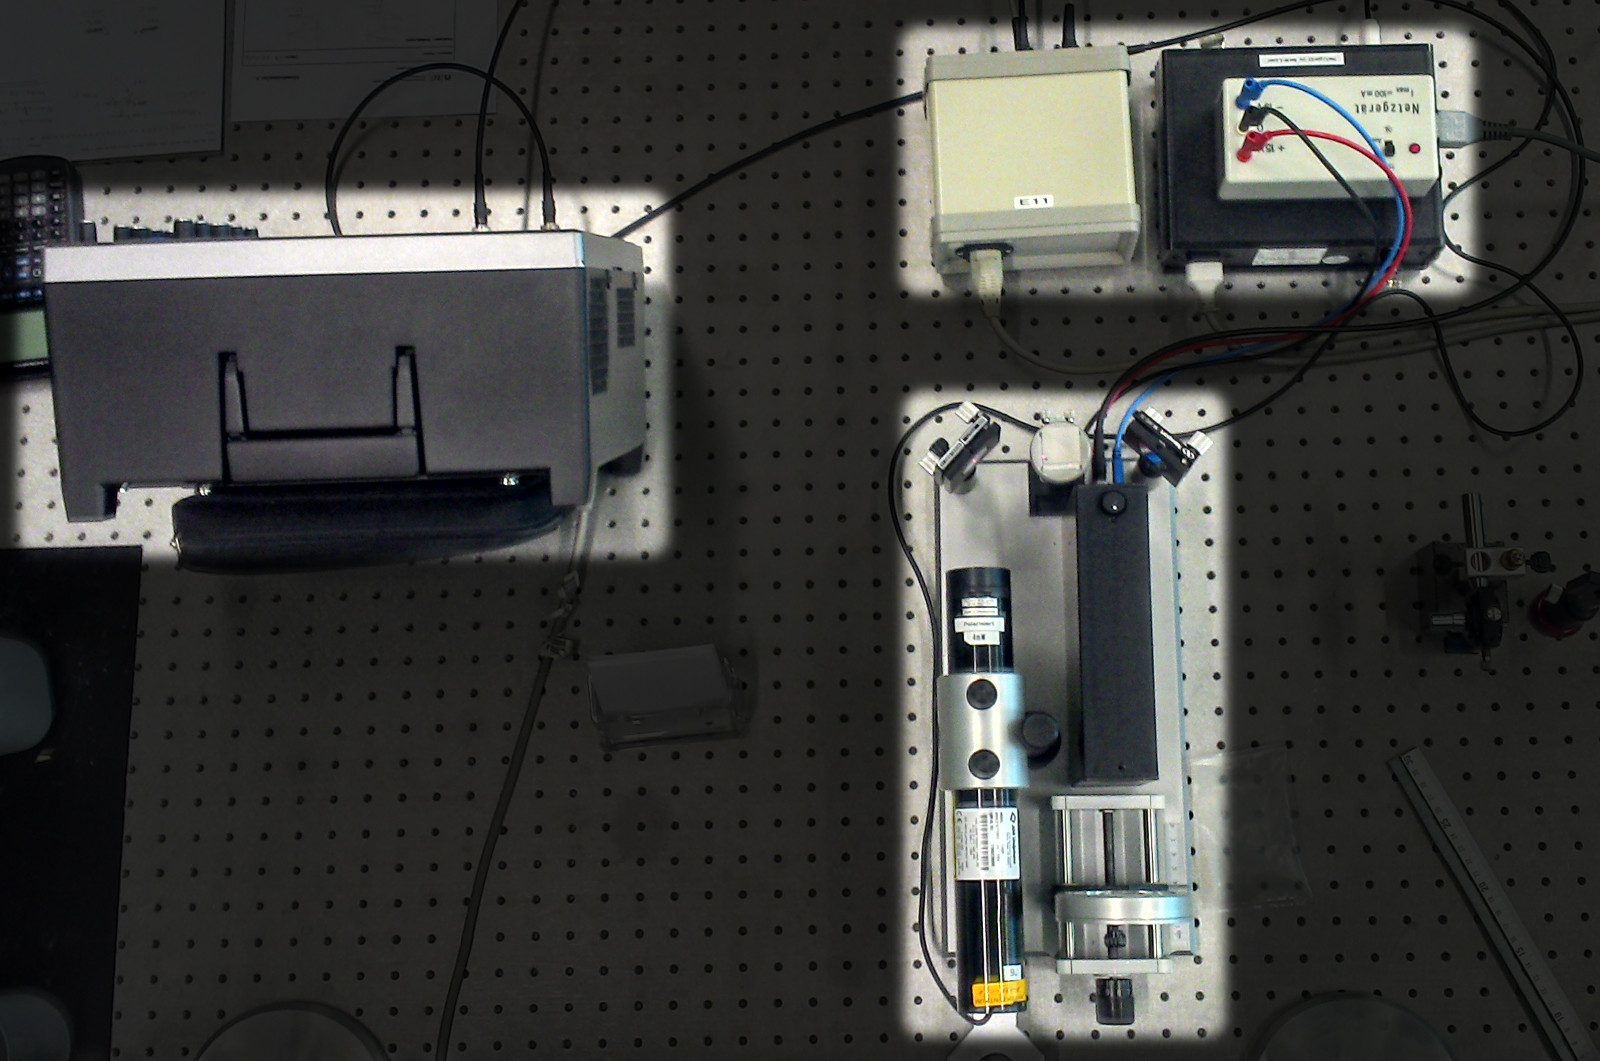
\includegraphics[width=300mm]{images/versuchsanordnung.jpeg}};

        % bounding box
        \draw[green] (0mm,0mm) rectangle (300mm,199mm);

        \node[white] at (40mm,140mm) {\Large{Oszilloskop}};

        \node[white] at (160mm,50mm) {\Large{Laser}};

        \node[white] at (160mm,120mm) {\Large{Spiegel}};

        \draw[cyan] (225mm,30mm) -- (234mm,30mm);
        \node[white] at (245mm,30mm) {\Large{Linse $L_1$}};

        \draw[cyan] (210mm,80mm) -- (234mm,80mm);
        \node[white] at (250mm,80mm) {\Large{\parbox{30mm}{\raggedright Geh\"ause mit \\Photomultiplier,\\ Blende und Linse $L_2$}}};

        \draw[cyan] (225mm,120mm) -- (234mm,120mm);
        \node[white] at (245mm,120mm) {\Large{Spiegel}};

        \node[black] at (195mm,175mm) {\Large{Bandpassfilter}};

        \node[white] at (235mm,157.5mm) {\Large{Netzger\"ate}};
    \end{scope}
\end{tikzpicture}
}
    \caption{%
        Versuchsanordnung, Vogelperspektive. Anordnung ist gr\"osstenteils mit
        dem Schema aus Abbildung \ref{fig:versuchsanordnung:schema} identisch.
    }
    \label{fig:versuchsanordnung:birdseye}
\end{figure}

\begin{figure}[h!t]
    \centering
    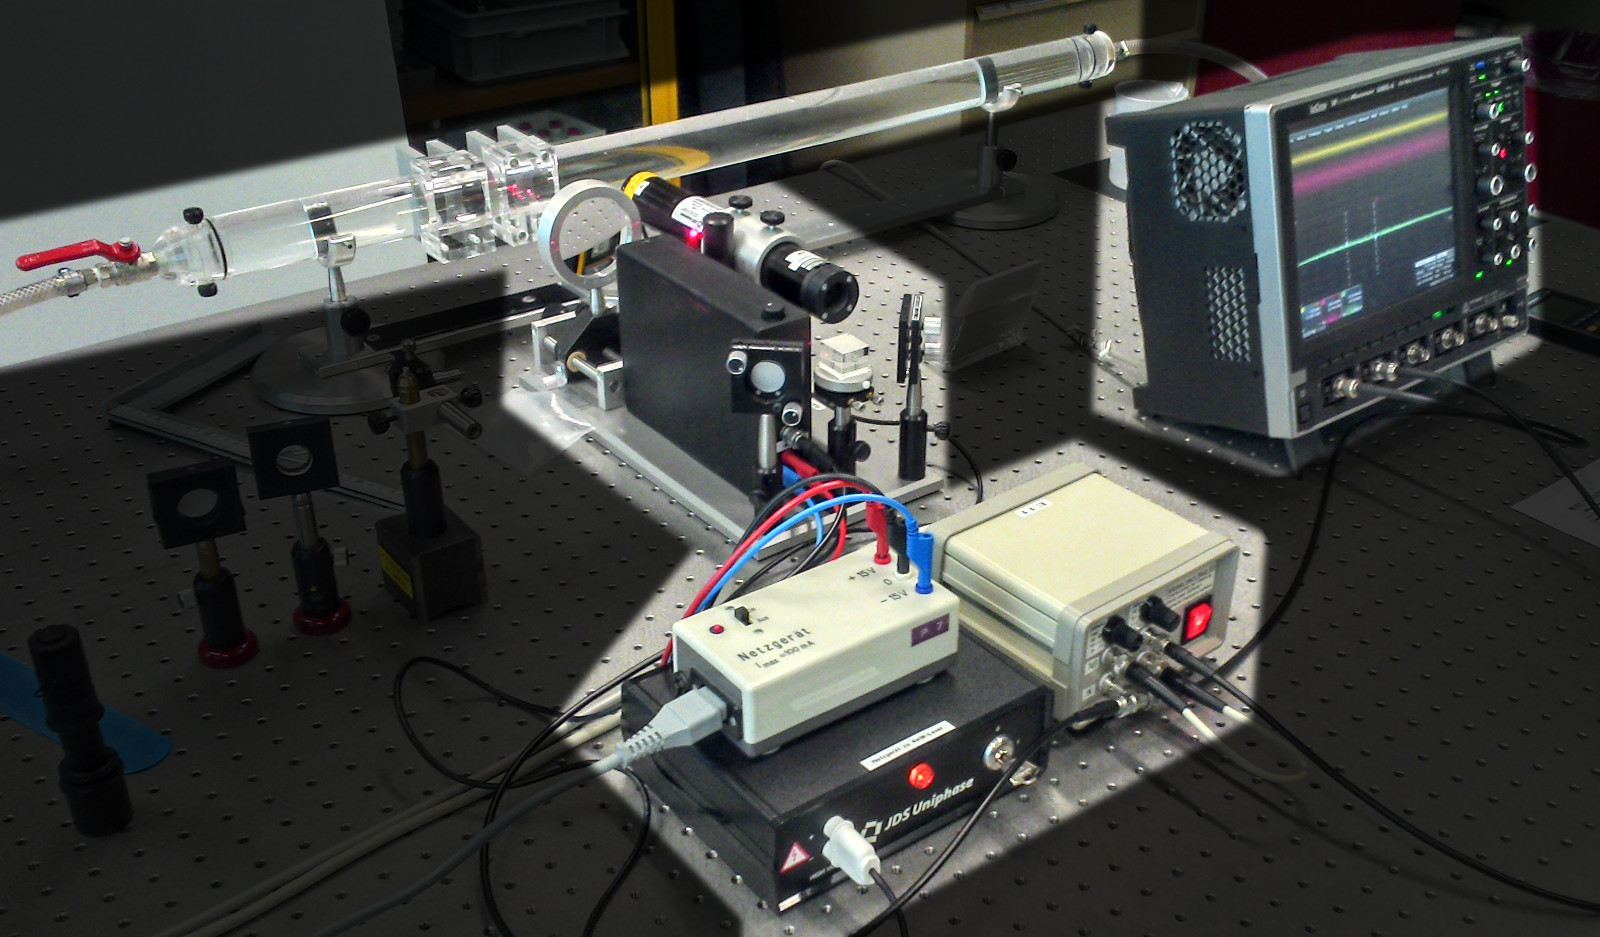
\includegraphics[width=.67\textwidth]{images/versuchsanordnung2.jpeg}
    \caption{%
        Versuchsanordnung,   andere   Perspektive. Messleitung   Sichtbar   im
        Hintergrund.
    }
    \label{fig:versuchsanordnung:perspective}
\end{figure}

Grunds\"atzlich  folgt   der  Versuchsaufbau  den  in   den  Arbeitsgrundlagen
beschriebenen    Angaben. Die   gesamte    Anordnung   ist    schematisch   in
Abbildung     \ref{fig:versuchsanordnung:schema}    dargestellt,     Abbildung
\ref{fig:versuchsanordnung:birdseye}  ist   die  entsprechende  fotographische
Dokumentation.  Abbildung  \ref{fig:versuchsanordnung:perspective} zeigt einen
anderen Blickwinkel auf die Apparaturen.

Um \"Uberlastung  durch Umgebungslicht zu verhindern,  ist der Photomultiplier
zusammen mit der Blende und der Linse $L_2$ in einem Geh\"ause eingelassen. Um
die Blende einzustellen und die Lage der Laserstrahlen zu \"uberpr\"ufen, kann
dieses  abgenommen  werden,  es  sollte aber  bei  Aktivierung  des  Detektors
montiert sein. Der Detektor  wird zwar nicht sofort zerst\"ort,  falls er ohne
Geh\"ause  eingeschaltet  wird,  der  Vorgang ist  aber  der  Lebensdauer  des
Ger\"ats nicht zutr\"aglich.

Das Geh\"ause kann in den Abbildungen \ref{fig:versuchsanordnung:birdseye} und
\ref{fig:versuchsanordnung:perspective} gesehen werden.


% ---------------------------------------------------------------------------- $
\clearpage
\subsection{Ger\"ate}
\label{subsec:messgerate}
% ---------------------------------------------------------------------------- $

\begin{table}[h!t]
    \centering
    \caption{Ger\"ateliste}
    \begin{tabular}{ll}
        \toprule
        \textsc{Ger\"at}
        & \textsc{Typ}
        \\

        \midrule

        Oszilloskop
        & LeCroy WaveRunner 64MXi-A
        \\

        Laser
        & JDS Uniphase 1122P, \SI{4}{\milli\watt}, polarisiert, $\lambda = \SI{632,8}{\nano\meter}$
        \\

        Pumpe
        & \SI{0.5}{\liter\per\minute} bis \SI{7.5}{\liter\per\minute} %TODO: modell
        \\

        Durchflussmesser
        & %TODO
        \\

        Detektor
        & Hamamatsu H9656-02 Photomultiplier
        \\

        Linse $L_1$
        & %TODO
        \\

        Linse $L_2$
        & \\

        Messleitung
        & Plexiglasrohr, Innendurchmesser \SI{40 \pm 0.5}{\milli\meter}
        \\

        Bandpassfilter
        & Tiefpass: \SI{3}{\kilo\hertz} bis \SI{300}{\kilo\hertz}, Hochpass: \SI{0.3}{\kilo\hertz} bis \SI{30}{\kilo\hertz}
        \\

        \bottomrule
    \end{tabular}
\end{table}

% ---------------------------------------------------------------------------- $
\clearpage
\subsection{Erwartete Reynoldszahlen und Signalfrequenzen}
\label{subsec:expectations}
% ---------------------------------------------------------------------------- $

Anhand der zur Verf\"ugung stehenden Leistung  der Pumpe und der Geometrie der
Apparatur kann an dieser Stelle  bereits abgesch\"atzt werden, welcher Bereich
f\"ur die Reynoldszahl ungef\"ahr abdeckbar sein wird. Zur Erinnerung:

\begin{equation}
    \label{eq:reynolds1}
    \mathit{Re} = \frac{\rho \cdot v_{\mathrm{m}} \cdot L}{\eta}
\end{equation}

Umrechnung der Durchflussraten in \si{\cubic\meter\per\second}:
\begin{align}
    \label{eq:Q:siconform}
    \dot{V}_{\mathrm{min}} = \SI{0.5}{\liter\per\minute} = \SI{8.3e-6}{\cubic\meter\per\second}
    \\
    \dot{V}_{\mathrm{max}} = \SI{7.5}{\liter\per\minute} = \SI{125e-6}{\cubic\meter\per\second}
\end{align}

Der Querschnitt des Rohres:
\begin{equation}
    \label{eq:cross_section}
    A = \pi \cdot R^2 = \SI{0.00126}{\meter\squared}
\end{equation}

Daraus lassen sich nun die mittleren Geschwindigkeiten f\"ur die schw\"achste
und st\"arkste Pumpeneinstellung bestimmen:
\begin{align}
    \label{eq:min_max_speed}
    v_{\mathrm{m,min}} = \frac{\dot{V}_{\mathrm{min}}}{A} = \SI{0.0066}{\meter\per\second}
    \\
    v_{\mathrm{m,max}} = \frac{\dot{V}_{\mathrm{max}}}{A} = \SI{0.099}{\meter\per\second}
\end{align}

Womit man f\"ur die Reynoldszahlen er\"alt:
\begin{align}
    \label{eq:reynolds:range}
    Re_{\mathrm{min}} = \frac{\rho \cdot v_{\mathrm{m,min}} \cdot 2R}{\eta} = 264
    \\
    Re_{\mathrm{max}} = \frac{\rho \cdot v_{\mathrm{m,max}} \cdot 2R}{\eta} = 3960
\end{align}

\begin{conditions}
    \rho & \SI{1000}{\kilo\gram\per\cubic\meter} \\
    R    & \SI{20}{\milli\meter} \\
    \eta & \SI{1}{\milli\pascal\second} (\emph{Quelle:} Kuchling, Tabelle 6)
\end{conditions}

Ebenfalls    lassen    sich     mit    den    errechneten    Geschwindigkeiten
$v_{\mathrm{m,min}}$ und  $v_{\mathrm{m,max}}$ ungef\"ahre Aussagen zu  den zu
erwartenden  Signalfrequenzen machen. Nat\"urlich  werden die  Frequenzen noch
davon abweichen, abh\"angig  davon, ob man gerade ein  Teilchen mit h\"ohrerer
oder  tieferer Geschwindigkeit  gemessen hat. Es  geht hier  lediglich um  die
Gr\"ossenordnung, sodass der Bandpassfilter jeweils korrekt eingestellt werden
kann. Es wurde mit $\varphi = \SI{30}{\degree}$ gerechnet.

\begin{align}
    \label{eq:expected_freqs}
    \Delta\,f_{\mathrm{min}} &= \frac{2\sin\left(\frac{\varphi}{2}\right) \cdot v}{\lambda} = \SI{10}{\kilo\hertz} \\
    \Delta\,f_{\mathrm{max}} &= \frac{2\sin\left(\frac{\varphi}{2}\right) \cdot v}{\lambda} = \SI{156}{\kilo\hertz}
\end{align}


% ---------------------------------------------------------------------------- $
\clearpage
\subsection{Ablauf}
\label{subsec:ablauf}
% ---------------------------------------------------------------------------- $

Wie  erw\"ahnt,  ist eine  korrekte  Justierung  dieses Versuches  f\"ur  eine
erfolgreiche  Durchf\"uhrung von  grosser Wichtigkeit. Sie  beanspruchte einen
betr\"achtlichen  Teil  der  zur   Verf\"ugung  stehenden  Zeit  (beinahe  die
H\"alfte) und soll hier entsprechend auch gut dokumentiert werden.

Die Krux am Ganzen ist, dass  die Laserstrahlen sich sauber in der Messleitung
kreuzen und anschliessend korrekt in den Detektor gef\"uhrt werden.

Dazu wurden zuerst an den in Abbildung \ref{fig:justierung} mit blauen Kreuzen
markierten  Punkten die  H\"ohe  der Laserstrahlen  gemessen  und mittels  der
Spiegel (siehe auch  Abbildung \ref{fig:spiegel}) und der Linse  $L_1$ auf die
gleiche H\"ohe eingestellt (so gut als m\"oglich, dieses Verfahren alleine ist
noch nicht genau genug).

\begin{figure}[h!t]
    \centering
    \resizebox{.67\textwidth}{!}{\begin{tikzpicture}
    \begin{scope}[x={(0mm,300mm)},y={(0mm,185mm)},line width=1pt,cap=round,rotate=-90]
        % bounding box
        %\draw[black] (190mm,70mm) rectangle (245mm,140mm);

        % laser and cable
        \draw[black] (200mm,120mm) rectangle (205mm,85mm);

        % mirror 1
        \fill[black,rotate around={45:(197.5mm,126.25mm)}] (197.5mm,125mm) rectangle (207.5mm,127.5mm);

        % beam splitter
        \fill[blue!30]  (215mm,127.5mm) rectangle (220mm,132.5mm);
        \draw[black!50] (215.2mm,132.3mm) -- (219.8mm,127.7mm);
        %\node at (215mm,120mm) {\footnotesize{1}};

        % mirror 2
        \fill[black,rotate around={-45:(237.5mm,126.25mm)}] (227.5mm,125mm) rectangle (237.5mm,127.5mm);

        % housing around detector and L2
        \fill[black!20] (219mm,122mm) rectangle (231mm,100mm);


        % dispersed light below lenses
        \fill[red!30] (221mm,90mm) rectangle (229mm,99.75mm);
        \fill[red!30] (221mm,99.75mm) -- (225mm,113mm) -- (229mm,99.75mm);
        \fill[red!30] (225mm,113mm) -- (224.5mm,115mm) -- (225.5mm,115mm);

        % detector and power cable and signal cables
        \draw[black] (222.5mm,120mm) rectangle (227.5mm,115mm);

        % aperture
        \fill[black] (222.5mm,114mm) rectangle (224mm,113mm);
        \fill[black] (226mm,114mm) rectangle (227.5mm,113mm);

        % lens L2
        \fill[blue!30] (225.25mm,100.5mm) -- (225mm,98.75mm) arc[start angle=-90,delta angle=-30,radius=12.5mm]  -- cycle;
        \fill[blue!30] (224.75mm,100.5mm) -- (225mm,98.75mm) arc[start angle=-90,delta angle=30,radius=12.5mm] -- cycle;

        % lens L1
        \fill[blue!30] (224.75mm,88.75mm) -- (225mm,92mm) arc[start angle=90,delta angle=-30,radius=25mm] -- cycle;
        \fill[blue!30] (225.25mm,88.75mm) -- (225mm,92mm) arc[start angle=90,delta angle=30,radius=25mm]  -- cycle;

        % Laser beams
        % laser -> L1
        \draw[red] (202.5mm,120mm) -- (202.5mm,129.5mm) -- (217.5mm,129.5mm) -- (217.5mm,91mm);
        % L1 -> L1
        \draw[red] (217.5mm,88.75mm) -- (225mm,75mm) -- (232.5mm,88.75mm);
        % L1 -> beam splitter
        \draw[red] (232.5mm,91mm) -- (232.5mm,129.5mm) -- (217.5mm,129.5mm);
        % particle -> L1 (dispersion)
        \fill[red!30] (225mm,75mm) -- (229mm,88.75mm) -- (221mm,88.75mm);

        % forward beam, left
        \draw[blue,rotate around={45:(217.5mm,120mm)}] (216.5mm,120mm) -- (218.5mm,120mm);
        \draw[blue,rotate around={-45:(217.5mm,120mm)}] (216.5mm,120mm) -- (218.5mm,120mm);

        % forward beam, right
        \draw[blue,rotate around={45:(232.5mm,120mm)}] (231.5mm,120mm) -- (233.5mm,120mm);
        \draw[blue,rotate around={-45:(232.5mm,120mm)}] (231.5mm,120mm) -- (233.5mm,120mm);

        % forward beam, after L1, left
        \draw[blue,rotate around={45:(219.5mm,85mm)}] (218.5mm,85mm) -- (220.5mm,85mm);
        \draw[blue,rotate around={-45:(219.5mm,85mm)}] (218.5mm,85mm) -- (220.5mm,85mm);

        % forward beam, after L1, right
        \draw[blue,rotate around={45:(230.5mm,85mm)}] (229.5mm,85mm) -- (231.5mm,85mm);
        \draw[blue,rotate around={-45:(230.5mm,85mm)}] (229.5mm,85mm) -- (231.5mm,85mm);

        % backwards beam, left
        \draw[blue,rotate around={45:(221mm,95mm)}] (220mm,95mm) -- (222mm,95mm);
        \draw[blue,rotate around={-45:(221mm,95mm)}] (220mm,95mm) -- (222mm,95mm);

        % backwards beam, right
        \draw[blue,rotate around={45:(229mm,95mm)}] (228mm,95mm) -- (230mm,95mm);
        \draw[blue,rotate around={-45:(229mm,95mm)}] (228mm,95mm) -- (230mm,95mm);
    \end{scope}
\end{tikzpicture}
}
    \caption{%
        Referenzpunkte f\"ur Kalibrierung (blau markiert)
    }
    \label{fig:justierung}
\end{figure}

Anschliessend wurde
%TODO: Instrument
benutzt,   um   die   beiden   Laserstrahlen   auf   eine   Wand   gegen\"uber
der   Versuchsanordnung  zu   projizieren. Dies   erm\"oglichte  eine   exakte
Zusammenf\"uhrung  der Laserstrahlen. Danach  wurde  sichergestellt, dass  die
Streuungen und Reflexionen der Strahlen,  welche zur\"uck in Richtung Detektor
gingen,  alle  auf  gleicher  H\"ohe   lagen,  indem  H\"ohe  und  Winkel  der
Messleitung korrekt eingestellt wurden. Abbildung \ref{fig:lensL1} zeigt diese
Strahlen vor ihrer Justierung.

Letzlich wurde \"uberpr\"uft, dass  der Kreuzungspunkt der gestreuten Strahlen
genau in der Blende (sichtbar in Abbildung \ref{fig:versuchsanordnung:blende})
lag, und die Blende so weit als m\"oglich geschlossen.

\begin{figure}[h!t]
    \centering
    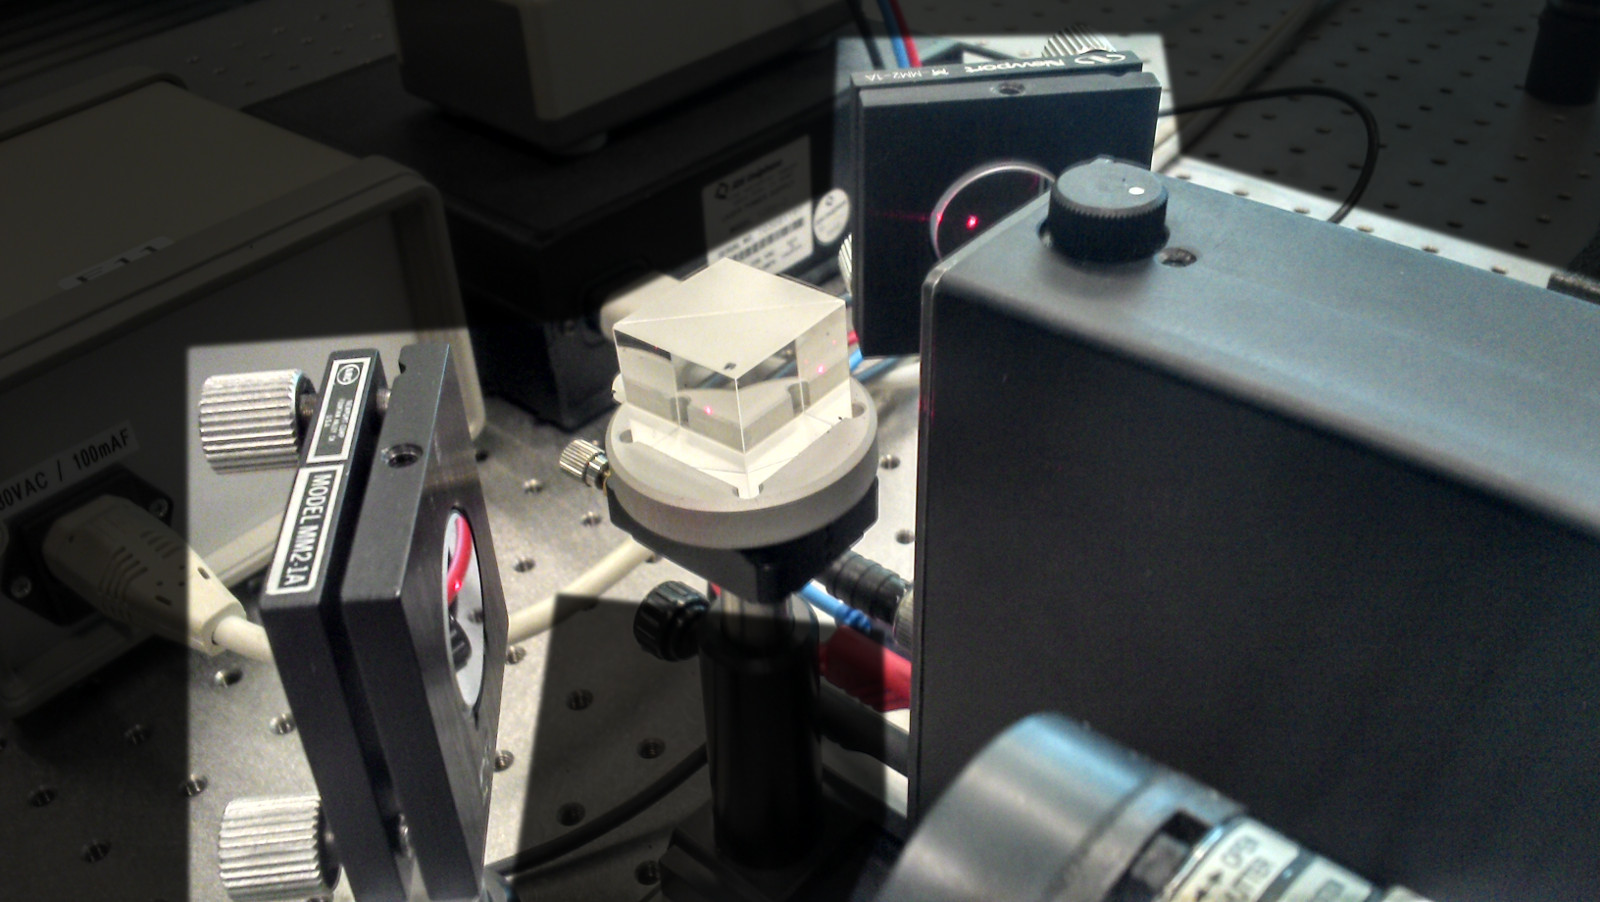
\includegraphics[width=.67\textwidth]{images/spiegel.jpeg}
    \caption{%
        Die beiden Spiegel und der Strahlteiler. Die Spiegel k\"onnen vestellt
        werden, um die Verl\"aufe der Strahlen aufeinander abzustimmen.
    }
    \label{fig:spiegel}
\end{figure}


\begin{figure}[h!t]
    \centering
    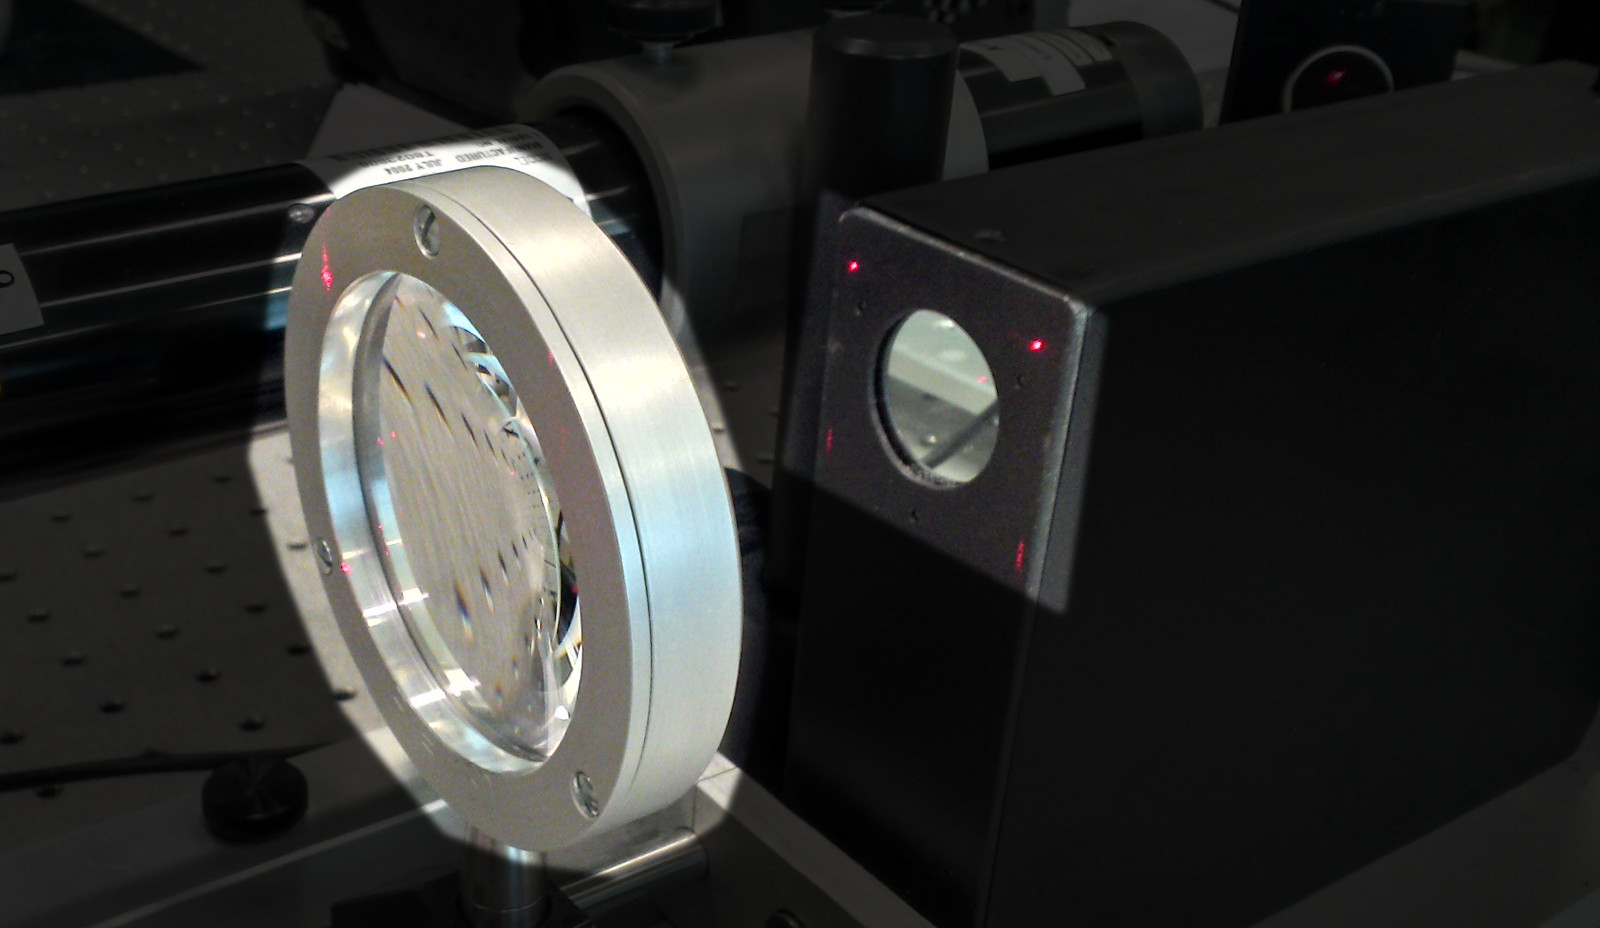
\includegraphics[width=.67\textwidth]{images/linse.jpeg}
    \caption{%
        Die  Linsen  $L_1$ (links,  gross)  und  $L_2$ (rechts,  im  schwarzen
        rechteckigen  Rahmen). Ebenfalls  sichtbar   sind  einige  Reflexionen
        der  Laserstrahlen am  Rahmen  von $L_2$,  bevor  sie justiert  worden
        sind. Nach der Justierung liegen alle vier Punkte auf gleicher H\"ohe.
    }
    \label{fig:lensL1}
\end{figure}

\begin{figure}[h!t]
    \centering
    \resizebox{.67\textwidth}{!}{\begin{tikzpicture}
    \begin{scope}[x={(0mm,300mm)},y={(0mm,199mm)},line width=1pt,cap=round]
        \node[anchor=south west,inner sep=0mm] at (0mm,0mm) {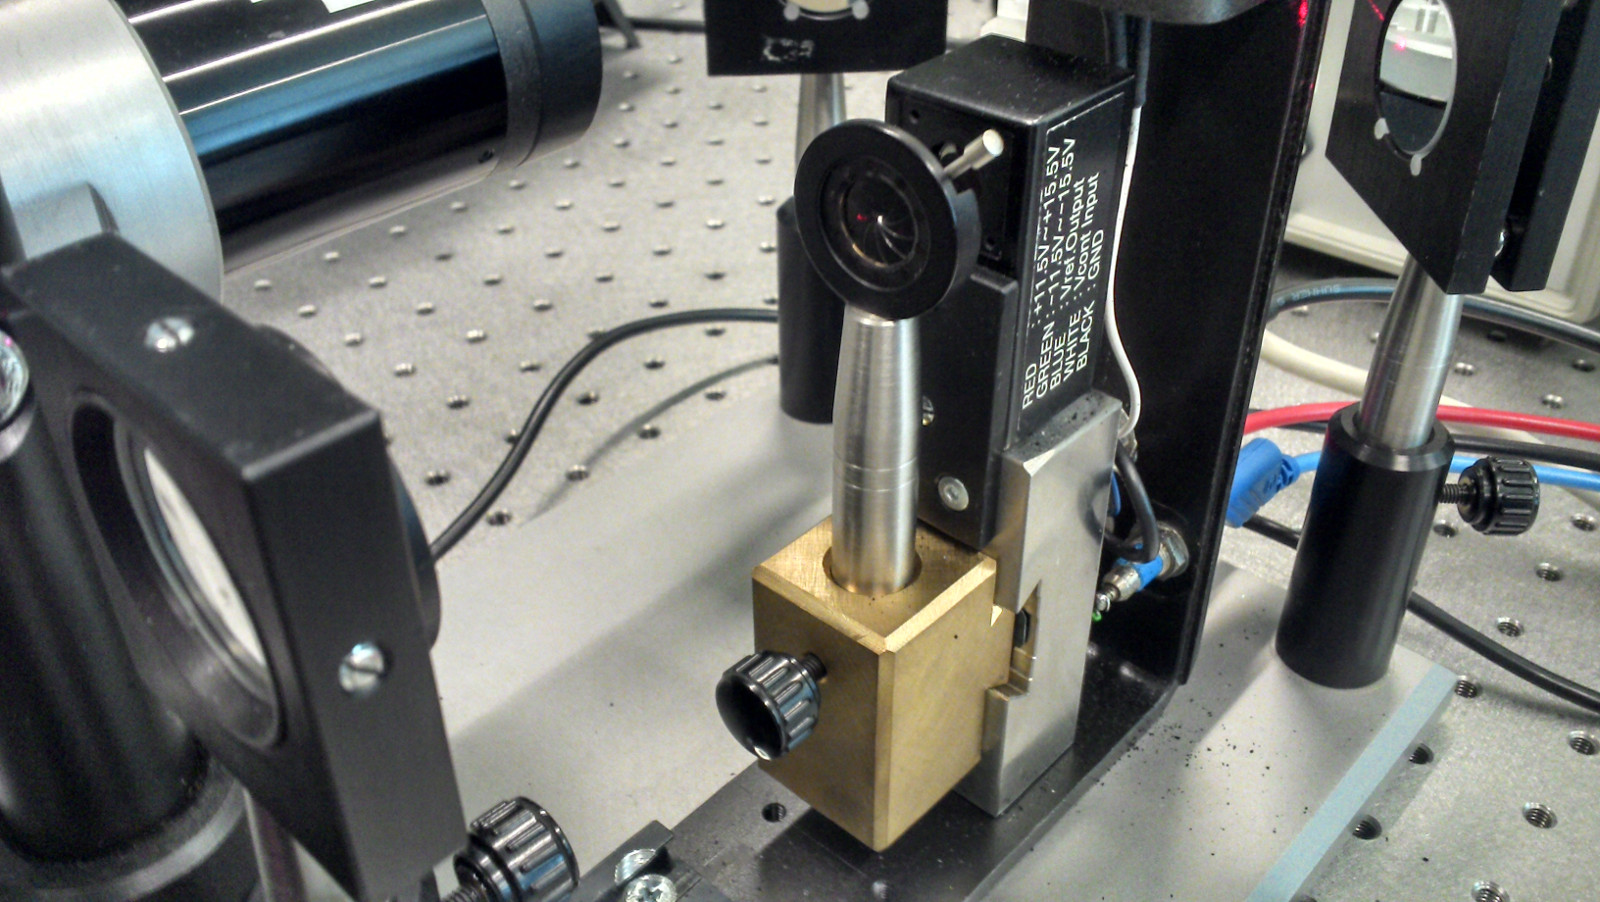
\includegraphics[width=300mm]{images/blende.jpeg}};

        %\draw[cyan] (210mm,80mm) -- (234mm,80mm);
        %\node[white] at (250mm,80mm) {\Large{\parbox{30mm}{\raggedright Geh\"ause mit \\Photomultiplier,\\ Blende und Linse $L_2$}}};
    \end{scope}
\end{tikzpicture}
}
    \caption{%
        Linse  $L_2$, Blende  und Photomultiplier. Die  Blende kann  verstellt
        werden,  um  m\"oglichst  nur  das  vom Str\"omungsteilchen  gestreute
        Laserlicht in den Photomultiplier zu lassen.
    }
    \label{fig:versuchsanordnung:blende}
\end{figure}

Die  Kreuzung  der   Laserstrahlen  in  der  Messleitung   kann  in  Abbildung
\ref{fig:laserkreuzung} gesehen werden.

\begin{figure}[h!t]
    \centering
    \resizebox{.67\textwidth}{!}{\begin{tikzpicture}
    \begin{scope}[x={(0mm,300mm)},y={(0mm,100mm)},line width=1pt,cap=round]
        \node[anchor=south west,inner sep=0mm] at (10mm,10mm) {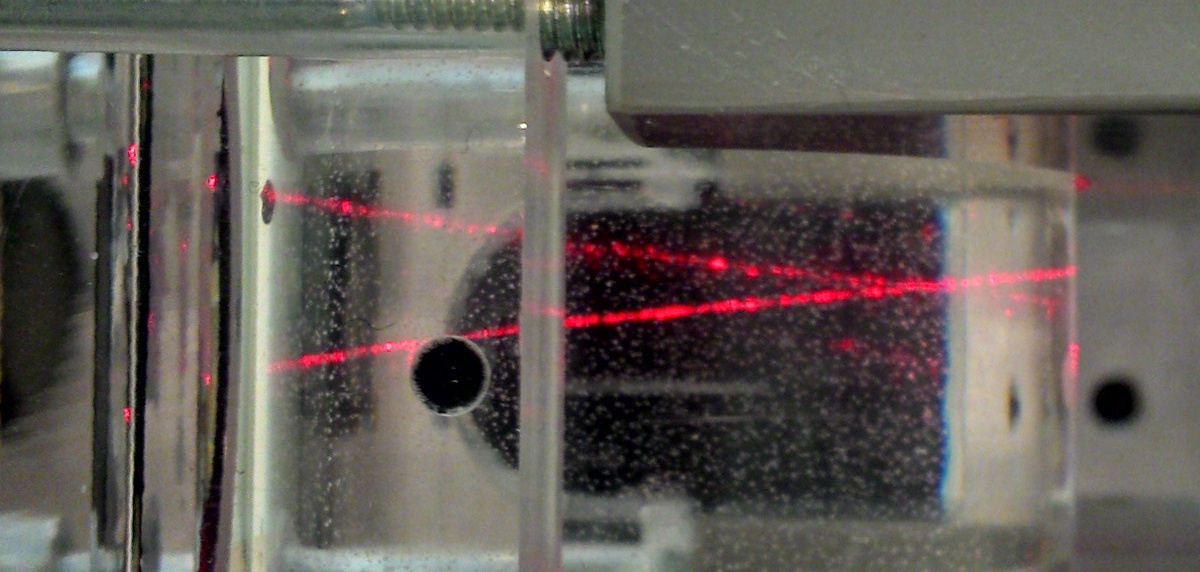
\includegraphics[width=260mm]{images/beams.jpeg}};

        \draw[-latex,line width=2pt] (5mm,30mm) -- (5mm,110mm);
        \node[rotate=90] at (1mm,65mm) {\huge{Wasserstr\"omung}};

        \draw[-latex,line width=2pt] (65mm,5.5mm) -- (230mm,5.5mm);
        \node at (150mm,0mm) {\huge{Einfallsrichtung Laserstrahlen}};
        %\draw[cyan] (210mm,80mm) -- (234mm,80mm);
        %\node[white] at (250mm,80mm) {\Large{\parbox{30mm}{\raggedright Geh\"ause mit \\Photomultiplier,\\ Blende und Linse $L_2$}}};
    \end{scope}
\end{tikzpicture}
}
    \caption{%
        Aufname      der     sich      kreuzenden     Strahlen      in     der
        Messleitung. Wasserstr\"omung   geht   von   unten  nach   oben,   die
        Laserstrahlen treffen von links auf die Messleitung.
    }
    \label{fig:laserkreuzung}
\end{figure}

Nachdem die Apparatur justiert war, wurden vier Messungen durchgef\"uhrt:

\begin{itemize}
    \item
        Eine experimentelle \"Uperpr\"ufung der Brennweite von Linse $L_1$,
    \item
        das  Verhalten  der  Str\"omungsgeschwindigkeit   auf  der  Achse  der
        Messleitung  bei Durchflussraten  zwischen \SI{0.5}{\liter\per\minute}
        und \SI{7.5}{\liter\per\minute},
    \item
        das  Geschwindigkeitsprofil   \"uber  den  gesamten   Querschnitt  der
        Messleitung bei \SI{0.5}{\liter\per\minute} (laminarer Fall) und
    \item
        das  Geschwindigkeitsprofil   \"uber  den  gesamten   Querschnitt  der
        Messleitung bei \SI{7.5}{\liter\per\minute} (turbulenter Fall).
\end{itemize}

Zur  Auswertung wurde  dabei das  Oszilloskop benutzt. Es  erhielt sowohl  das
ungefilterte Messsignal direkt from Photomultiplier (sehr verrauscht) wie auch
das gefilterte Signal aus dem Bandpassfilter.

Um  den  Bandpassfiter  korrekt  einstellen zu  k\"onnen,  musste  nat\"urlich
bekannt sein, in  welcher Gr\"ossenordnung sich die  zu erwartenden Frequenzen
ungef\"ahr befinden w\"urden.
%TODO: Frequency calculations

Das  Oszilloskop f\"uhrte  am  eingehenden  Zeitsignal eine  Fourier-Zerlegung
durch (unterstes Signal in Abbildung
% TODO: abbildung Oszi
).  In  diesem  Signal  wurden  dann mittels  der  beiden  Cursor  eine  obere
und  untere  Limite der  bei  einer  Einstellung (Position  des  Schnittpunkts
der  Laserstrahlen  in  der  Messleitung,  Flussgeschwindigkeit)  auftretenden
Frequenzen  abgelesen. Zur  Auswertung  wird  aus diesen  der  Mittelwert  mit
Unsicherheit gebildet (siehe Abschnitt.
%TODO Referenz
auf Seite
%TODO Referenz
).

Bei  \"andernden  Einstellungen musste  jeweils  darauf  geachtet werden,  den
Bandpass  entsprechend  anzupassen. Geht  dies   vergessen,  werden  zwar  die
Messresultate nicht  verf\"alscht, es  macht aber  das Erkennen  der gesuchten
Streu-Ereignisse zunehmend  schwierig oder verhindert sie  vollkommen, je nach
Frequenzbereich.


%TODO: Grunds\"atzlich: What happens when we do this? Might already have been explained
% in arbeitsgrundlagen.



% **************************************************************************** %
\clearpage
\section{Auswertung}
\label{sec:auswertung}
% **************************************************************************** %
% ---------------------------------------------------------------------------- %
\subsection{Versuch 3.1.1 -- Tr\"agheitsmoment $I_0$ des Pendels ohne Reiter}
\label{subsec:i0}
% ---------------------------------------------------------------------------- %

\begin{figure}[h!]
    \centering
    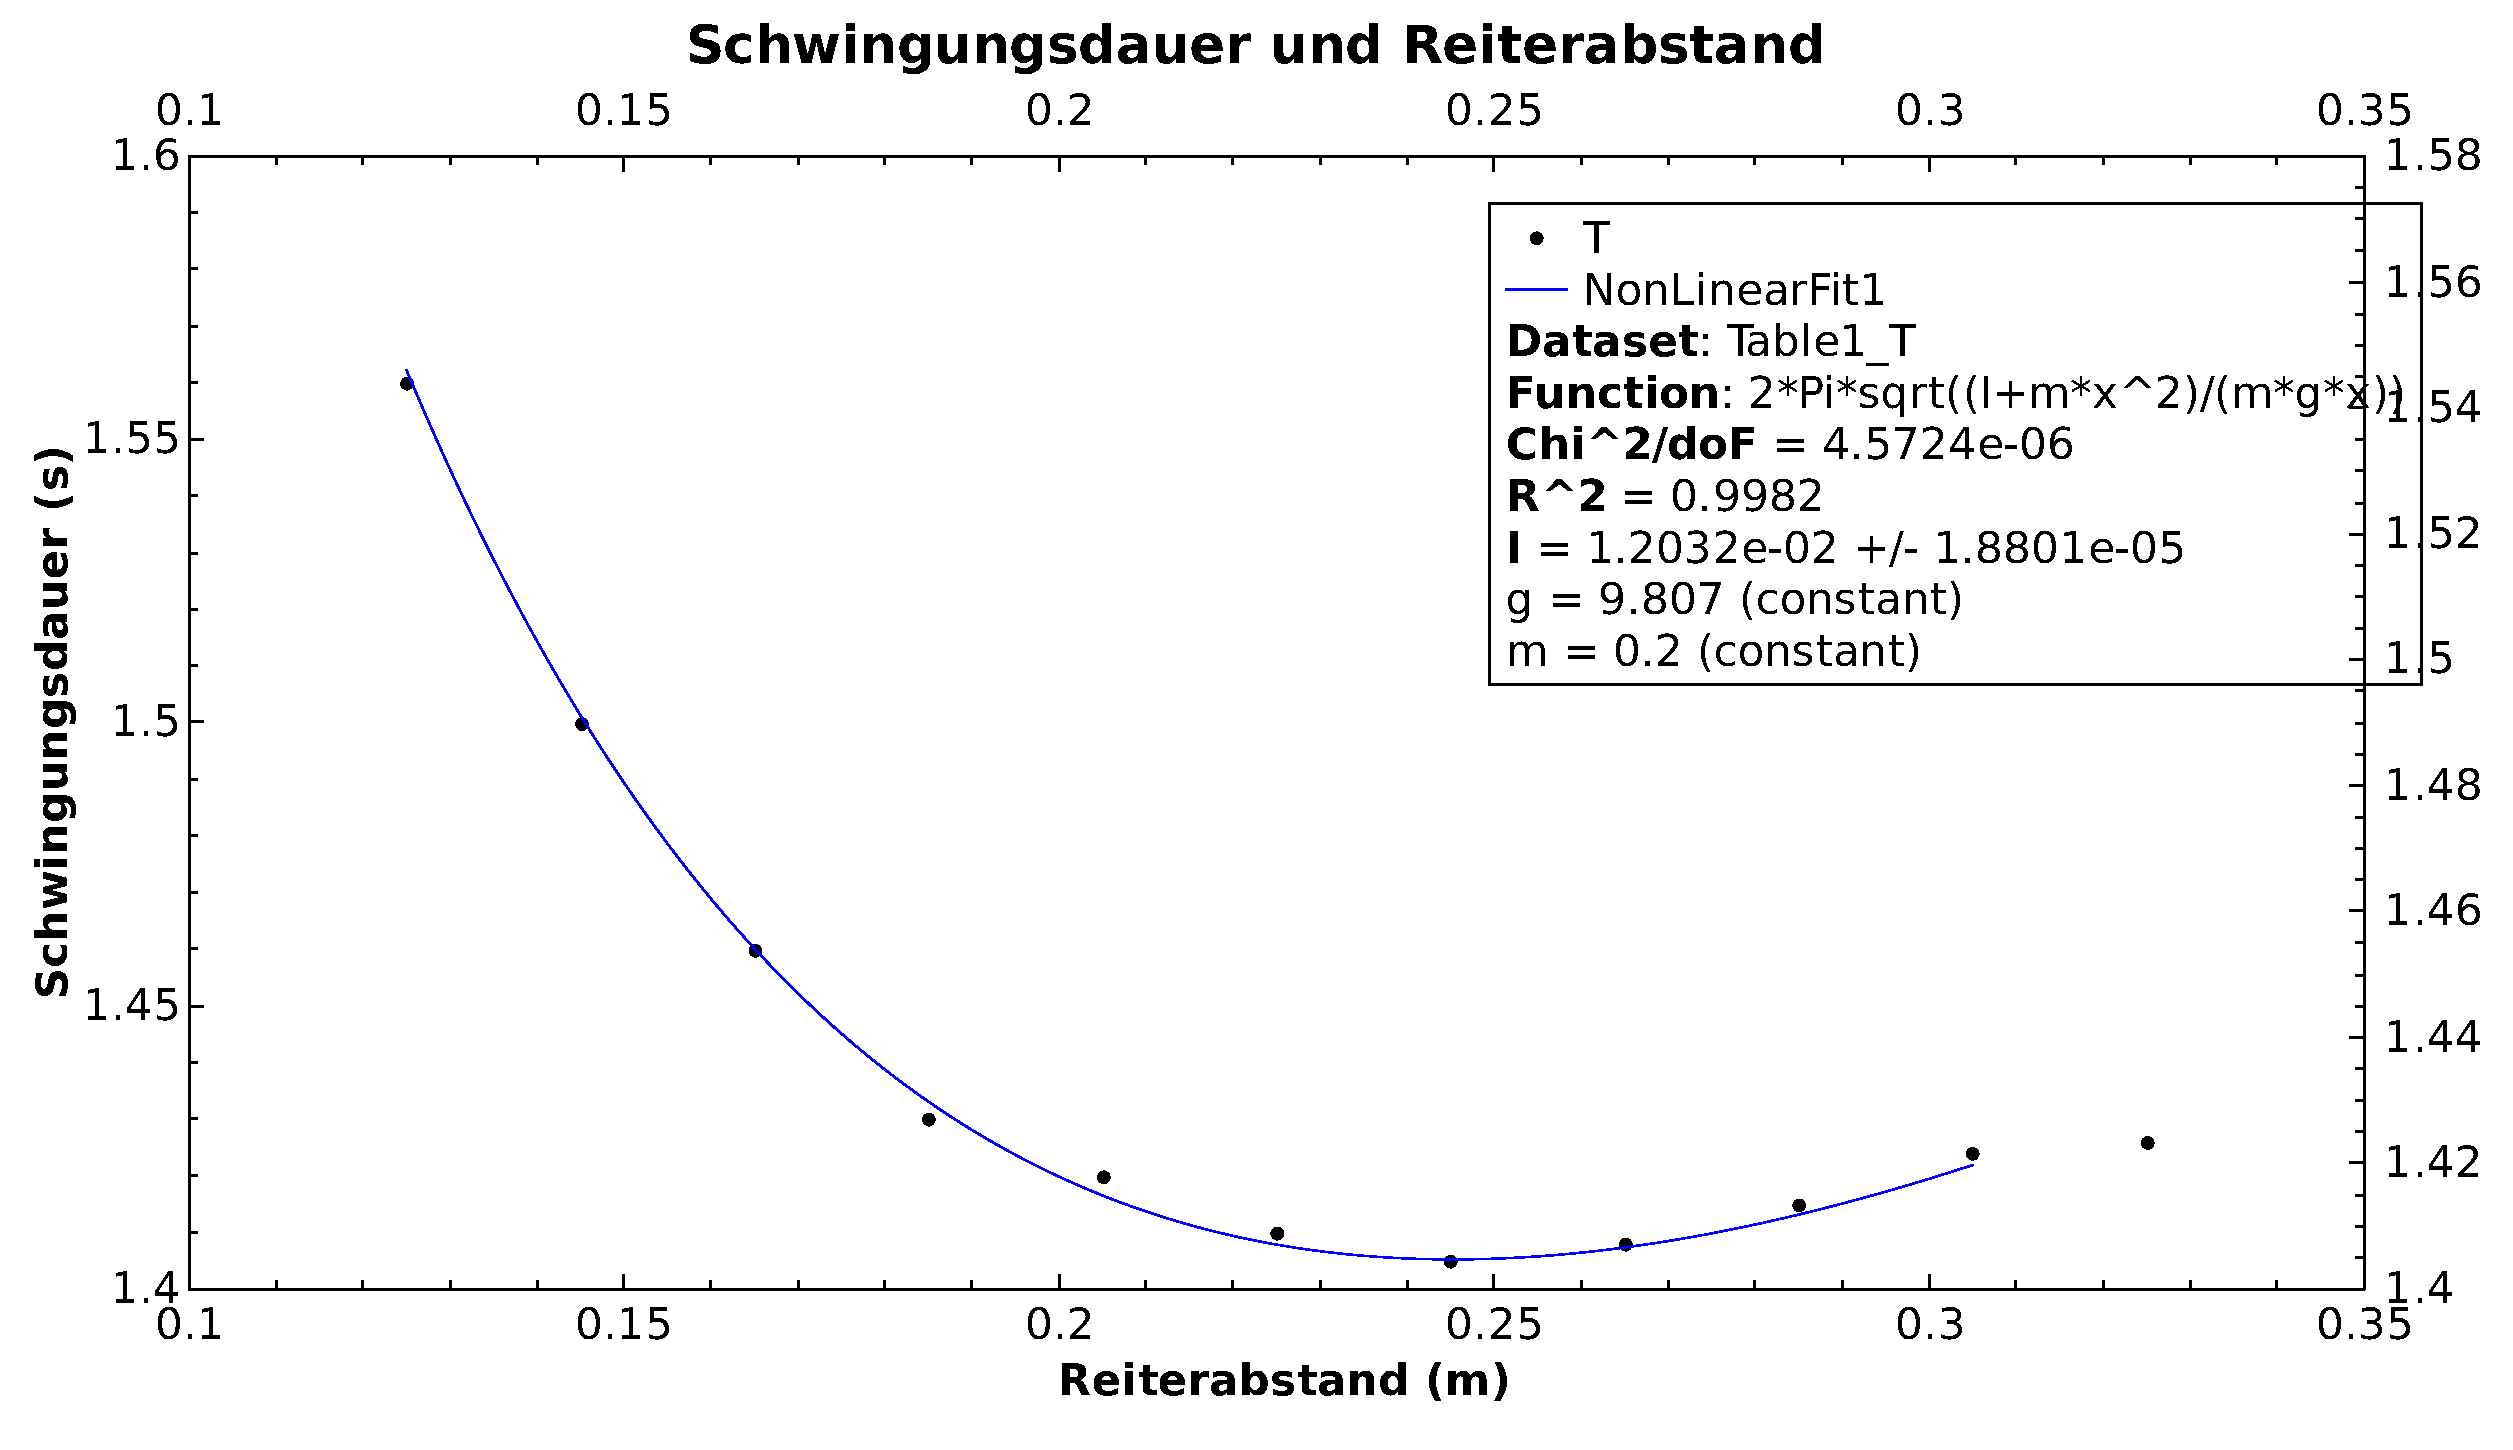
\includegraphics[width=\textwidth]{images/311.pdf}
    \caption{%
        Massentr\"agheitsmoment des Pendels ohne Reiter
    }
    \label{fig:pendelKonfigs}
\end{figure}

Die Messungen  wurden ausgef\"uhrt  mit einer Reitermasse  von \SI{200}{\gram}
und verschiedenen Abst\"anden. Der letzte Messpunkt bei \SI{325}{\milli\meter}
wurde  im  Fit nicht  ber\"ucksichtigt,  da  er  stark nach  einem  Ausreisser
aussieht.

Der Referenzwert aus der Versuchsanleitung f\"ur $I_0$ ist $\SI{1.16e-2}{\kilo\gram\meter\squared}$,
der mittels Fit ermittelte Wert betr\"agt $I_0  = \SI[separate-uncertainty = true]{12.032 \pm 0.018801}{\gram\meter\squared}$.


% ---------------------------------------------------------------------------- %
\clearpage
\subsection{Versuch 3.1.2 -- Schwingungsdauer in Funktion der Reitermasse}
\label{subsec:periodeReitermasse}
% ---------------------------------------------------------------------------- %

Im  Gegensatz zum  vorigen Versuch,  bei  dem die  Reitermasse als  Punktmasse
approximiert  wurde, sollte  gem\"ass Versuchsanleitung  das Tr\"agheitsmoment
des Reiters ab \SI{400}{\gram} ber\"ucksichtigt werden.

Da wir  in dieser Versuchsreihe  bis zu einer Reitermasse  von \SI{700}{\gram}
gemessen  haben, ist  es  naheliegend, eine  genauere Formel  herzuleiten. Ein
Problem beim  Fitten mit  QtiPlot in  diesem Fall, ist,  dass die  L\"ange des
Reiters mit  seiner Masse  variiert; man hat  also eigentlich  zwei Variablen,
welche sich  von Messung zu Messung  \"andern und in die  resultierende Formel
einfliessen sollten.

\begin{equation}
    T_0 = 2 \cdot \pi \cdot \sqrt{\frac{I_0 + I_{Reiter}}{m \cdot g \cdot a}}
\end{equation}

mit  $I_{Reiter}  =  I_{Zylinder} +  I_{Steineranteil}$. Mit  $I_{Zylinder}  =
\frac{m}{12} \cdot (  3 \cdot r^2 + h^2)$ und  $I_{Steineranteil} = m_{Reiter}
\cdot a^2$ (Quelle: Kuchling) ergibt dies:

\begin{equation}
    T_0 = 2 \cdot \pi \cdot \sqrt{\frac{I_0 + \frac{m_{Reiter}}{12} \cdot (3\cdot r^2 + h^2) + m_{Reiter} \cdot a^2}{m_{Reiter} \cdot g \cdot a}}
\end{equation}

Gl\"ucklicherweise  h\"angt  aber die  Masse  des  Reiters linear  von  seiner
L\"ange  ab (der  Durchmesser  aller Messproben  ist  identisch und  betr\"agt
\SI{34.4}{\milli\meter}); man hat also  nur einen Freiheitsgrad. Alles, was zu
tun bleibt, ist,  obige Gleichung in Funktion der  Zylinderl\"ange des Reiters
umzuschreiben, und den Fit mittels dieser Werte zu machen.

Dazu  wird  die   L\"angendichte  $\rho$  des  Reiters   als  neuer  Parameter
eingef\"uhrt, und  obige Funktion  umgeschrieben mit der  L\"ange $l_{Reiter}$
als  Funktionsparameter,   wobei  die  Reitermasse  dann   definiert  ist  als
$m_{Reiter} = \rho \cdot l_{Reiter}$:

\begin{equation}
    T_0 = 2 \cdot \pi \cdot \sqrt{\frac{I_0 + \frac{\rho \cdot l_{Reiter}}{12} \cdot (3\cdot r^2 + l_{Reiter}^2) + \rho \cdot l_{Reiter} \cdot a^2}{\rho \cdot l_{Reiter} \cdot g \cdot a}}
\end{equation}

Die verwendeten Parameter sind:
\begin{itemize}
    \item
        $\rho = \SI{6.667}{\kilo\gram\per\meter}$
    \item
        $l_{Reiter}$: Variable auf horizontaler Achse
    \item
        $r = \SI{17.2}{\milli\meter}$ (Radius des Reiters)
    \item
        $a = \SI{325}{\milli\meter}$ (Position des Mittelpunktes des Reiters)
    \item
        $g = \SI{9.807}{\meter\per\second\squared}$
\end{itemize}


Approximiert  man  den Reiter  als  Punktmasse  wie beim  vorherigen  Versuch,
ergibt   sich   das  Resultat   aus   Abbildung   \ref{fig:312a},  mit   einem
Massentr\"agheitsmoment von
$I_0  = \SI[separate-uncertainty = true]{11.362 \pm 0.39697}{\gram\meter\squared}$.
\begin{figure}[h!]
    \centering
    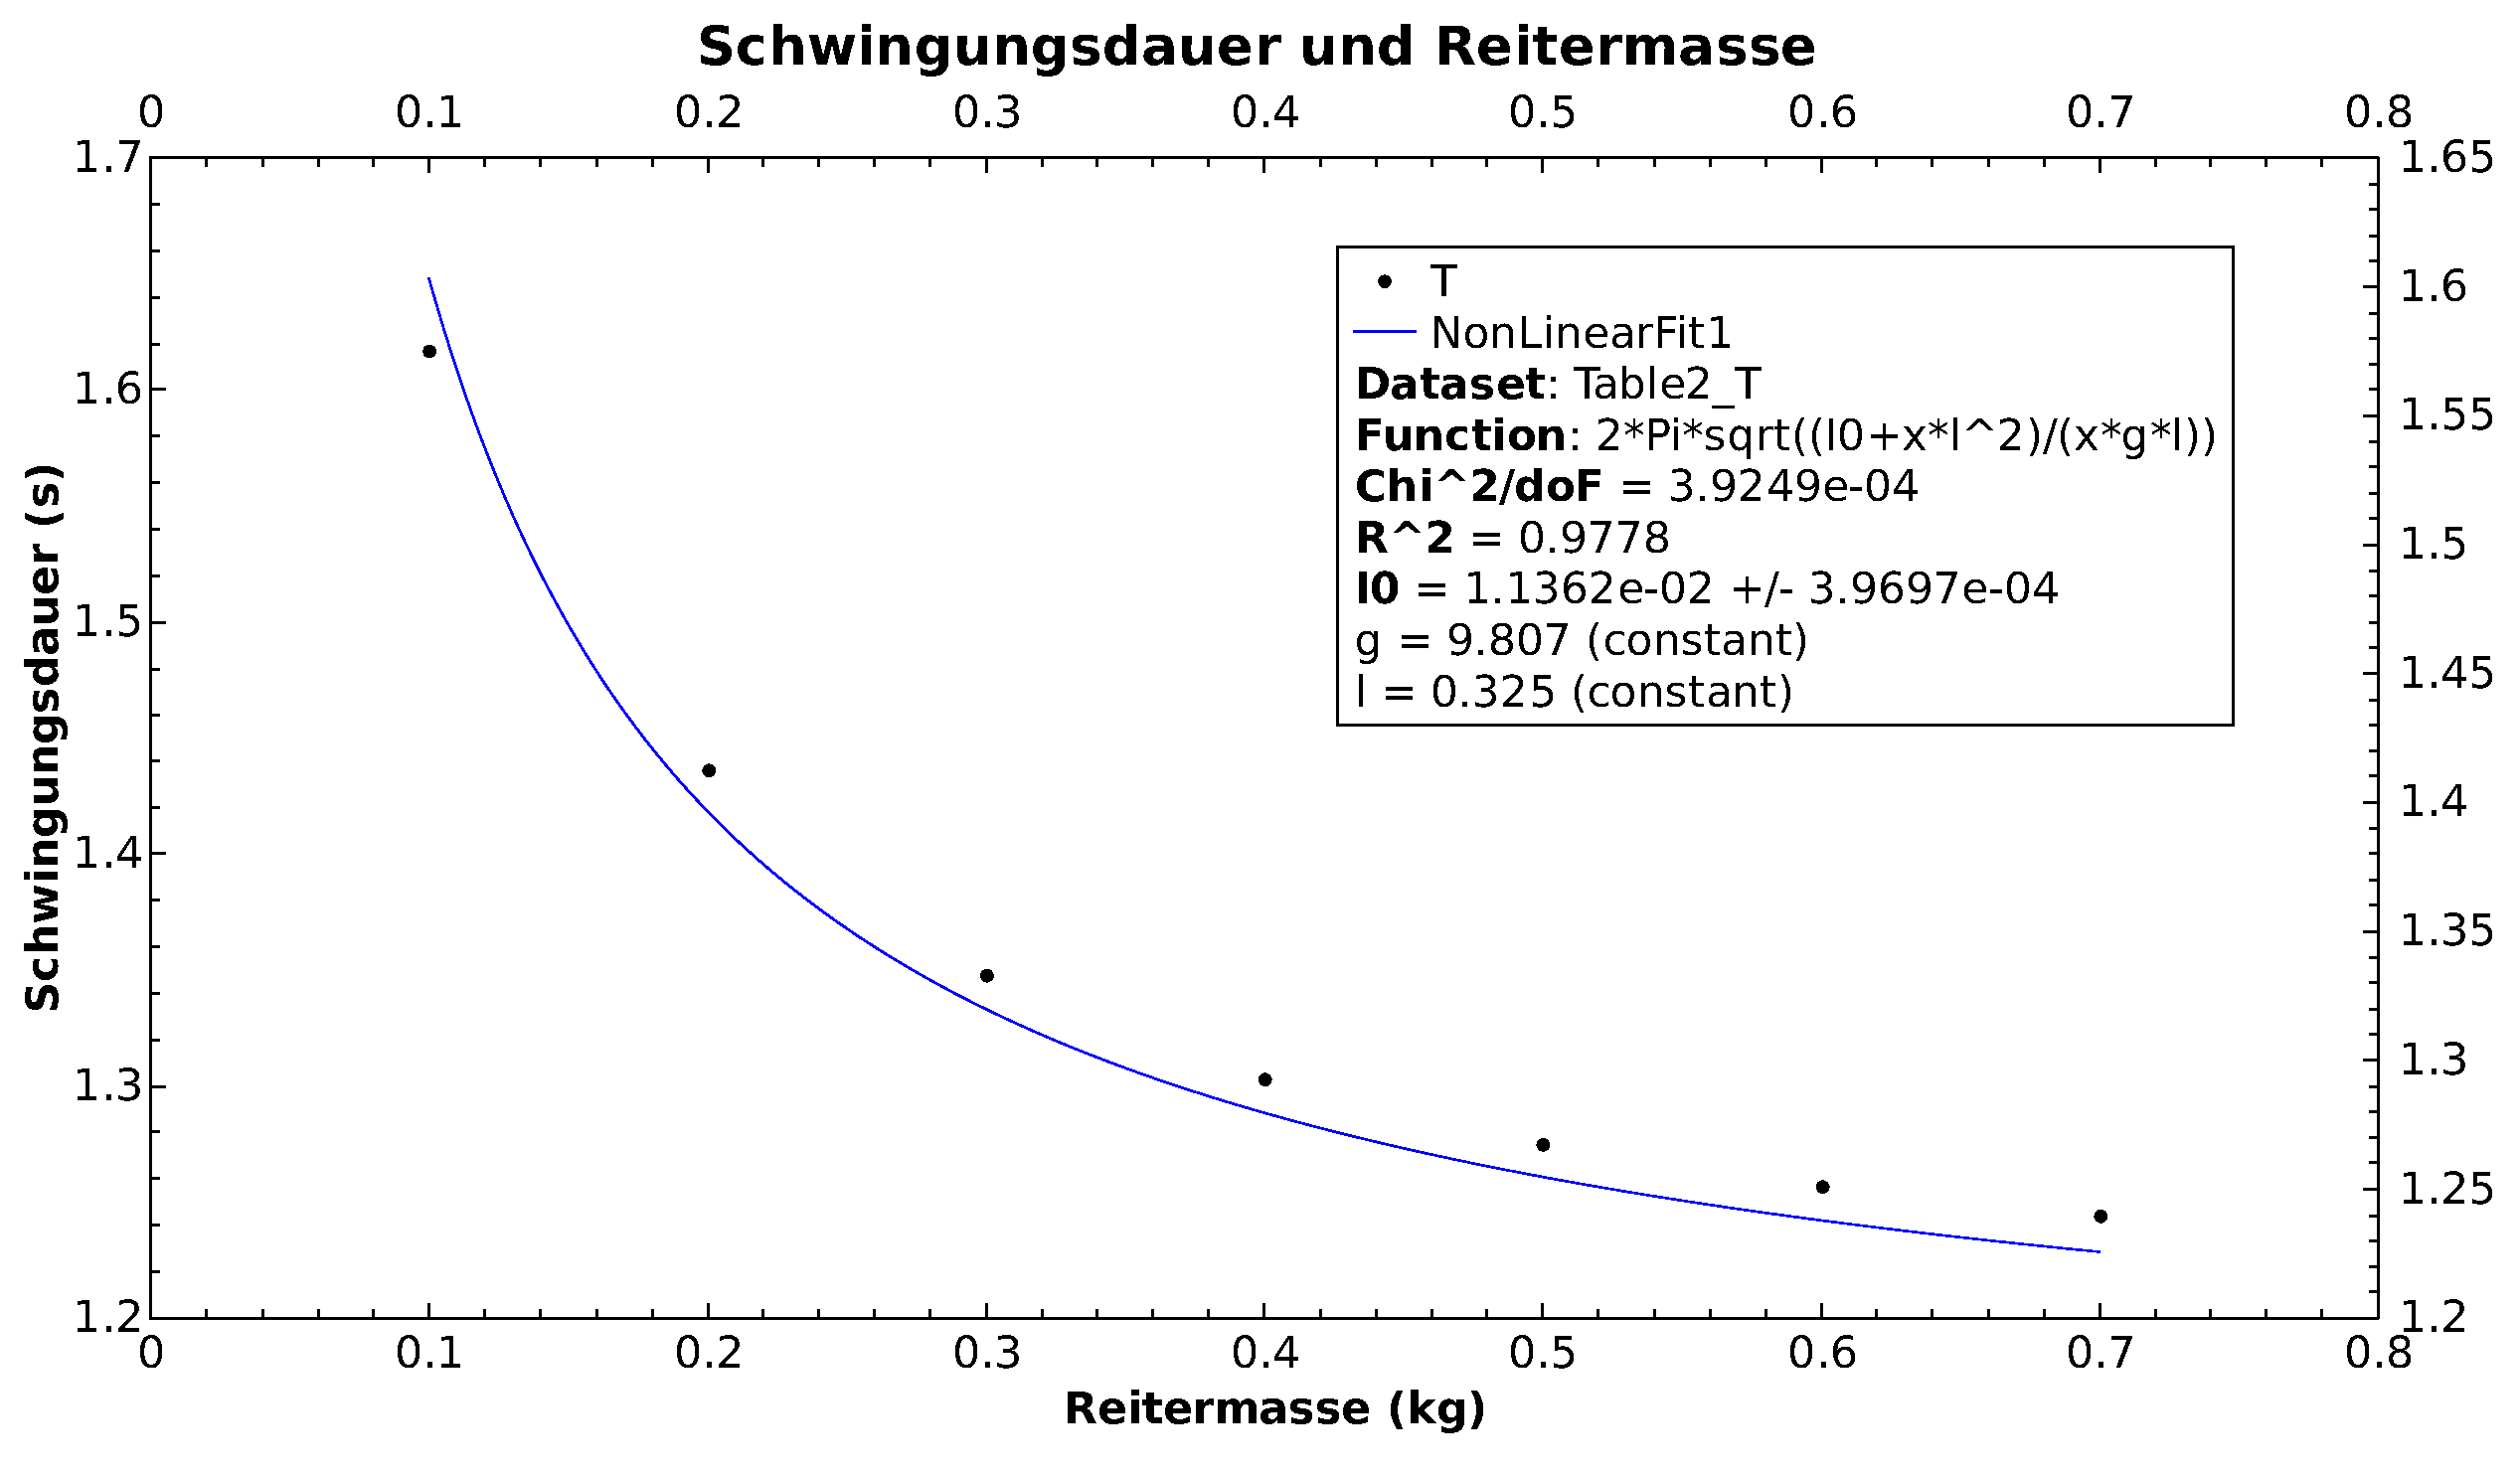
\includegraphics[width=\textwidth]{images/312.pdf}
    \caption{%
        Schwingungsdauer in Abh\"angigkeit der Reitermasse, gefitted \"uber Tr\"agheitsmoment. Abstand des Reiters war konstant \SI{325}{\milli\meter}.
    }
    \label{fig:312a}
\end{figure}

Wie man  in Abbildung  \ref{fig:312a} erkennen  kann, besteht  eine Abweichung
zwischen Fit  und Messwerten,  welche eine  zunehmende Tendenz  mit steigender
Reitermasse aufweist. Ich  f\"uhre das auf die  zunehmende Diskrepanz zwischen
der Ann\"aherung des Reiters als Punktmasse  mit $I_{Reiter} = m\cdot a^2$ und
der Modellierung als Zylinder inklusive Steiner-Anteil durch
$I_{Reiter} = \frac{m}{12}(3  \cdot r^2  + h^2) +  m \cdot a^2$.

Ber\"ucksichtigt  man die  Zylindrigkeit  des Reiters  und den  Steiner-Anteil
(siehe Abbildung \ref{fig:312b}), ergibt sich ein Massentr\"agheitsmoment von
$I_0  = \SI[separate-uncertainty = true]{11.297 \pm 0.36271}{\gram\meter\squared}$.

\begin{figure}[h!]
    \centering
    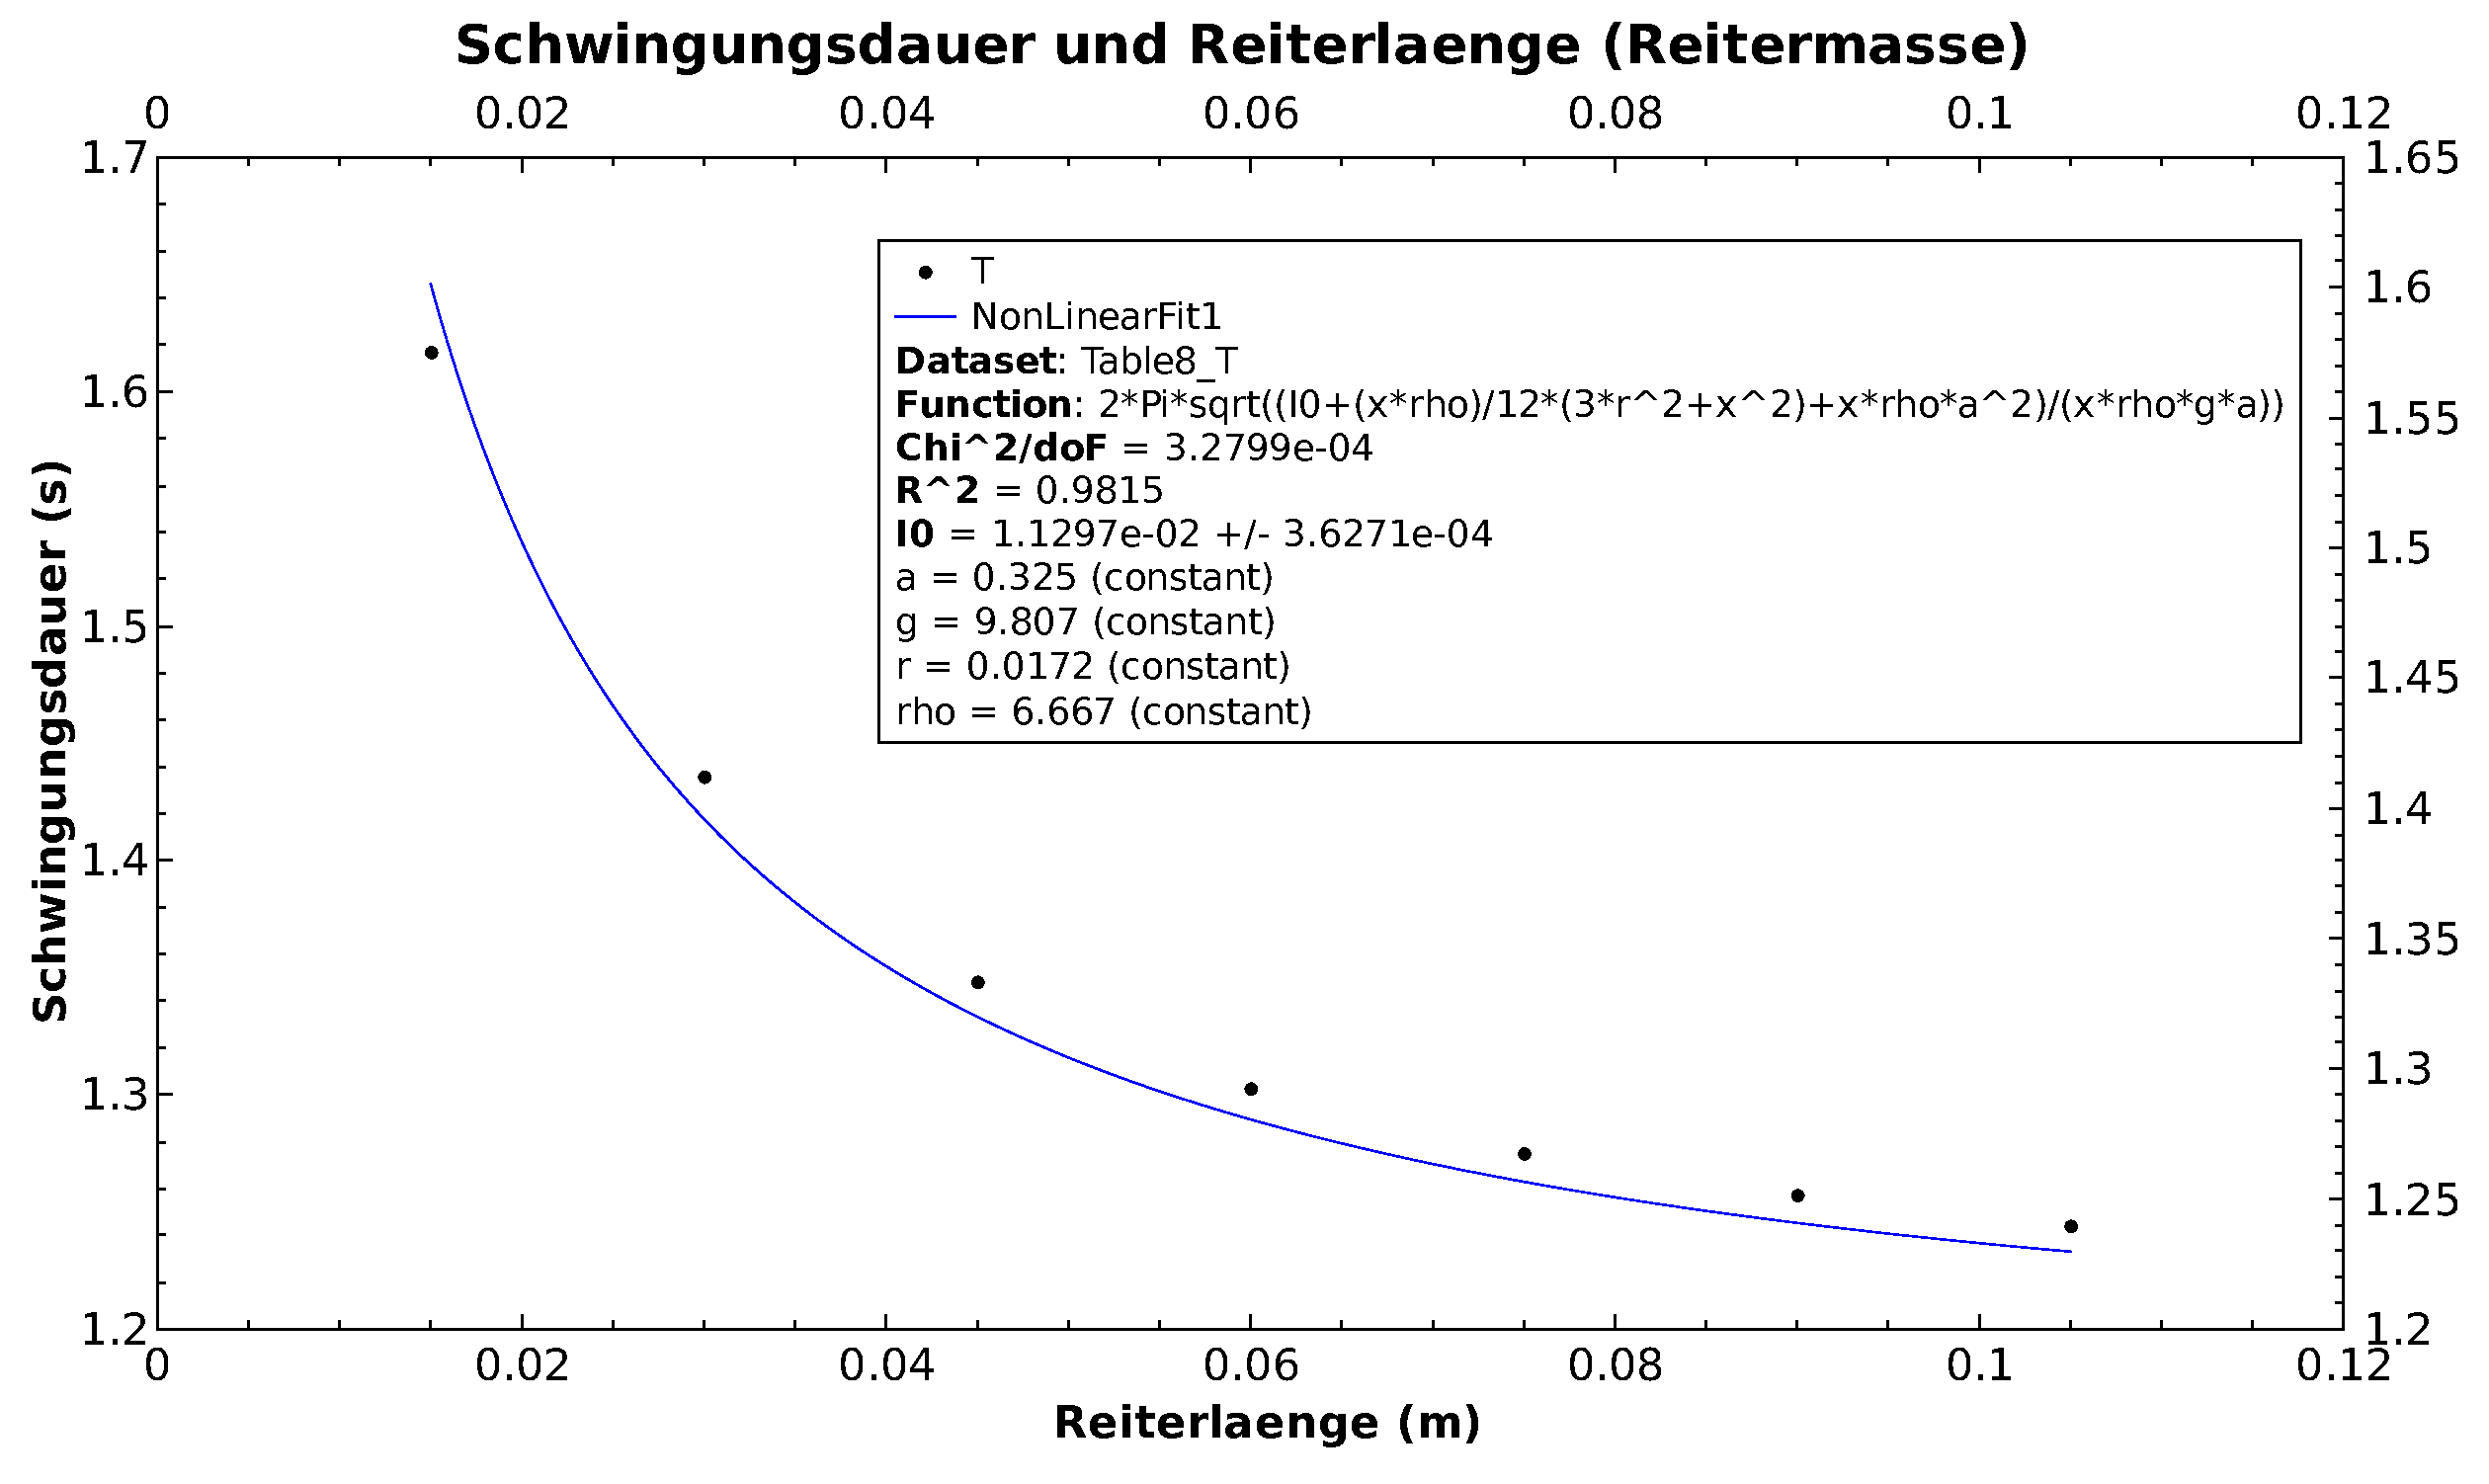
\includegraphics[width=\textwidth]{images/312b.pdf}
    \caption{%
        Schwingungsdauer in Abh\"angigkeit der Reitermasse, gefitted \"uber Tr\"agheitsmoment
    }
    \label{fig:312b}
\end{figure}

\clearpage
Man  kann  in  Abbildung  \ref{fig:312b}  erkennen, dass  nach  wie  vor  eine
Abweichung zwischen Fit und Messwerten besteht, allerdings scheint die Tendenz
der Differenz eher konstant und nicht zunehmend zu sein. Deshalb habe ich noch
einen  zus\"atzlichen  Fit  erstellt,  in dem  der  unterste  Messpunkt  nicht
ber\"ucksichtigt wird, was zum Fit in Abbildung \ref{fig:312c} f\"uhrt.

Dies ergibt
$I_0  = \SI[separate-uncertainty = true]{12.311 \pm 0.092950}{\gram\meter\squared}$.
Interessanterweise  ist die  Unsicherheit  hier merklich  kleiner, obwohl  ein
Messpunkt weniger verwendet wurde.

\begin{figure}[h!]
    \centering
    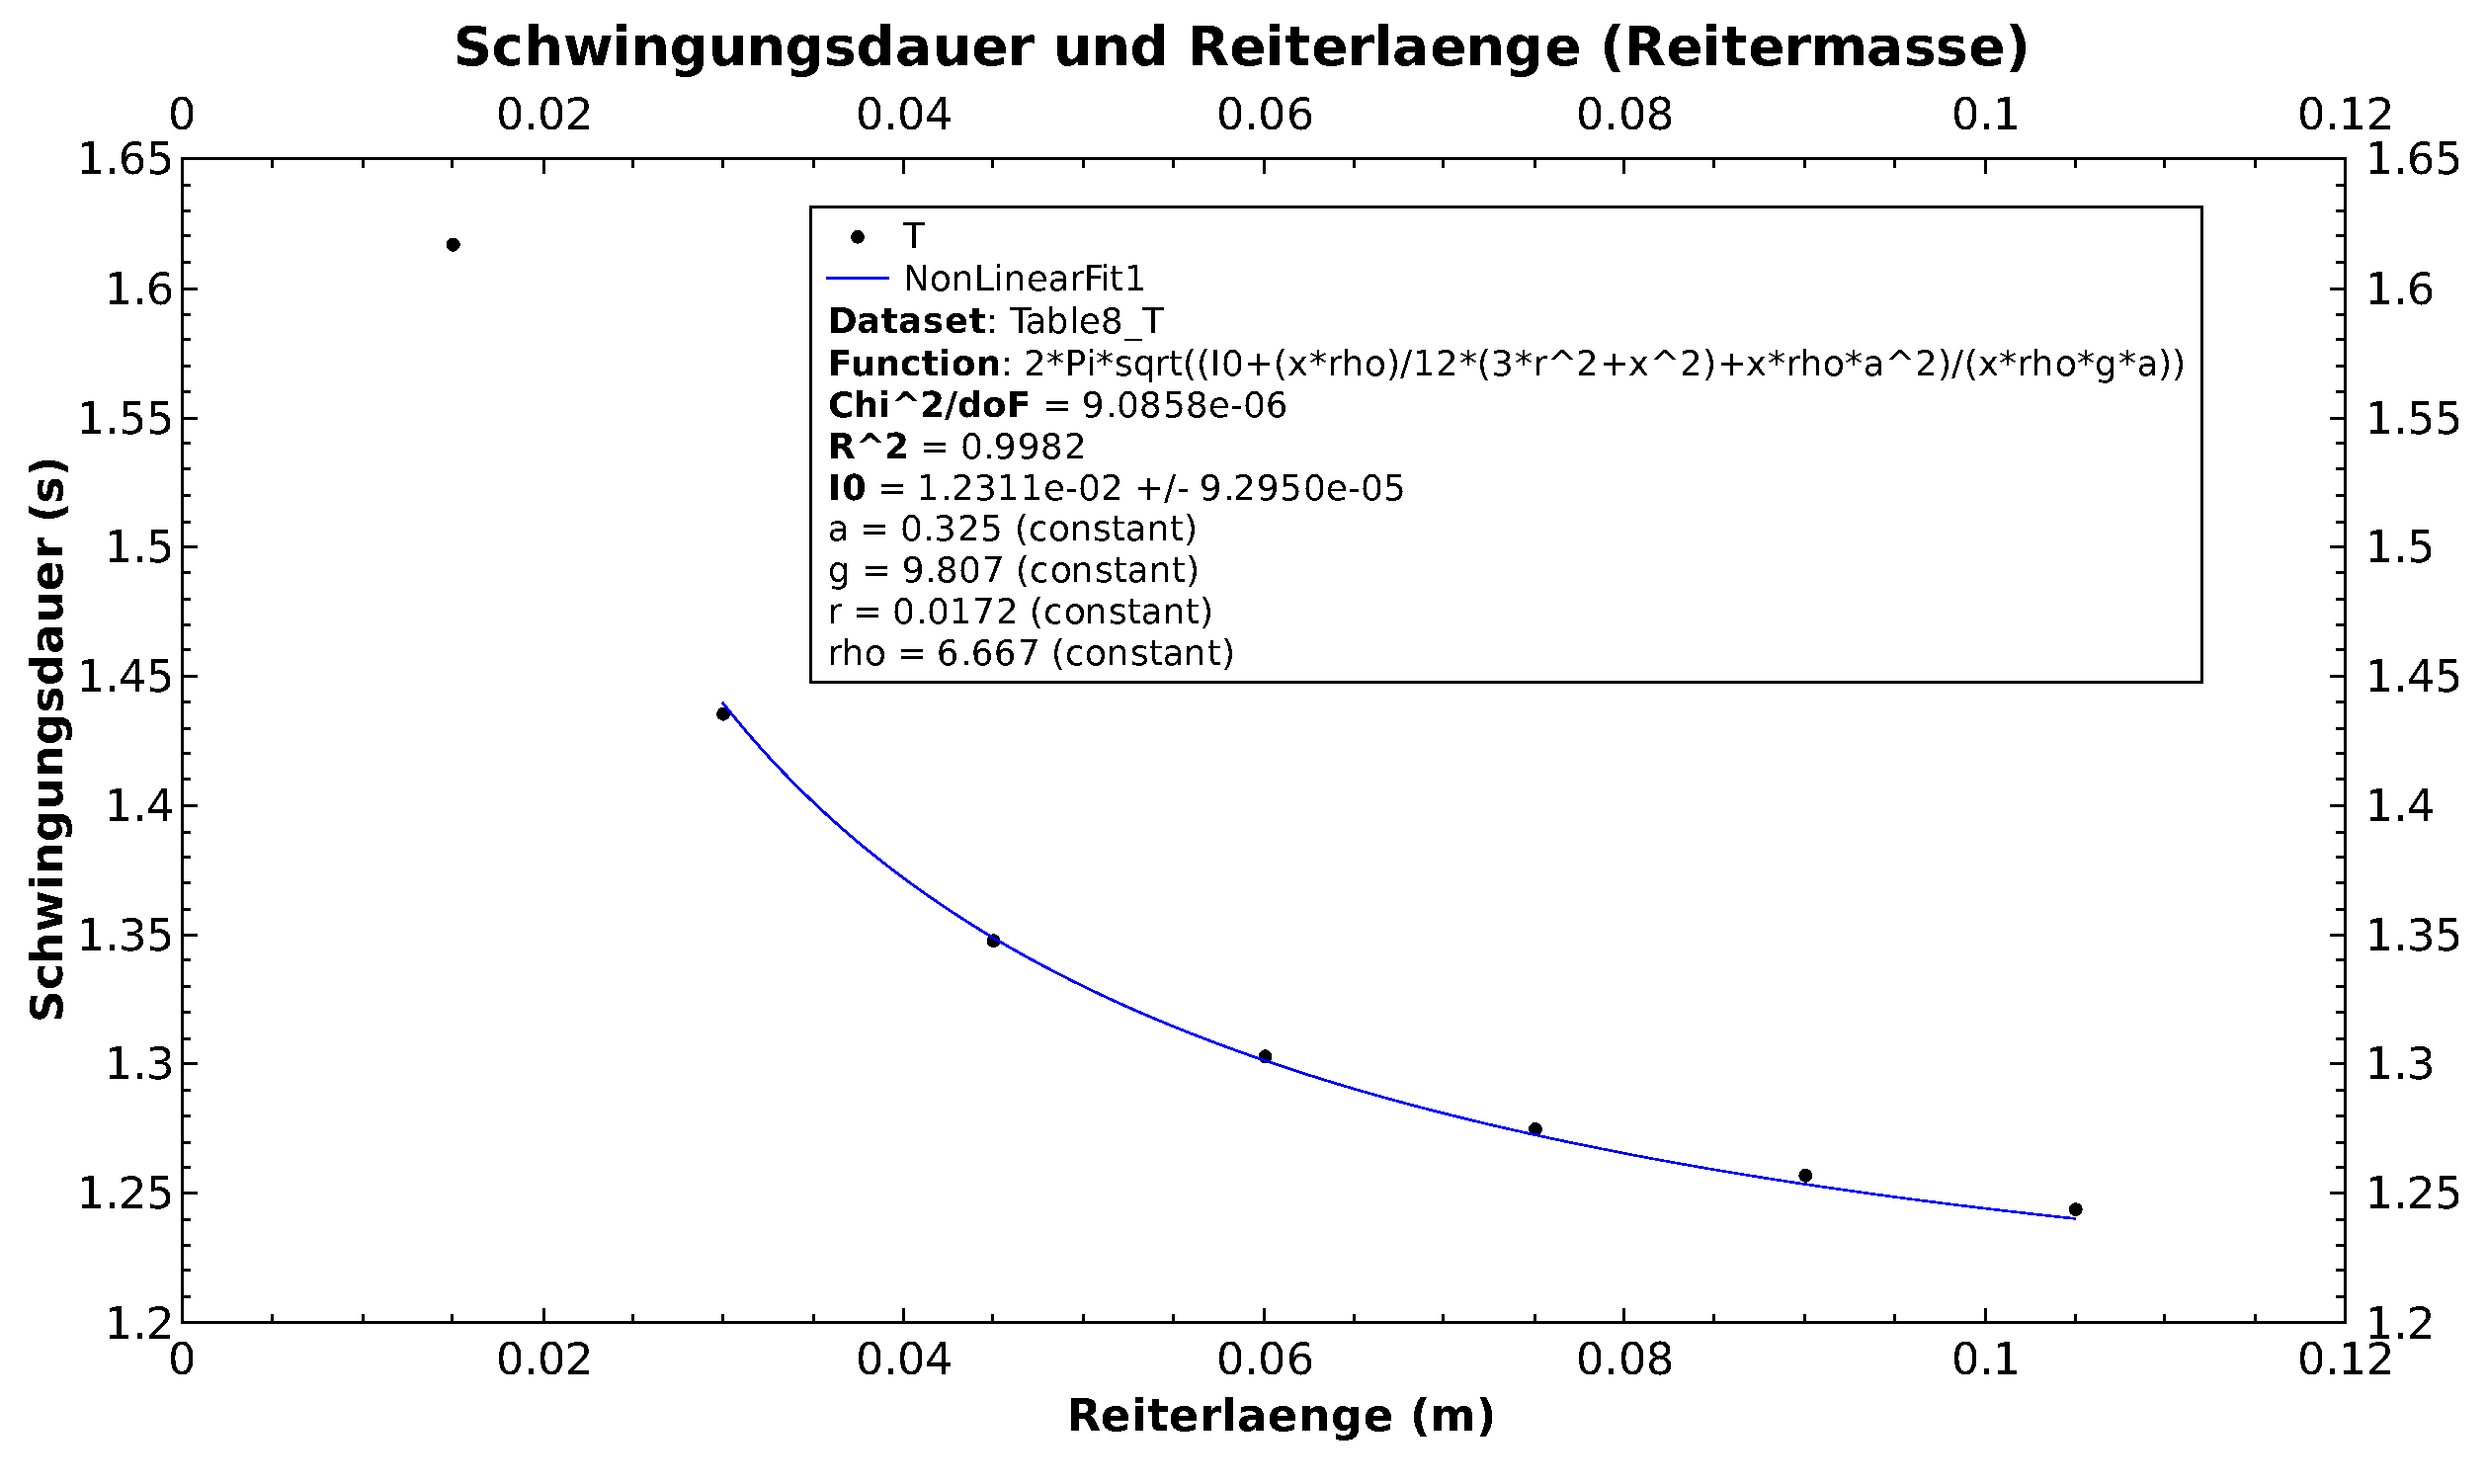
\includegraphics[width=\textwidth]{images/312c.pdf}
    \caption{%
        Schwingungsdauer in Abh\"angigkeit der Reitermasse, gefitted \"uber Tr\"agheitsmoment, unterster Messpunkt nicht ber\"ucksichtigt
    }
    \label{fig:312c}
\end{figure}

% ---------------------------------------------------------------------------- %
\clearpage
\subsection{Versuch 3.1.3 -- Periode in Abh\"angigkeit der Amplitude}
\label{subsec:periodeAmplitude}
% ---------------------------------------------------------------------------- %

Es wurde die gemessene Periode in Abh\"angigkeit der Amplitude mittels folgender
Formel gefittet:
\begin{equation}
    T = T_0 \cdot
        \left(
            1 +
            \left( \frac{1}{2} \right)^2 \cdot sin^2 \left( \frac{\hat{\varphi}}{2} \right)
            \left( \frac{1 \cdot 3}{2 \cdot 4} \right)^2 \cdot sin^4 \left( \frac{\hat{\varphi}}{2} \right)
            \left( \frac{1 \cdot 3 \cdot 5}{2 \cdot 4 \cdot 6} \right)^2 \cdot sin^6 \left( \frac{\hat{\varphi}}{2} \right)
            + ...
        \right)
\end{equation}

Zur Bestimmung der Anzahl n\"otigen Terme findet man im Anhang zu Versuch W4 folgendes
Diagramm:
\begin{figure}[h!]
    \centering
    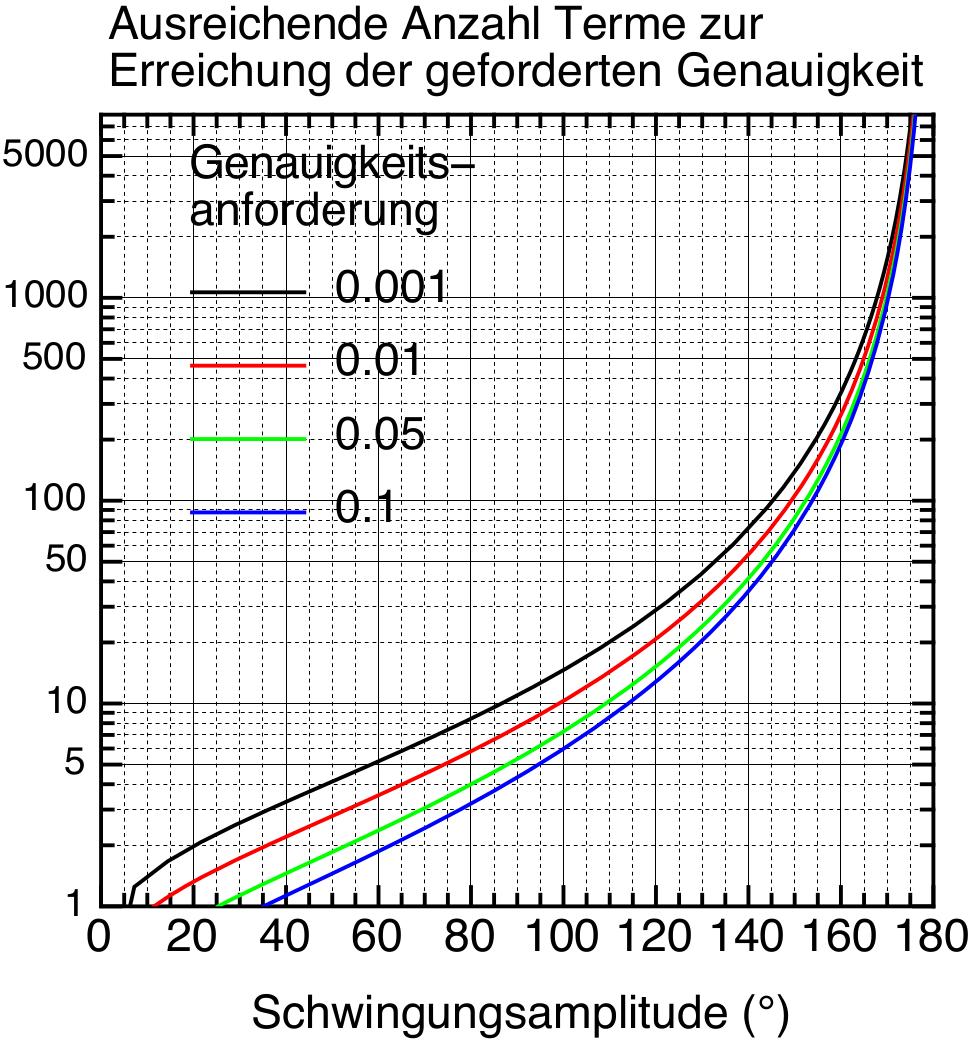
\includegraphics[width=.67\textwidth]{images/w4terme.png}
    \label{fig:w4terme}
    \caption{%
        Anzahl n\"otiger Terme in Abh\"angigkeit der gew\"unschten Genauigkeit
        und der maximalen Auslenkung.
    }
\end{figure}

Wir legen uns auf eine gew\"unschte Genauigkeit von \num{0.1} fest. Da wir bis
zu einem Winkel  von \SI{120}{\degree} gemessen haben,  ergibt dies ungef\"ahr
12 Terme (blaue Kurve).

Da  QtiPlot bei  12  Summanden abst\"urzte,  wurde die  Funktion  nur bis  zur
18. Potenz des Sinus gefittet.

\begin{figure}[h!]
    \centering
    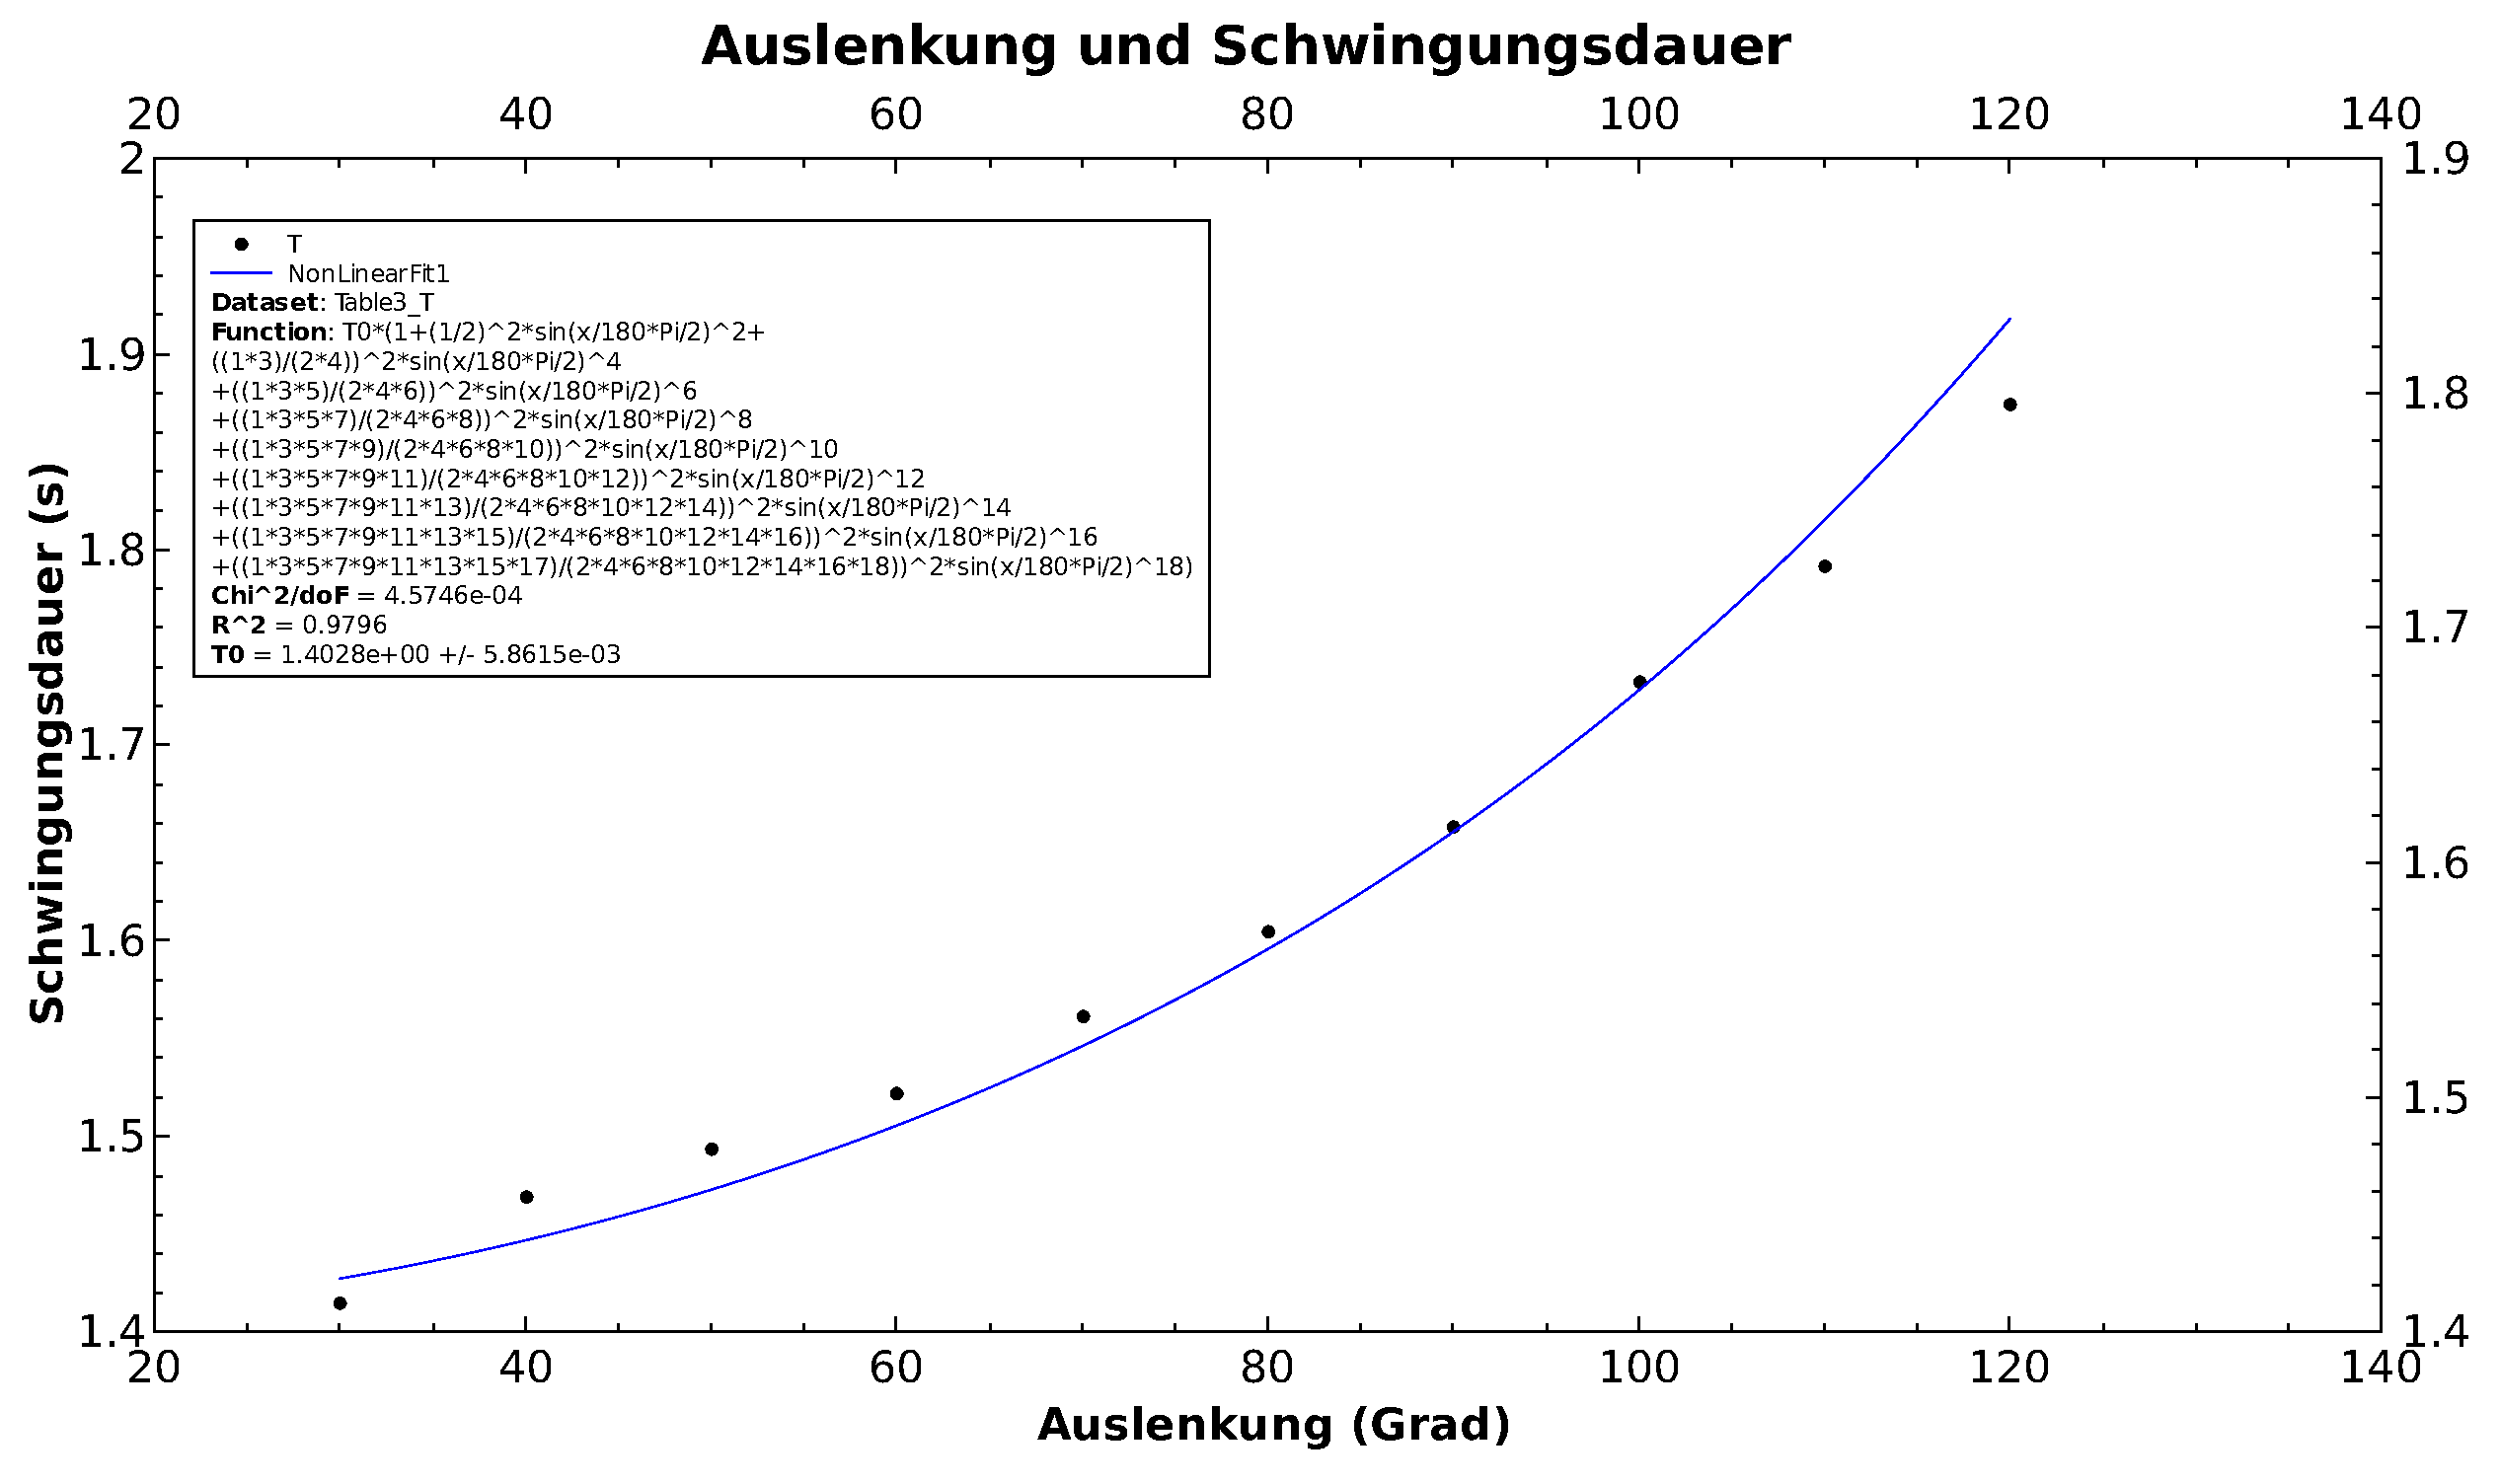
\includegraphics[width=\textwidth]{images/313.pdf}
    \label{fig:pendelKonfigs}
    \caption{%
        Schwingungsdauer in Abh\"angigkeit der Auslenkung
    }
\end{figure}

Da der  untereste Wert  nach einem  Ausreisser aussieht  und die  oberen Werte
aufgrund  von Reibungseffekten  vermutlich  nicht mehr  allzu pr\"azise  sind,
wurde noch ein zweiter Fit mit eingeschr\"anktem Bereich durchgef\"uhrt.

\begin{figure}[h!]
    \centering
    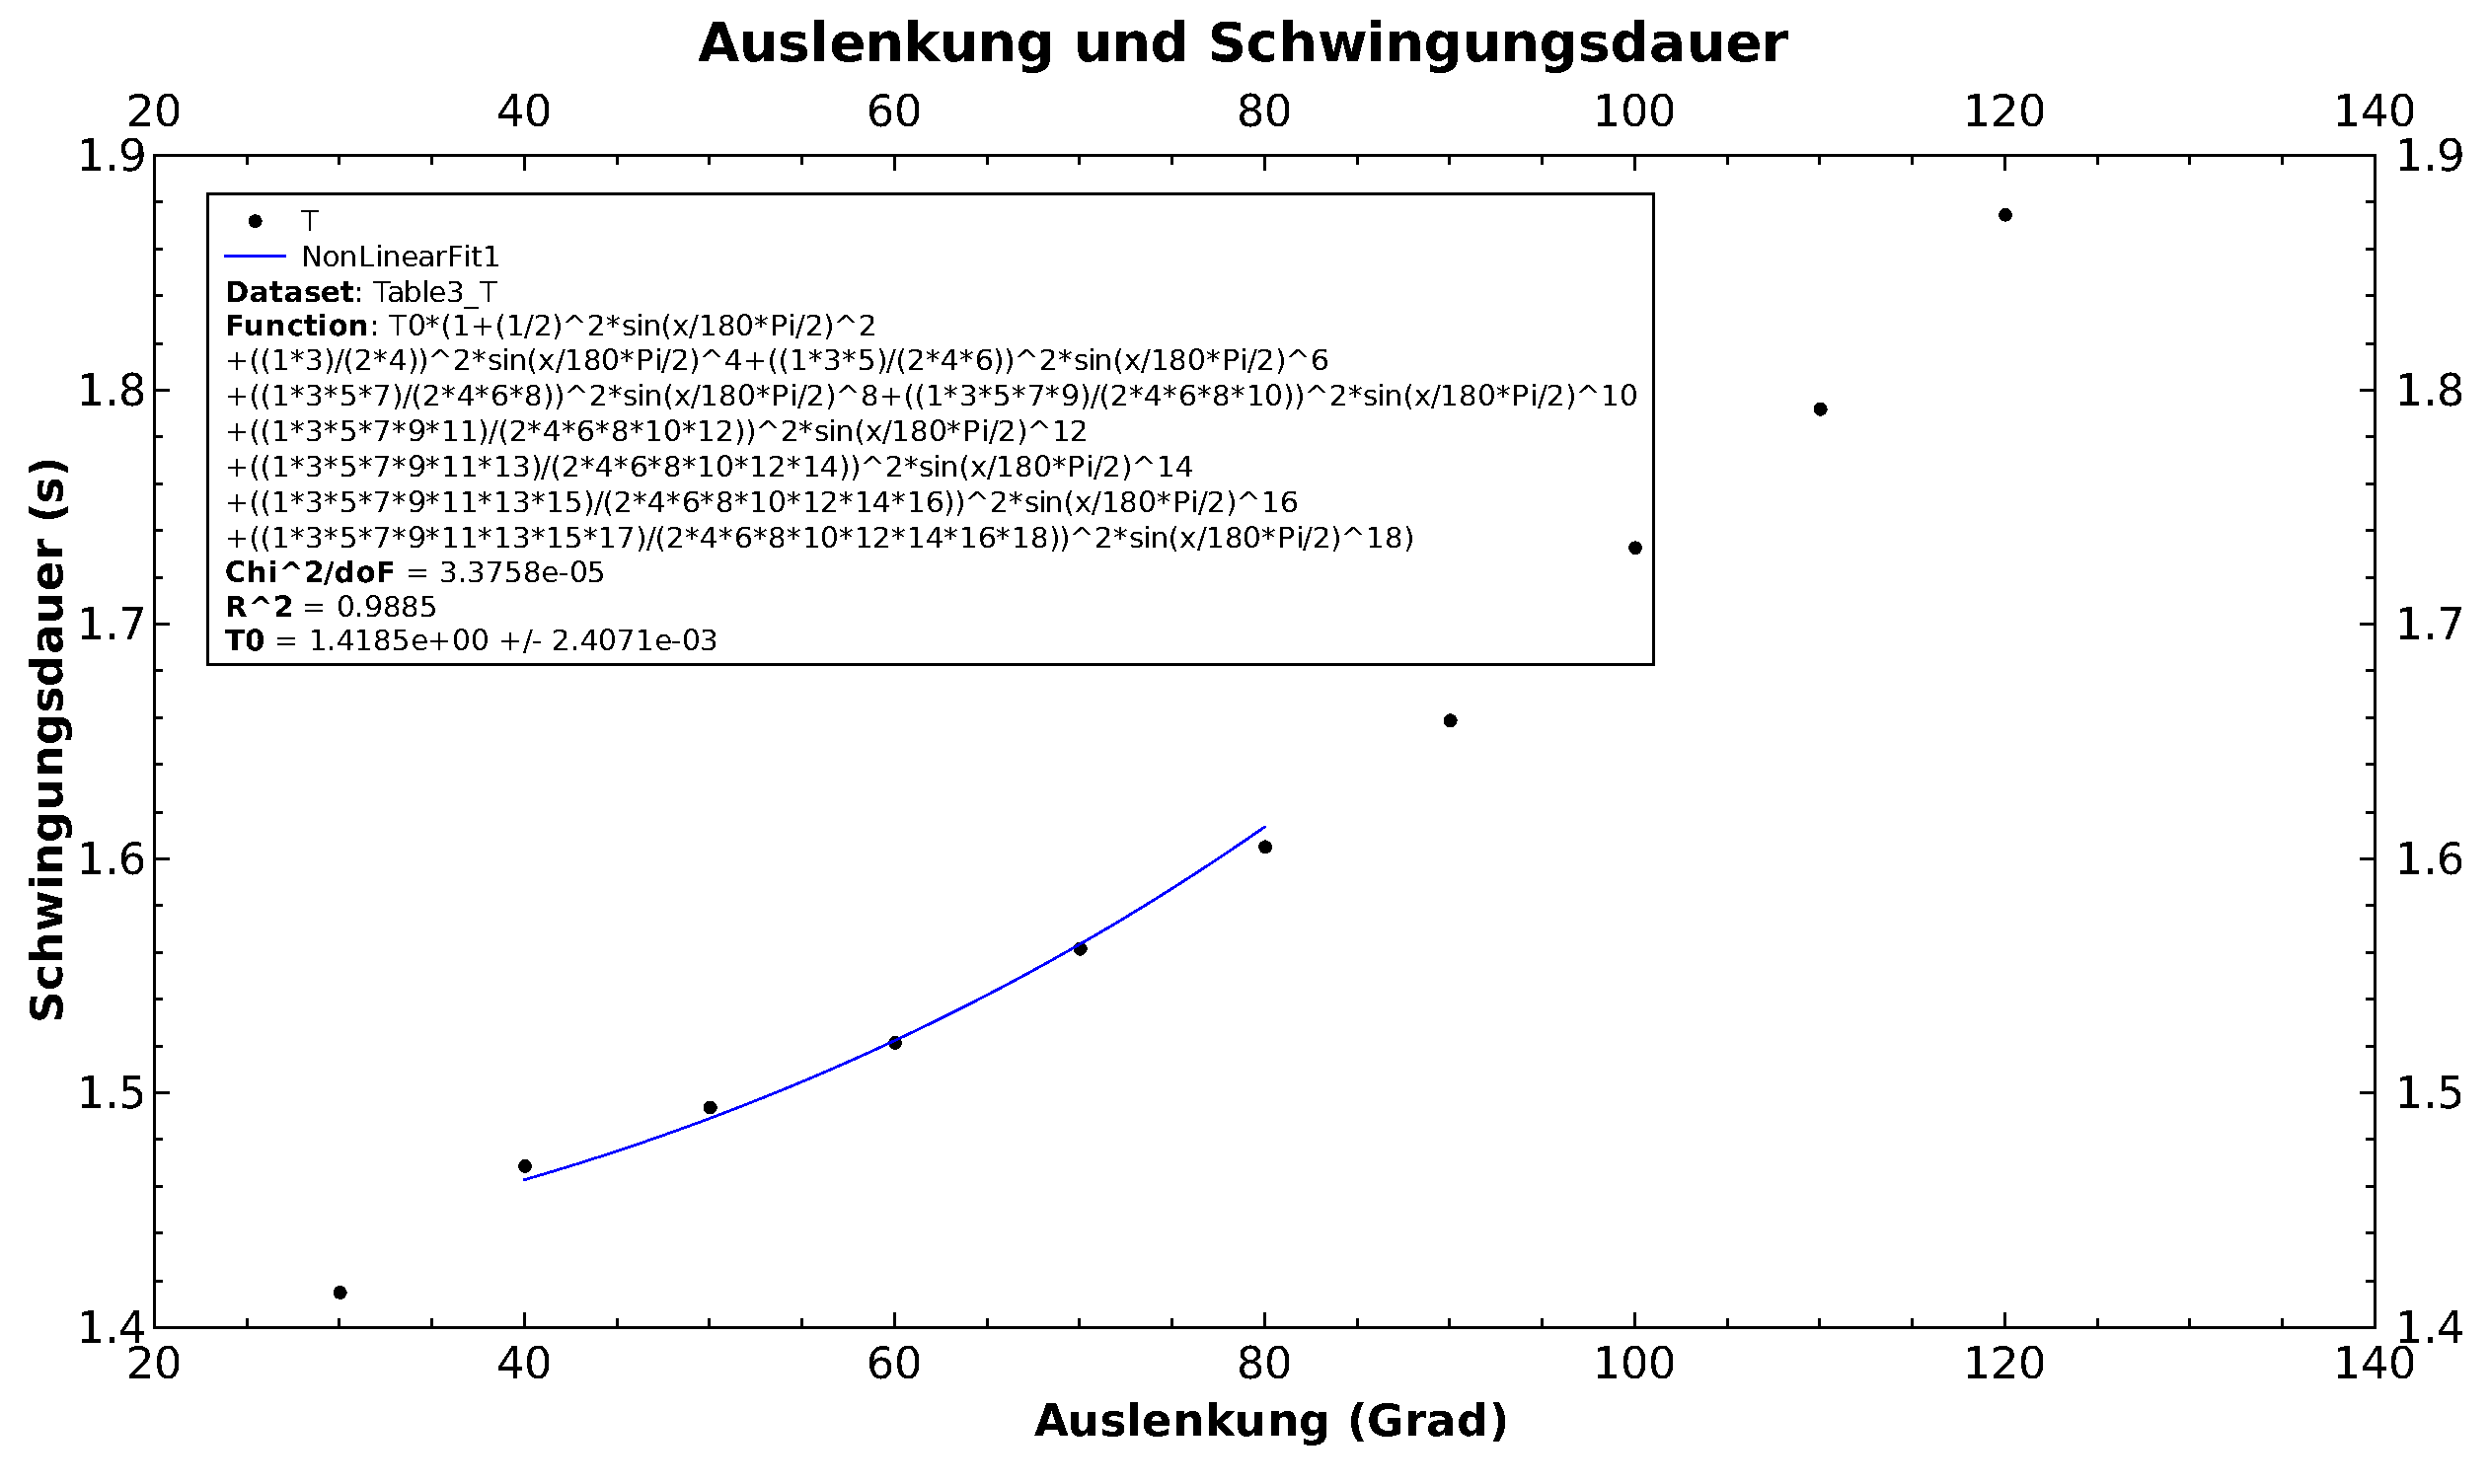
\includegraphics[width=\textwidth]{images/313b.pdf}
    \label{fig:pendelKonfigs}
    \caption{%
        Schwingungsdauer in Abh\"angigkeit der Auslenkung, eingeschr\"ankter Bereich.
    }
\end{figure}
$T_0  = \SI[separate-uncertainty = true]{1.4028 \pm 0.0058615}{\second}$.
$T_0  = \SI[separate-uncertainty = true]{1.4185 \pm 0.0024071}{\second}$.

% ---------------------------------------------------------------------------- %
\clearpage
\subsection{Versuch 3.3.1 -- Kombipendel Konfiguration 2}
\label{subsec:kombiKonfig2}
% ---------------------------------------------------------------------------- %


% ---------------------------------------------------------------------------- %
\subsubsection{Reiterposition variabel}
% ---------------------------------------------------------------------------- %

Hier wird folgende Formel zum Fitten verwendet:

\begin{equation}
    T = 2 \cdot \pi \cdot \sqrt{\frac{I}{p + q}}
\end{equation}

Die Federn und die Reitermasse wirken beide in die gleich Richtung r\"uckstellend,
daher das Plus-Zeichen im Nenner.

$I$ setzt sich  hier zusammen aus dem  oben bestimmten Massentr\"agheitsmoment
$I_0$ der Apparatur, aus  dem Massentr\"agheitsmoment $I_{Reiter}$ des Reiters
(approximiert  als   Punktmasse,  da  hier  der   Reiter  mit  \SI{200}{\gram}
verwendet  wurde)  und  dem  Anteil  $I_{Federn}$  der  Federn. Gefittet  wird
dann  \"uber die  Federkonstante $k$  im  Parameter $p  = 2kr^2$,  wobei $r  =
\SI{80.2}{\milli\meter}$ der Angriffsradius der  Federn an der Seilscheibe ist
(plus der Radius des Seils).

Es gilt also:
\begin{itemize}
    \item
        $I_0 = $
    \item
        $I_{Reiter} = \SI{200}{\gram} \cdot a^2$
    \item
        $I_{Federn} = \frac{1}{3} \cdot m_{Federn} \cdot \SI{80.2}{\milli\meter}^2$
    \item
        $p = 2 \cdot k \cdot \SI{80.2}{\milli\meter}^2$
    \item
        $q = m \cdot g \cdot a$ ($a$: Reiterposition)
\end{itemize}

Die   Masse   der   Federn    ist   \SI{155.5}{\gram}   f\"ur   beide   Federn
kombiniert. F\"ur das Massentr\"agheitsmoment $I_0$ verwenden wir den Wert von
\SI{12.311}{\gram\meter\squared} aus dem eingeschr\"ankten Fit.

Somit erh\"ahlt man als Formel f\"ur T:

\begin{equation}
    T = 2 \cdot \pi \cdot \sqrt{\frac{\SI{12.311}{\gram\meter\squared} + \SI{155.5}{\gram} \cdot (\SI{80.2}{\milli\meter})^2 + \SI{200}{\gram} \cdot a^2}{2 \cdot k \cdot (\SI{80.2}{\milli\meter})^2 + \SI{200}{\gram} \cdot
    \SI{9.807}{\meter\per\second\squared} \cdot a}}
\end{equation}

$a$ entspricht der x-Achse, gefittet wird \"uber $k$.

\begin{figure}[h!]
    \centering
    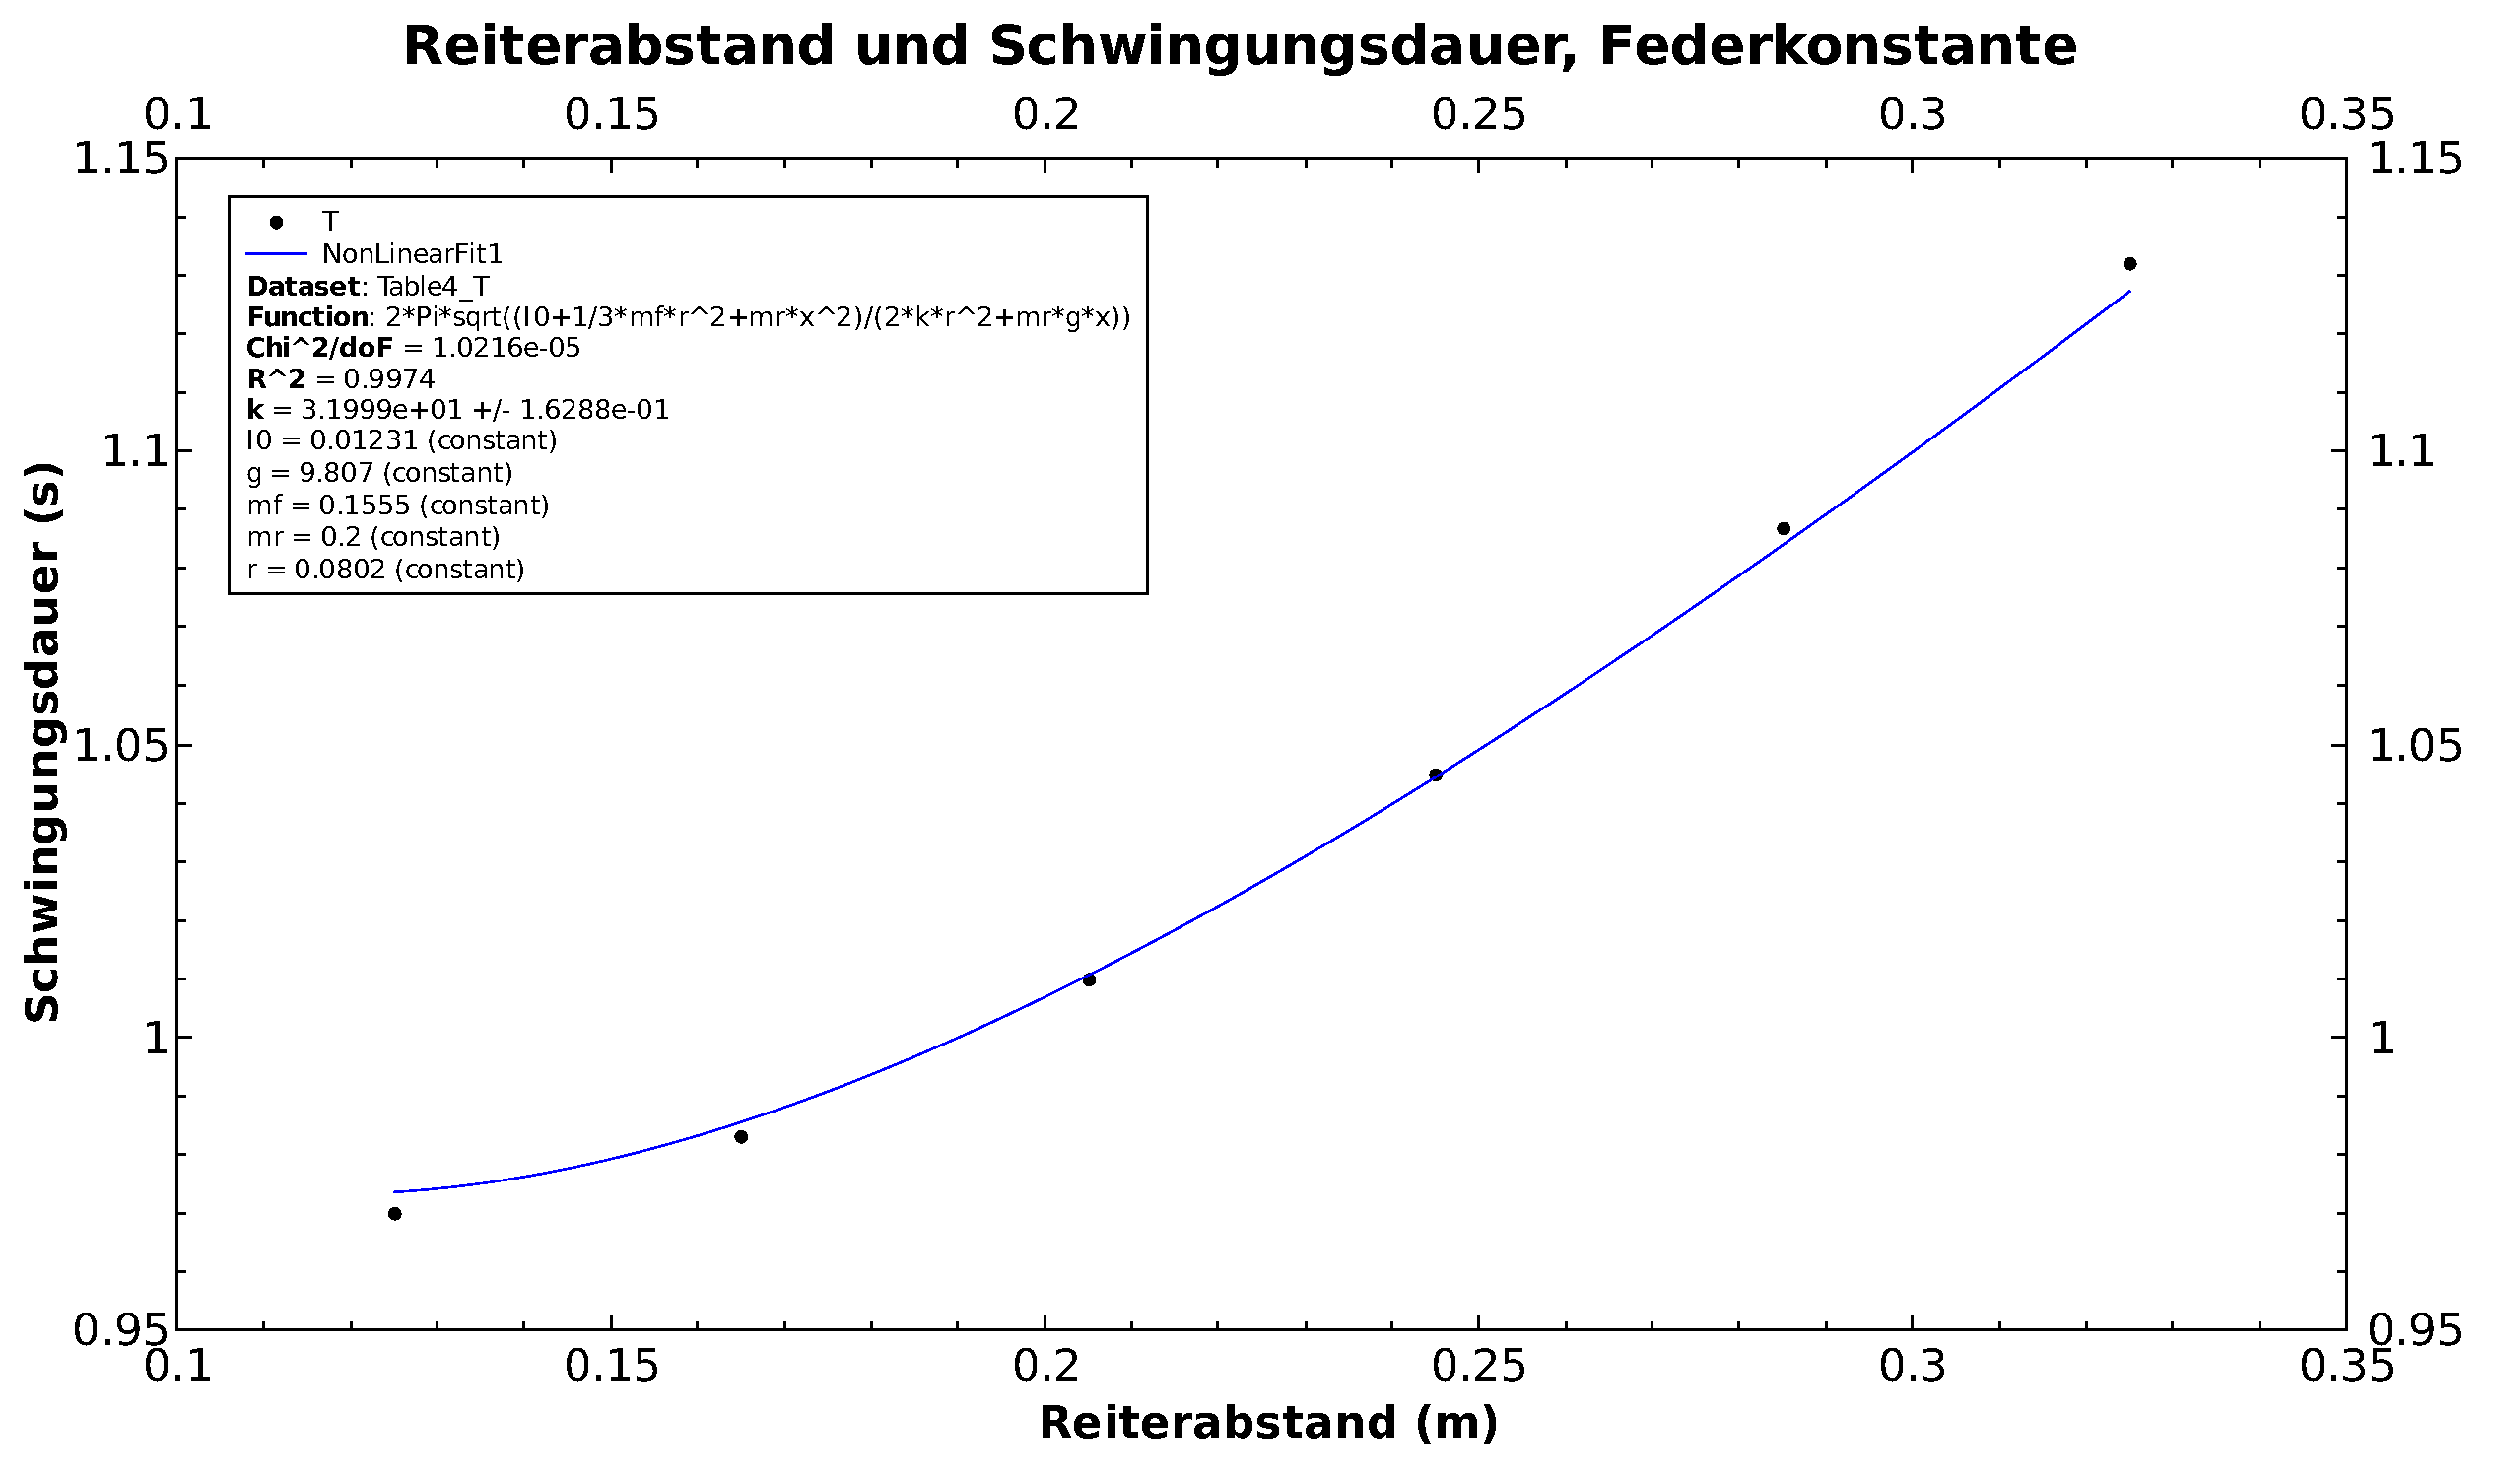
\includegraphics[width=\textwidth]{images/331a.pdf}
    \caption{%
        Schwingungsdauer in Abh\"angigkeit der Reiterposition beim Kombipendel, gefittet f\"ur Federkonstante $k$
    }
    \label{fig:331a}
\end{figure}

Aus dem  in Abbildung  \ref{fig:331a} dargestellten Fit  ergibt sich  ein Wert
f\"ur die  Federkonstante von  $k = \SI[separate-uncertainty  = true]{31.999
\pm  0.16288}{\newton\per\meter}$,  was  ziemlich   nahe  beim  Wert  aus  der
Versuchsanleitung von \SI{32}{\newton\per\meter} ist.


% ---------------------------------------------------------------------------- %
\clearpage
\subsubsection{Auslenkung variabel}
\label{subsubsec:kombiP:auslvar}
% ---------------------------------------------------------------------------- %

Bei dieser Messung stimmt offensichtlich etwas nicht so ganz, allerdings bin ich
mir nicht sicher, wo der Fehler genau liegt.


\begin{figure}[h!]
    \centering
    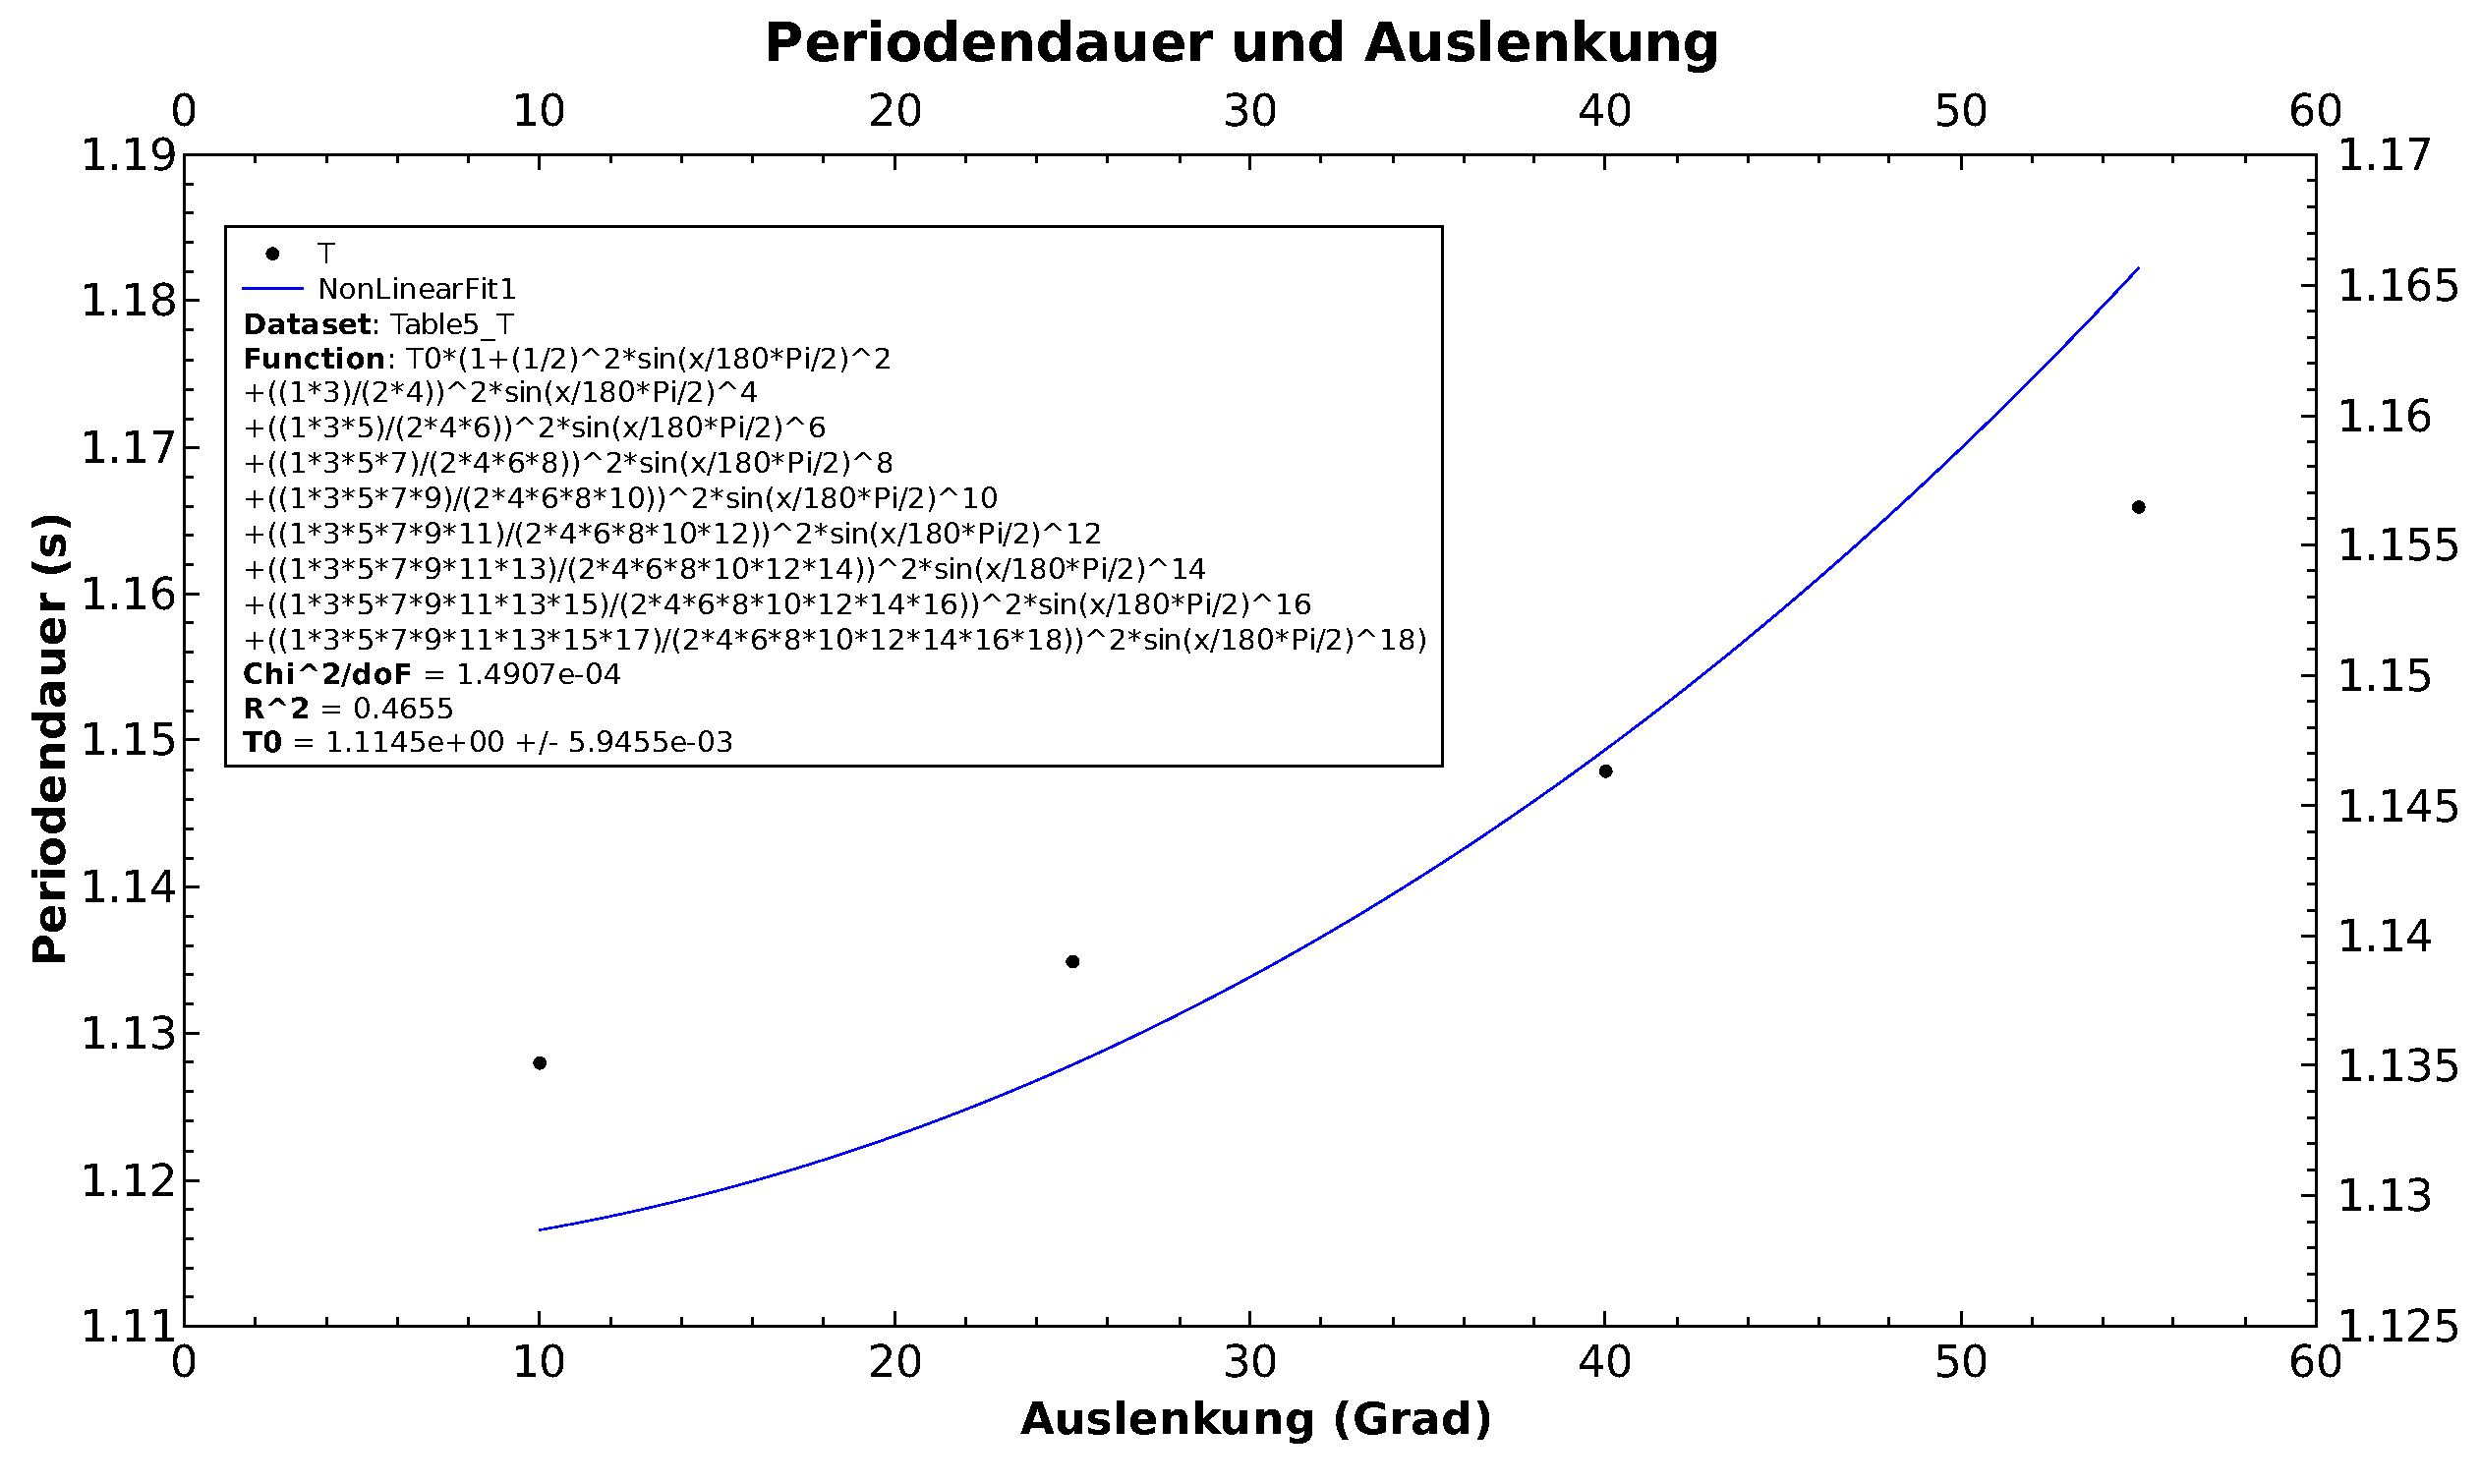
\includegraphics[width=\textwidth]{images/331b.pdf}
    \caption{%
        Schwingungsdauer in Abh\"angigkeit der Auslenkung beim Kombipendel
    }
    \label{fig:331b}
\end{figure}

Der   Fit   aus   Abbildung   \ref{fig:331b}  ergibt   einen   Wert   $T_0   =
\SI[separate-uncertainty  = true]{1.4028  \pm  0.0058615}{\second}$, was  zwar
einigermassen plausibel erscheint (verglichen  mit den Messwerten), jedoch ist
der Kurvenverlauf nicht wirklich passend zu den Messwerten. Allenfalls w\"aren
hier noch mehr Messungen durchzuf\"uhren.

F\"ur   die   Anzahl   Terme   wurden   hier   die   gleichen   \"Uberlegungen
gemacht  wie  bereits  in Abschnitt  \ref{subsec:periodeAmplitude}  auf  Seite
\pageref{subsec:periodeAmplitude} dokumentiert.




% ---------------------------------------------------------------------------- %
\clearpage
\subsection{Versuch 3.3.2 -- Kombipendel Konfiguration 3}
\label{subsec:kombiKonfig3}
% ---------------------------------------------------------------------------- %

Der  kritische  Abstand  $a_{krit}$  wurde  durch  Probieren  auf  einen  Wert
zwischen  $\SI{195}{\milli\meter}$ und  $\SI{205}{\milli\meter}$ bestimmt. Die
Versuchsreihe  wurde  daher mit  Werten  von  $a \leq  \SI{195}{\milli\meter}$
durchgef\"uhrt. Da Reitermasse und Federkraft sich hier entgegenwirken, ist im
Nenner zwischen $p$ und $q$ ein Minuszeichen zu finden.

\begin{figure}[h!]
    \centering
    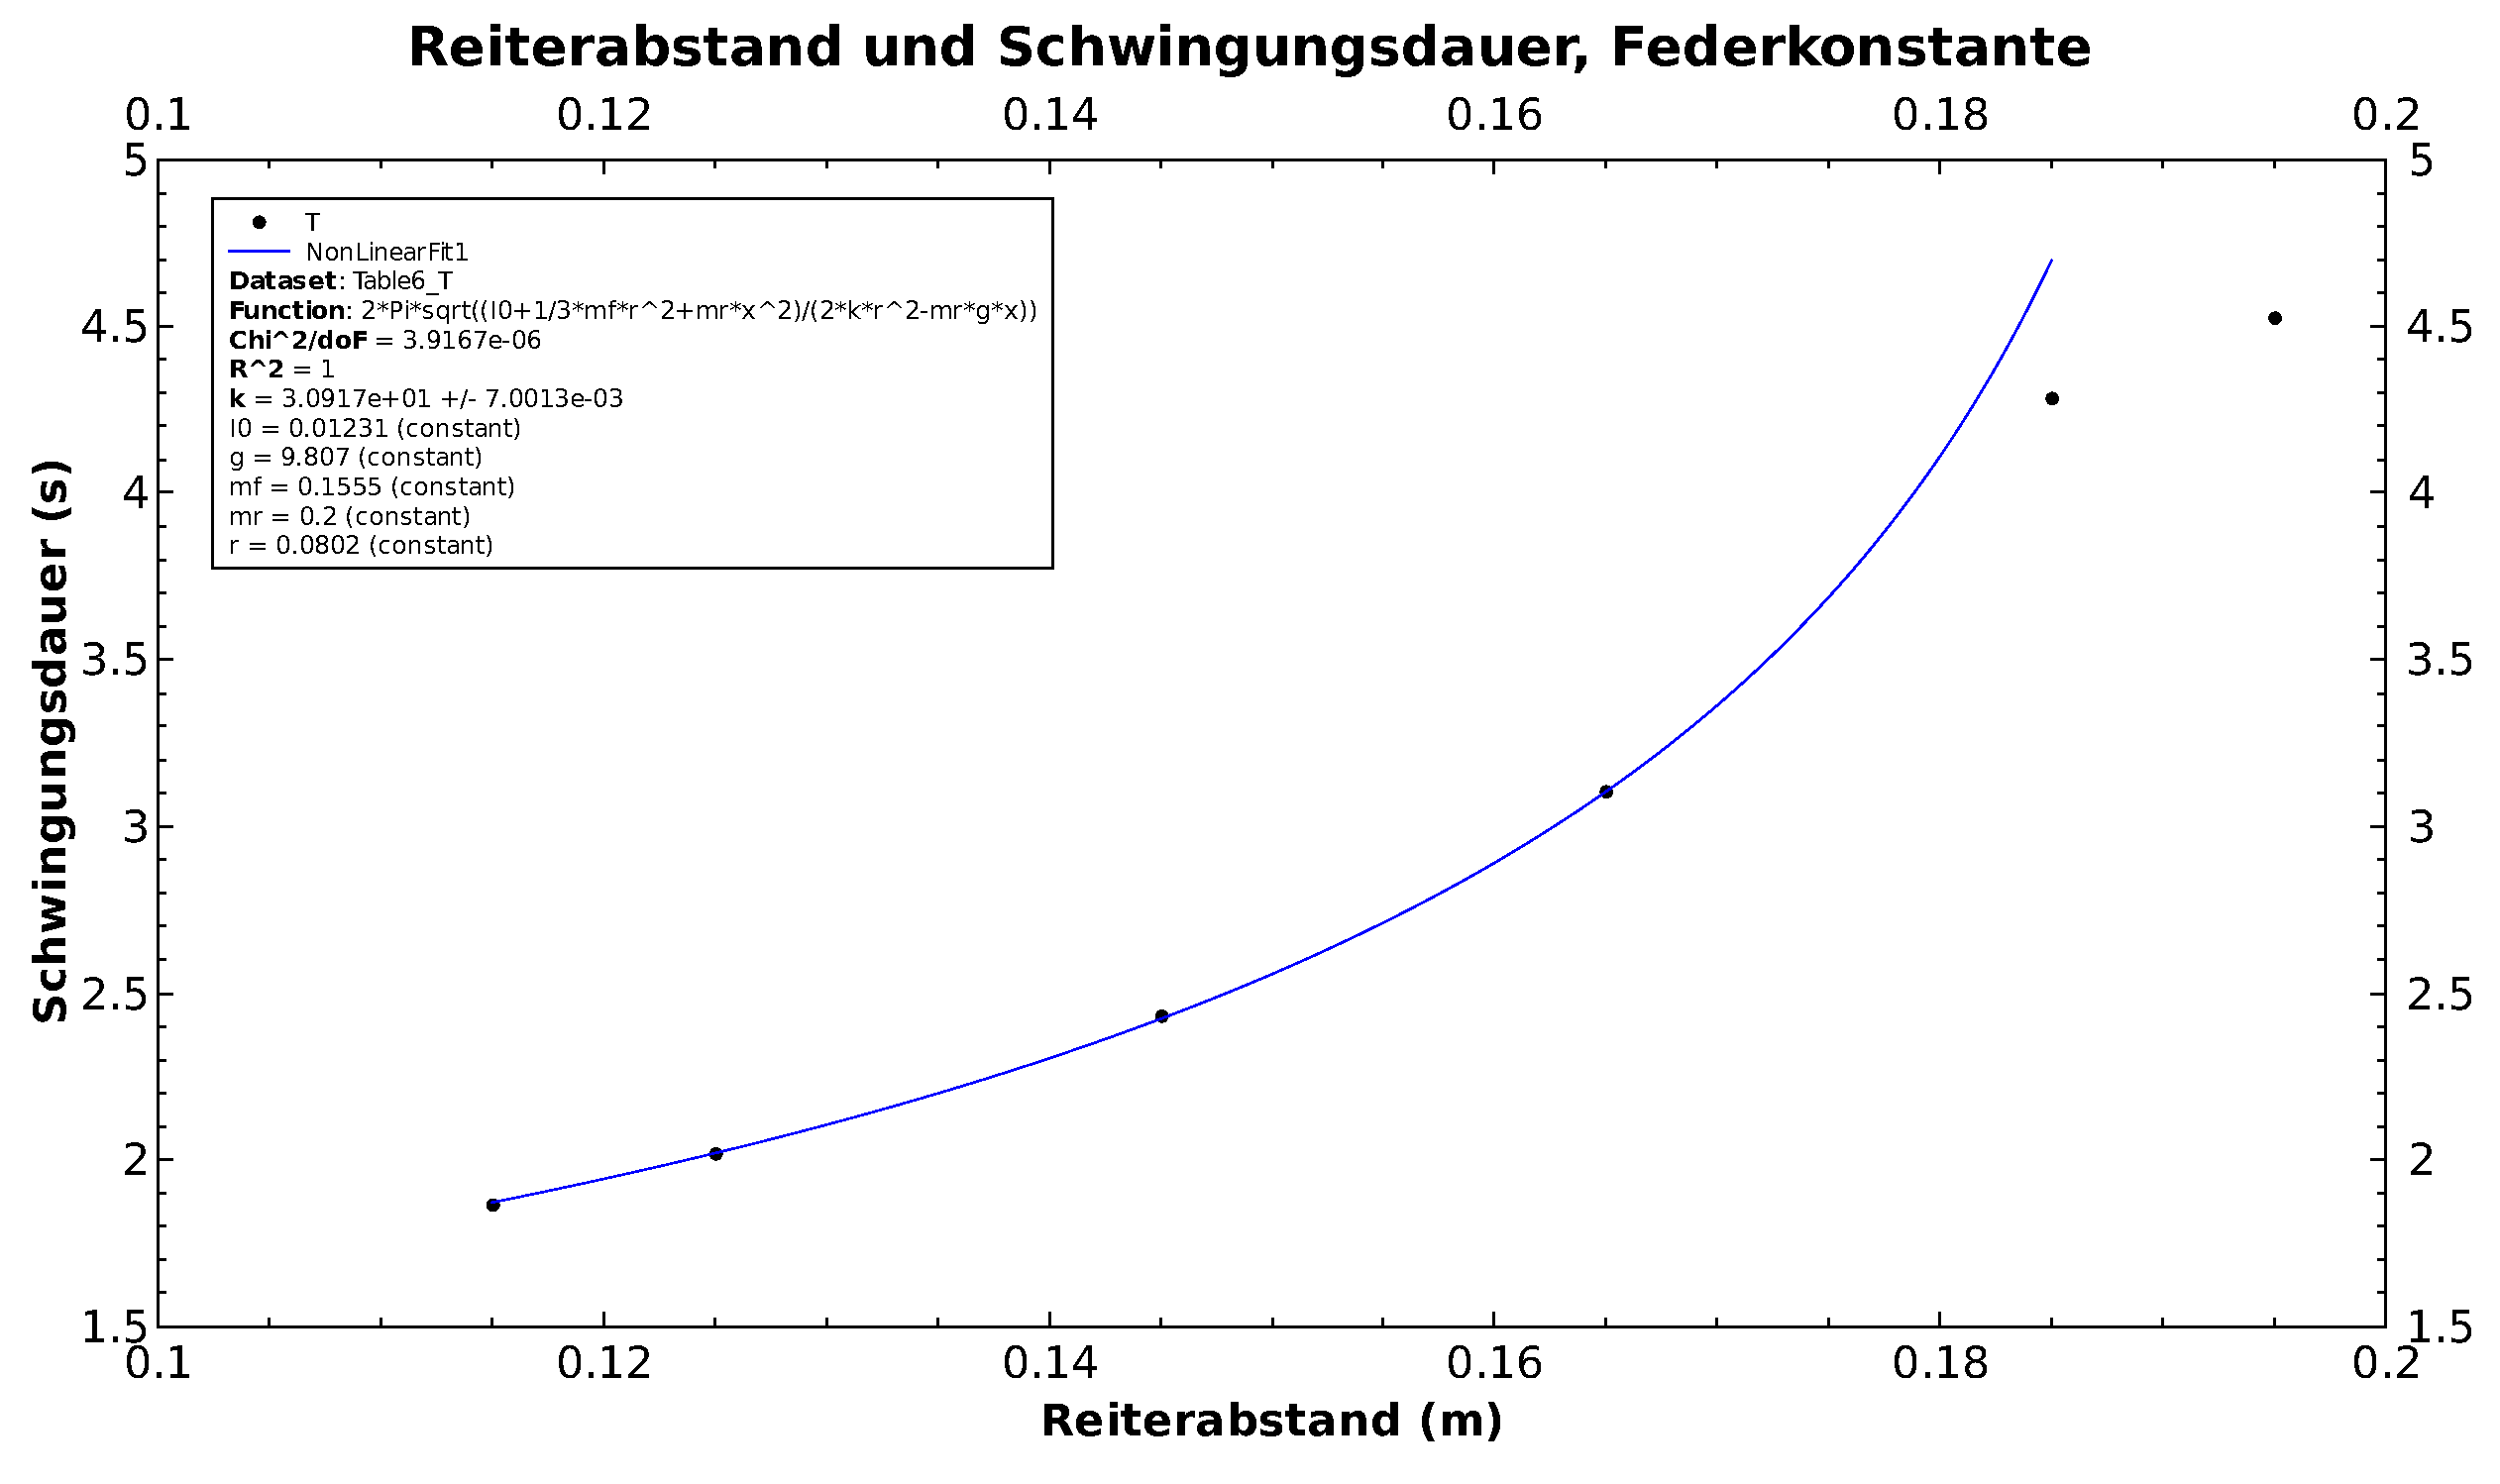
\includegraphics[width=\textwidth]{images/332.pdf}
    \label{fig:pendelKonfigs}
    \caption{%
        Schwingungsdauer in Abh\"angigkeit der Reiterposition beim invertierten Kombipendel unterhalb des kritischen Abstandes. Letzter Messpunkt wurde als Ausreisser behandelt und im Fit nicht ber\"ucksichtigt.
    }
\end{figure}

Die verwendeten Parameter sind
\begin{itemize}
    \item
        $I_0  = \SI[separate-uncertainty = true]{12.311}{\gram\meter\squared}$.
    \item
        $g = \SI{9.807}{\meter\per\second\squared}$
    \item
        $m_{Federn} = \SI{155.5}{\gram}$
    \item
        $m_{Reiter} = \SI{200}{\gram}$
    \item
        $r = \SI{80.2}{\milli\meter}$
\end{itemize}

Gefittet wurde  wiederum f\"ur  die Federkonstante,  was einen  Wert von:

$k = \SI[separate-uncertainty  =  true]{30.917 \pm  0.0070013}{\newton\per\meter}$,

was auch ziemlich nahe beim Wert aus der Versuchsanleitung liegt.

% ---------------------------------------------------------------------------- %
\clearpage
\subsection{Versuch 3.3.3 -- Ruhelagen}
\label{subsec:ruhelagen}
% ---------------------------------------------------------------------------- %


% ---------------------------------------------------------------------------- %
\subsubsection{Reiterposition}
\label{subsubsec:reiterpos}
% ---------------------------------------------------------------------------- %


Auch  mit dem  invertierten Pendel  und dem  Reiter ausserhalb  des kritischen
Abstandes kann  wiederum die  Federkonstante $k$  bestimmt werden. Allderdings
muss hier eine andere Formel verwendet werden:

\begin{equation}
    \frac{\varphi_0}{sin(\varphi_0)} = \frac{a}{a_G} = \frac{q}{p} = \frac{m_{Reiter} \cdot g \cdot a}{2 \cdot k \cdot r^2}
\end{equation}

Wobei $r =  \SI{80.2}{\milli\meter}$, $m_{Reiter} = \SI{200}{\gram}$  und $g =
\SI{9.807}{\meter\per\second\squared}$. $a$  entspricht der  x-Achse, gefittet
wurde \"uber $k$.

\begin{figure}[h!]
    \centering
    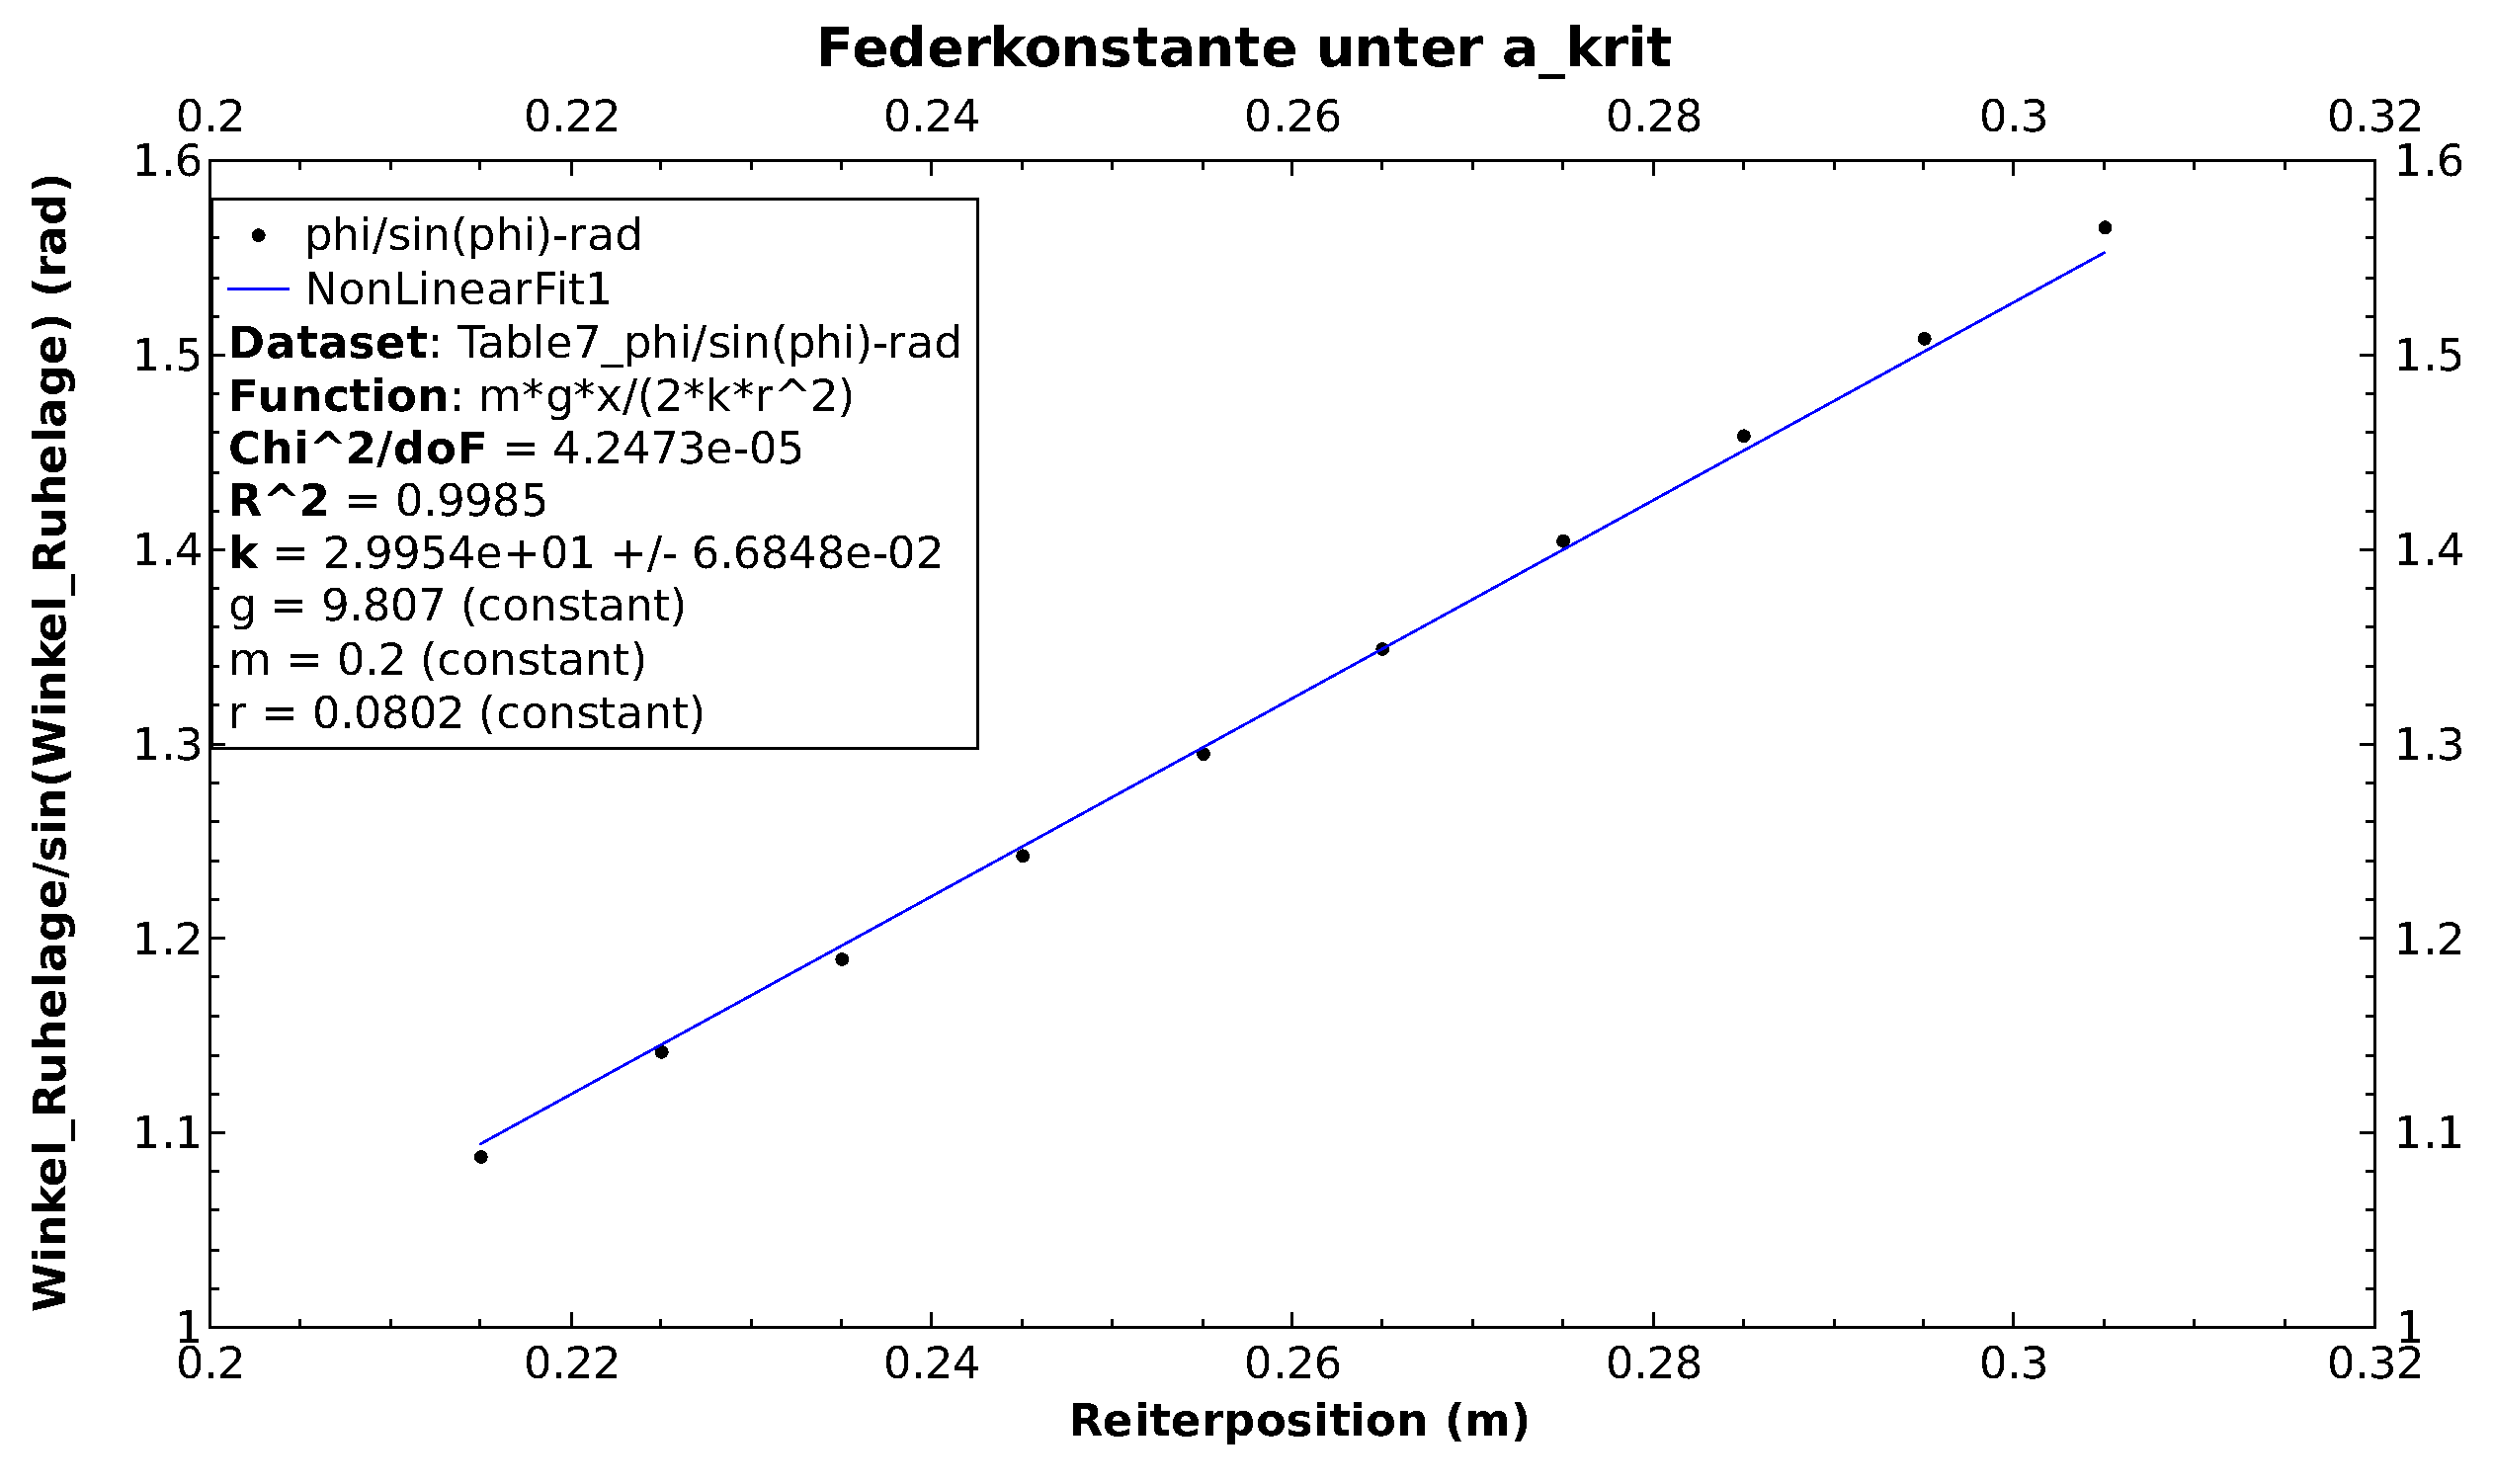
\includegraphics[width=\textwidth]{images/333a.pdf}
    \caption{%
        Bestimmung des Parameters $k$ via Ruhelage, $a>a_{krit}$
    }
    \label{fig:333a}
\end{figure}

Aus dem Fit in Abbildung \ref{fig:333a} erh\"alt man also
$k = \SI[separate-uncertainty  =  true]{29.954 \pm  0.066848}{\newton\per\meter}$.
Auch dieses Ergebnis scheint mir recht zufriedenstellend.


% ---------------------------------------------------------------------------- %
\clearpage
\subsubsection{Schwingungsdauer}
\label{subsubsec:schwingungsdauer}
% ---------------------------------------------------------------------------- %

Zu  guter  letzt  sind  in  Abbildung  \ref{fig:333b}  die  Periodenzeiten  in
Ab\"angigkeit   der  Reiterposition   ausserhalb   des  kritischen   Abstandes
geplotted. Es wurde aber gem\"ass Versuchsanleitung kein Fit ausgef\"uhrt.

\begin{figure}[h!]
    \centering
    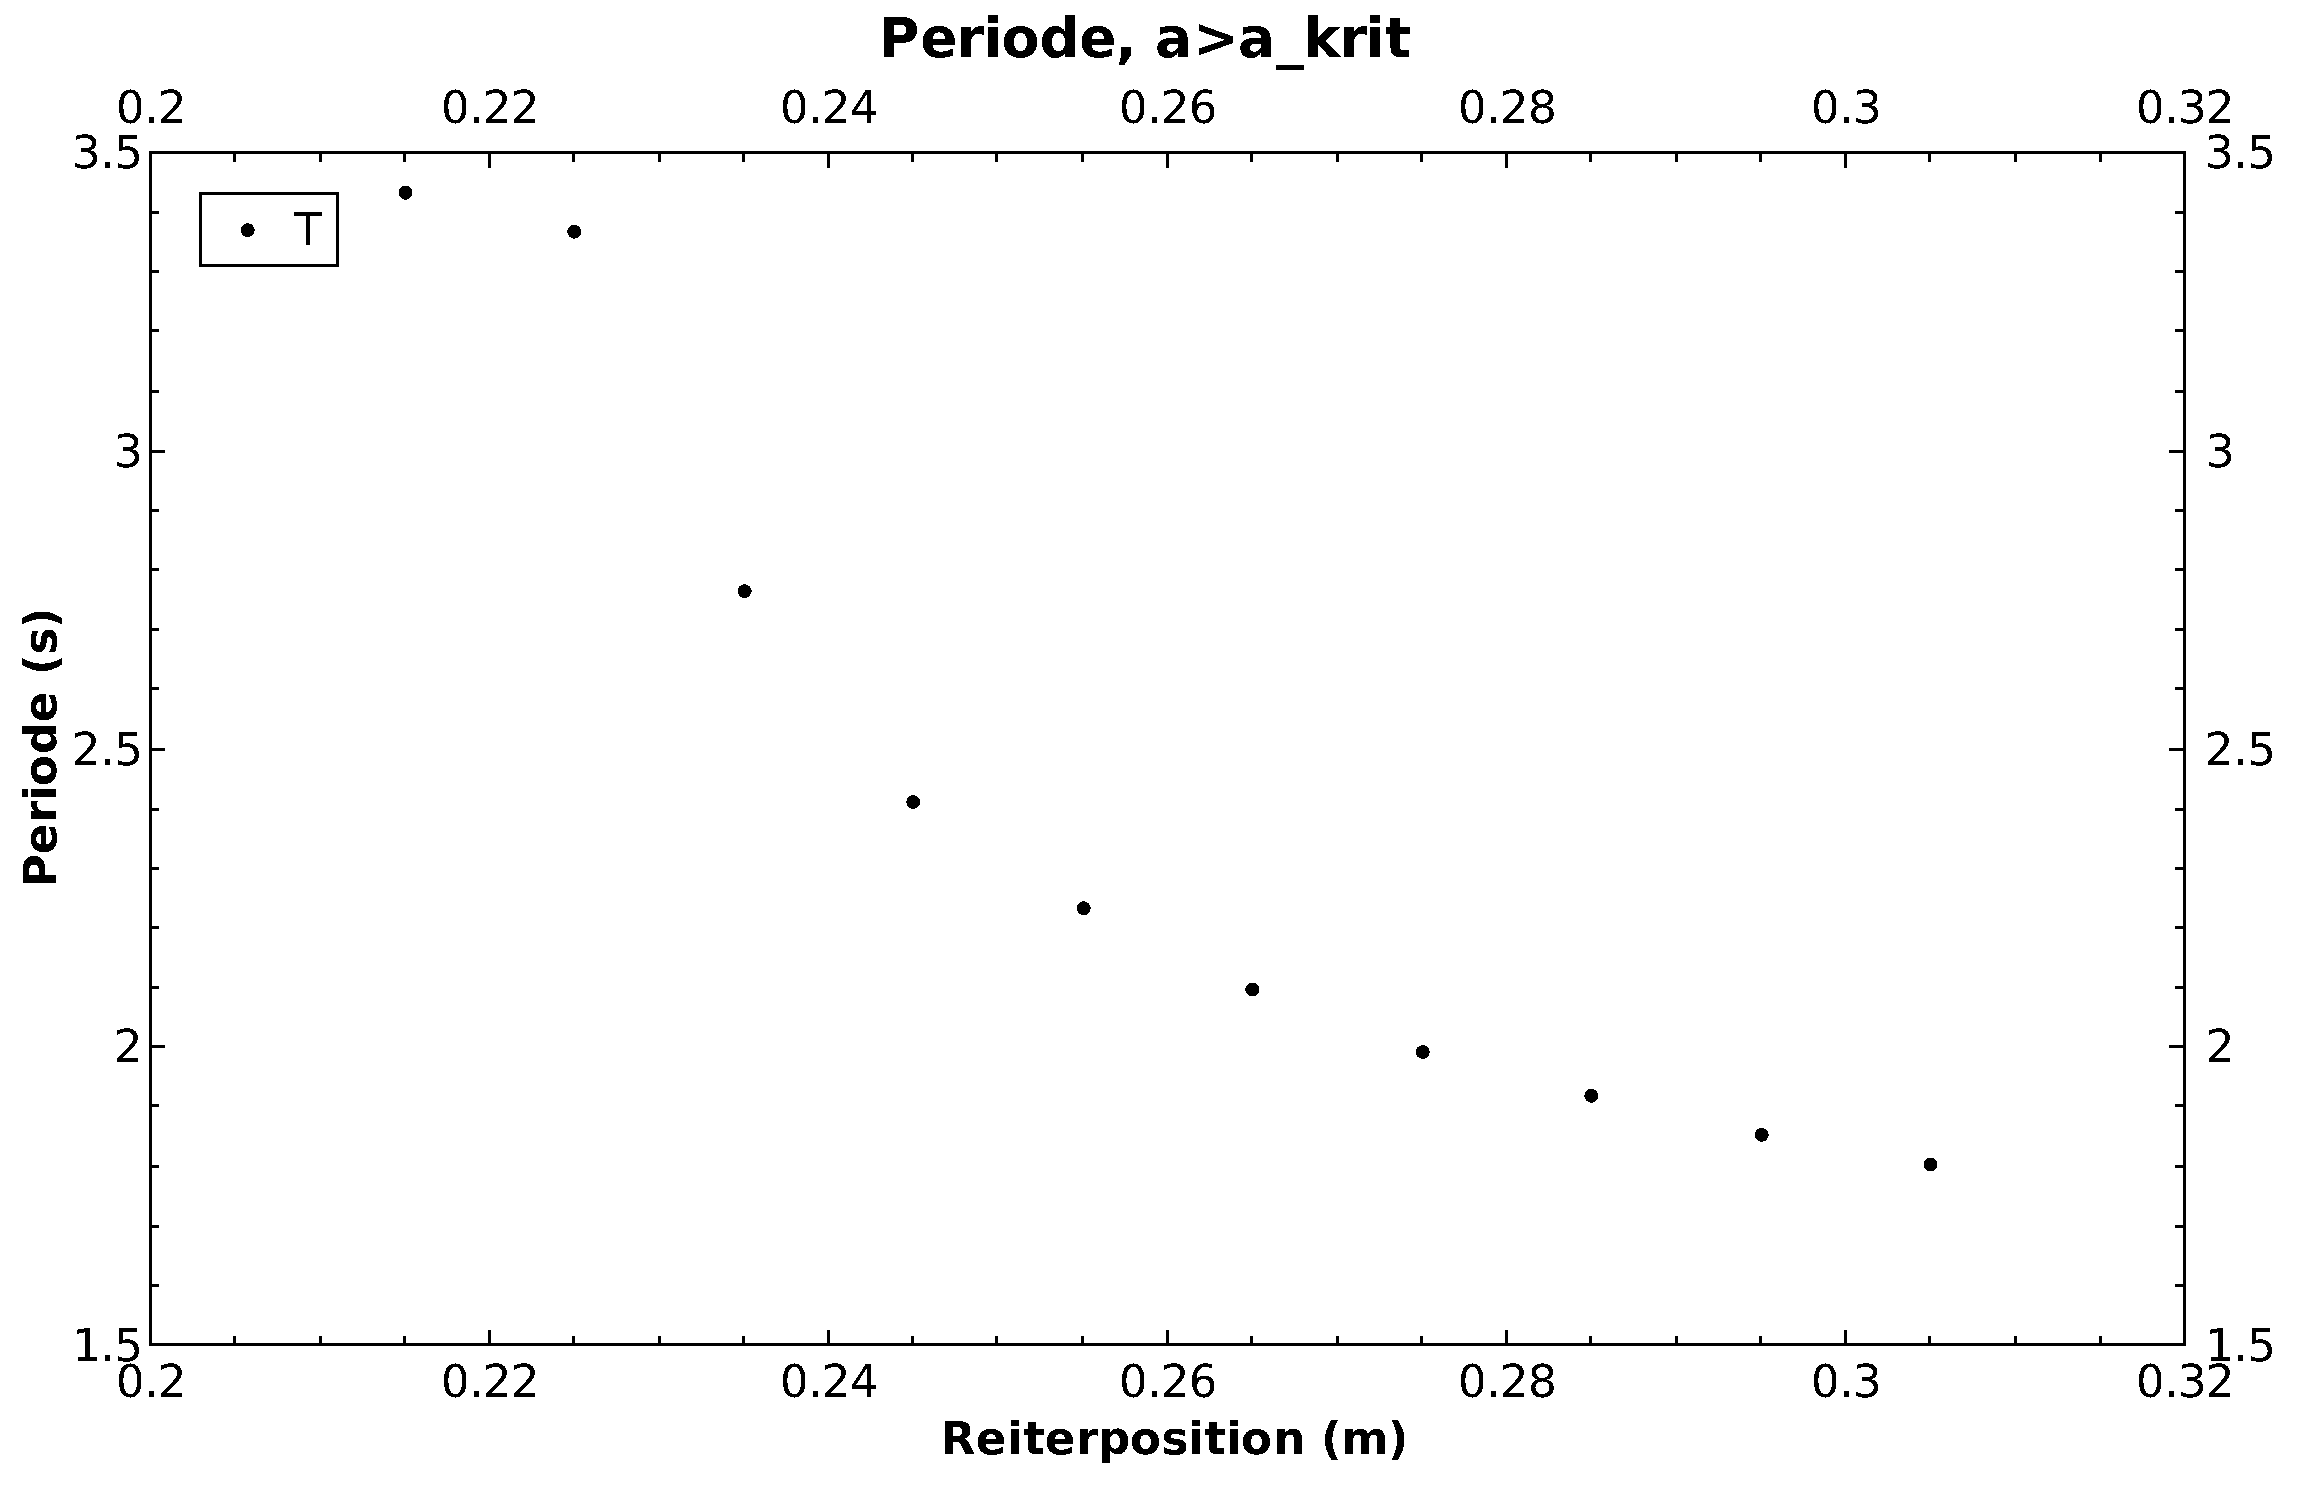
\includegraphics[width=\textwidth]{images/333b.pdf}
    \caption{%
        Periode in Abh\"angigkeit der Reiterposition f\"ur $a>a_{krit}$
    }
    \label{fig:333b}
\end{figure}



% **************************************************************************** %
\clearpage
\section{Fehlerrechnung}
\label{sec:fehlerrechnung}
% **************************************************************************** %
% ---------------------------------------------------------------------------- %
\subsection{Versuch 3.1 -- Spektra der R\"ohren, Analyse von LiF}
\label{subsec:error:spektra}
% ---------------------------------------------------------------------------- %

Zur Rekapitulation nochmals die mittels Regression bestimmten Nullpunktfehler:

\begin{table}[h!]
	\centering
	\small
    \caption{Nullpunktfehler aus Regression}
	\label{tab:nullpunktfehler:LiF}
	\begin{tabular}{lr}
		\toprule

        Anodenmaterial & Nullpunktfehler $\vartheta_0$ \\

        \midrule

        Kupfer &
        $\vartheta_0 = \SI{-0.72925 \pm 0.080931}{\degree}$ \\

        Eisen &
        $\vartheta_0 = \SI{-0.70575 \pm 0.023094}{\degree}$ \\

        Molybd\"an &
        $\vartheta_0 = \SI{-0.70555 \pm 0.068961}{\degree}$ \\

		\bottomrule
	\end{tabular}
\end{table}

Das Ziel ist nun die Bestimmung des Netzebenenabstandes mittels der folgenden Gleichung:

\begin{equation}
	\label{eq:braggLattice}
    d = \frac{n \cdot \lambda}{2 \cdot sin \left( \vartheta_n - \vartheta_0 \right)}
\end{equation}

Wobei  f\"ur  $\vartheta_n$  die   halben  Z\"ahlrohrwinkel  einzusetzen  sind
(abgelesen  aus   den  Messdaten)  und  f\"ur   $\lambda$  die  entsprechenden
Wellenl\"angen  f\"ur  die  charakteristischen Spektrallinien  des  jeweiligen
Anodenmaterials.

Dies liefert f\"ur  jeden Peak jeder Anode einen Wert  f\"ur $d$ (Bestimmt via
Matlab):

\begin{table}[h!]
	\centering
	\small
    \caption{Netzebenenabst\"ande zu den einzelnen Peaks}
	\label{tab:lattices:LiF}
	\begin{tabular}{llr}
		\toprule

        Anodenmaterial & Peak & Netzebenenabstand \\

        \midrule

        Kupfer 								&
		$\beta_1$ 							&
	    \SI{203.9}{\pico\meter}  \\

		&
		$\beta_2$							&
	    \SI{203.5}{\pico\meter}  \\

		&
		$\alpha_1$ &
 	    \SI{204.4}{\pico\meter} \\

		&
		$\alpha_2$ &
 	    \SI{203.3}{\pico\meter} \\

        Eisen &
		$\beta_1$ &
 	    \SI{203.6}{\pico\meter} \\

		&
		$\beta_2$ &
 	    \SI{202.1}{\pico\meter} \\

		&
		$\alpha_1$ &
 	    \SI{204.0}{\pico\meter} \\

		&
		$\alpha_2$ &
 	    \SI{201.9}{\pico\meter} \\

        Molybd\"an &
		$\beta_1$ &
 	    \SI{209.0}{\pico\meter} \\

		&
		$\beta_2$ &
 	    \SI{207.5}{\pico\meter} \\

		&
		$\alpha_1$ &
 	    \SI{205.8}{\pico\meter} \\

		&
		$\alpha_2$ &
 	    \SI{204.6}{\pico\meter} \\

		&
		$\alpha_3$ &
 	    \SI{205.1}{\pico\meter} \\

		\bottomrule
	\end{tabular}
\end{table}

Diese Werte k\"onnen nun gemittelt werden mittels der bekannten Formel:

\begin{equation*}
    \overline{x} = \frac{1}{N} \sum_{i=1}^{N}{x_i}
\end{equation*}

Und ihr Fehler bestimmt werden mittels der Formel:

\begin{equation*}
    s_{\overline{x}} = \sqrt{ \frac{\sum_{1}^{N}{(x_i-\overline{x})^2}}{N \cdot (N-1)}}
\end{equation*}

Da  Matlab   praktische  Befehle  zum  Verk\"urzen   dieser  Prozedur  bereits
integriert hat,  greifen wir darauf zur\"uck:  \code{mean(d)} und \code{std(d)
*  sqrt(1/length(d))},  wobei  \code{d}  der  Resultatvektor  mit  den  Werten
aus  Tabelle  \ref{tab:lattices:LiF}  ist.  \code{std(vector)}  berechnet  die
Standardabweichung der  Werte eines Vektors, \code{sqrt(1/length(d))}  ist der
Korrekturfaktor, um von der Standardabweichung auf den Fehler des Mittelwertes
der Werte des Vektors zu kommen.

Dies liefert f\"ur den Netzebenenabstand von LiF:

\begin{equation*}
    d_{LiF} = \SI{204.5 \pm 0.6}{\pico\meter}
\end{equation*}

Das  zugeh\"orige   Script  ist  in  Anhang   \ref{app:subsec:LiF}  auf  Seite
\pageref{app:subsec:LiF} zu finden.


% ---------------------------------------------------------------------------- %
\subsection{Versuch 3.3 -- Planck-Konstante}
\label{subsec:error:planck}
% ---------------------------------------------------------------------------- %

Die von  Hand gesch\"atzten Unsicherheiten  wurden zusammen mit dem  im ersten
Teil  des Versuches  bestimmten Nullplunktfehler  in die  Bragg'sche Gleichung
eingesetzt:
$$\lambda_{Error}  =  \frac{2  \cdot sin  \left(\vartheta_{n,Error}  -  \vartheta_0 \right)}{n}$$
und  in  Wellenl\"angen  konvertiert.

Das hierf\"ur benutzte Matlab-Script ist in Anhang \ref{app:subsec:planck} auf
Seite \pageref{app:subsec:planck} zu finden.

Anschliessend wurden die daraus berechneten Fehler in QtiPlot als Fehlerspalte
benutzt f\"ur einen gewichteten  Regressions-Plot.  F\"ur die Unsicherheit des
End-Resultates wurde  abschliessend die Unsicherheit  aus dem Fit  von QtiPlot
benutzt.


\clearpage
% ---------------------------------------------------------------------------- %
\subsection{Andere Kristalle}
\label{subsec:error:othercrystals}
% ---------------------------------------------------------------------------- %


Wie   bereits   erw\"ahnt,   wurde   f\"ur  jede   Spektrallinie   von   jedem
Kristall   der   zugeh\"orige   Netzebenenabstand  mittels   der   Bragg'schen
Gleichung  berechnet (in  Matlab). Die  erhaltenen Resultate  sind in  Tabelle
\ref{tab:results:spektra:otherCrystals} zu sehen.

\begin{table}[h!]
    \centering
    \small
    \caption{%
        Die f\"ur die vier Kristalle bestimmten Netzebenenabst\"ande und ihre
		Unsicherheiten.
    }
    \label{tab:results:spektra:otherCrystals}
    \begin{tabular}{lrrrrrrrr}
        \toprule
        &
        \multicolumn{2}{l}{Bergkristall}         &
        \multicolumn{2}{l}{Kalkspat}             &
        \multicolumn{2}{l}{Pyrit}                &
        \multicolumn{2}{l}{Synth. Quartz} \\
        \midrule

        &
        d ($\beta$)  &
        d ($\alpha$) &
        d ($\beta$)  &
        d ($\alpha$) &
        d ($\beta$)  &
        d ($\alpha$) &
        d ($\beta$)  &
        d ($\alpha$) \\

        \midrule


        n = 1              &
        \SI{402.6}{\pico\meter} &
        \SI{406.2}{\pico\meter} &
        \SI{282.7}{\pico\meter} &
        \SI{314.2}{\pico\meter} &
        \SI{331.6}{\pico\meter} &
        \SI{366.5}{\pico\meter} &
        \SI{352.6}{\pico\meter} &
        \SI{391.0}{\pico\meter} \\


        n = 2                   &
        \SI{415.6}{\pico\meter} & % n = 2 bergk
        \SI{415.5}{\pico\meter} & % n = 2 bergk
        \SI{652.8}{\pico\meter} & % n = 2 kalksp
        \SI{684.2}{\pico\meter} & % n = 2 kalksp
                                &
                                &
        \SI{785.4}{\pico\meter} & % n = 2 synth
        \SI{897.1}{\pico\meter} \\ % n = 2 synth

        n = 3                   &
        \SI{408.2}{\pico\meter} & % n = 3 bergk
        \SI{421.5}{\pico\meter} & % n = 3 bergk
                                &
                                &
                                &
                                &
                                &
                                \\

        n = 4                   &
        \SI{406.5}{\pico\meter} & % n = 4 bergk
        \SI{423.6}{\pico\meter} & % n = 4 bergk
                                &
                                &
                                &
                                &
                                &
                                \\

		\midrule

        MW             &
        \SI{408.2}{\pico\meter} &
        \SI{416.7}{\pico\meter} &
        \SI{302.0}{\pico\meter} &
        \SI{310.1}{\pico\meter} &
        \SI{269.8}{\pico\meter} &
        \SI{270.4}{\pico\meter} &
        \SI{251.4}{\pico\meter} &
        \SI{251.1}{\pico\meter} \\

        MW (ges.)      &
        \multicolumn{2}{c}{\SI{412.5}{\pico\meter}} &
        \multicolumn{2}{c}{\SI{306.1}{\pico\meter}} &
        \multicolumn{2}{c}{\SI{251.6}{\pico\meter}} &
        \multicolumn{2}{c}{\SI{270.1}{\pico\meter}} \\

		\midrule

        Fehler         &
         \SI{2.7}{\pico\meter} &
         \SI{3.9}{\pico\meter} &
        \SI{12.8}{\pico\meter} &
         \SI{3.5}{\pico\meter} &
         \SI{0}{\pico\meter} &
         \SI{0}{\pico\meter} &
         \SI{3.0}{\pico\meter} &
         \SI{3.2}{\pico\meter} \\

        Fehler (ges.)    &
        \multicolumn{2}{c}{\SI{2.7}{\pico\meter}} &
        \multicolumn{2}{c}{\SI{5.9}{\pico\meter}} &
        \multicolumn{2}{c}{\SI{0.3}{\pico\meter}} &
        \multicolumn{2}{c}{\SI{1.8}{\pico\meter}} \\

        \bottomrule
    \end{tabular}
\end{table}

\textbf{Anmerkungen:}

\begin{itemize}
	\item
        \textbf{Allgemein:} Die   Resultate  streuen   teilweise  merklich. Es
        dr\"angt  sich  der  Verdacht  auf,   dass  hier  eine  Korrektur  des
        Nullpunktfehlers w\"unschenswert w\"are, wie dies beim LiF-Kristall
		gemacht wurde.
	\item
        \textbf{Bergkristall:} Sieht eigentlich ganz  passabel aus, verglichen
        mit den anderen drei Kristallen.
	\item
        \textbf{Kalkspat:} Hier  sieht  man  einen markenten  Sprung  zwischen
        $n  = 1$  und  $n  = 2$. Ich  f\"uhre  dies  auf die  Kristallstruktur
        zur\"uck,  und  nicht  auf  einen  Mess-  oder  Rechenfehler. Kalkspat
        hat  keine  kubische,  sondern eine  rhombische  Einheitszelle  (siehe
        Anhang Versuchsanleitung). Daher k\"onnen  je nach Einstrahlungswinkel
        verschiedene  Abst\"ande  zwischen  Netzebenen auftreten  (nicht  alle
        Netzebenen unter allen Winkeln sind identisch.
	\item
        \textbf{Pyrit:} Hier  konnten  nur  bei   $n  =  1$  Peaks  detektiert
        werden. Die enorm  kleinen Unsicherheiten  sind daher also  nicht etwa
        das Resultat von hervorragender  Messpr\"azision, sondern das Ergebnis
        einer enorm kleinen Anzahl Messwerte.
	\item
        \textbf{Synthetischer  Quartz:} Auch hier  gelten wieder  die gleichen
        \"Uberlegungen wie beim Kalkspat bez\"uglich verschiedener m\"oglicher
        Netzebenen, nur  dass dieser  Kristall keine rhombische,  sondern eine
        auf Sechsecken aufbauende Gitterstruktur.
\end{itemize}

Das f\"ur  diese Berechnungen benutzte  Matlab-Script befinder sich  in Anhang \ref{app:subsec:others} ab Seite \pageref{app:subsec:others}.



% **************************************************************************** %
\clearpage
\section{Resultate und Diskussion}
\label{sec:results}
% **************************************************************************** %
Es gibt  drei Parameter  zu evaluieren: Das Massentr\"agheitsmoment  $I_0$ der
Apparatur ohne Reiter,  die Periodendauer $T_0$ f\"ur  kleine Auslenkungen und
die Federkonstante $k$. Die numerischen Resultate  f\"ur $I_0$ sind in Tabelle
\ref{tab:resultsI0}  zu  finden;  Abbildung  \ref{fig:resultsI0}  zeigt  einen
graphischen Vergleich der verschiedenen Methoden.

\begin{table}[h!]
    \centering
    \caption{Ergebnisse f\"ur $I_0$ via verschiedene Methoden}
    \label{tab:resultsI0}
    \begin{tabular}{p{70mm}r}
        \toprule
        Methode                                                                 & Resultat \\
        \midrule
        Versuch 3.1.1                                                           & \SI{12.03 \pm 0.02}{\gram\meter\squared} \\
        Versuch 3.1.2, Reiter als Punktmasse approximiert                       & \SI{11.4 \pm 0.4}{\gram\meter\squared} \\
        Versuch 3.1.2, Reiter als Zylinder modelliert                           & \SI{11.3 \pm 0.4}{\gram\meter\squared} \\
        Versuch 3.1.2, Reiter als Zylinder modelliert, eingeengter Fit-Bereich  & \SI{12.31 \pm 0.09}{\gram\meter\squared} \\
        Referenz Versuchsanleitung                                              & \SI{11.6}{\gram\meter\squared} \\
        \bottomrule
    \end{tabular}
\end{table}

\begin{figure}[ht!]
\centering
\begin{tikzpicture}
    \begin{axis}[
        width=.67\textwidth,
        height=.3\textwidth,
        %title = {Eisengehalt},
        xlabel = {$I_0$ ($\si{\kilo\gram\meter\squared}$)},
        %symbolic y coords = {ungewichtet,gewichtet, QtiPlot gewichtet},
        symbolic y coords = {Referenz Versuchsanleitung,Versuch 3.1.2 Zylinder 2,Versuch 3.1.2 Zylinder,Versuch 3.1.2 Punktmasse,Versuch 3.1.1},
    ]
    \addplot+[
        only marks,error bars/.cd,
        x dir=both,x explicit,
        error bar style={line width=0.5pt},
        ]
    coordinates {
        (1.20e-2,Versuch 3.1.1) +- (1.9e-5,0)
        (1.14e-2,Versuch 3.1.2 Punktmasse) +- (4e-4,0)
        (1.13e-2,Versuch 3.1.2 Zylinder) +- (4e-4,0)
        (1.23e-2,Versuch 3.1.2 Zylinder 2) +- (9e-5,0)
        (1.16e-2,Referenz Versuchsanleitung) +- (0,0)
    };
    \end{axis}
\end{tikzpicture}
\caption{graphische Darstellung der Ergebnisse zum f\"ur $I_0$}
\label{fig:resultsI0}
\end{figure}

F\"ur  die  Periode   $T_0$  beim  Schwerependel  ergaben   sich  zwei  Werte,
einer  f\"ur  den vollen  Messbereicht,  und  einer  aus  dem Fit  \"uber  den
eingeschr\"ankten  Wertebereich. Die  entsprechenden  Werte  sind  in  Tabelle
\ref{tab:resultsT0} respektive Abbildung \ref{fig:resultsT0} zu finden.

T\begin{table}[h!]
    \centering
    \caption{Ergebnisse f\"ur $T_0$ des Schwerependels}
    \label{tab:resultsT0}
    \begin{tabular}{p{70mm}r}
        \toprule
        Versuch                         & Resultat \\
        \midrule
        voller Messbereich              & \SI{1.403 \pm 0.006}{\second} \\
        eingeschr\"ankter Wertebereich  & \SI{1.419 \pm 0.002}{\second} \\
        \bottomrule
    \end{tabular}
\end{table}

\pgfplotsset{try min ticks=2}
\begin{figure}[ht!]
\centering
\begin{tikzpicture}
    \begin{axis}[
        width=.67\textwidth,
        height=.3\textwidth,
        %title = {Eisengehalt},
        xlabel = {$T_0$ ($\si{\second}$)},
        %symbolic y coords = {ungewichtet,gewichtet, QtiPlot gewichtet},
        symbolic y coords = {eingeschr\"ankter Wertebereich,voller Wertebereich},
    ]
    \addplot+[
        only marks,error bars/.cd,
        x dir=both,x explicit,
        error bar style={line width=0.5pt},
        ]
    coordinates {
        (1.40,voller Wertebereich) +- (0.006,0)
        (1.42,eingeschr\"ankter Wertebereich) +- (0.002,0)
    };
    \end{axis}
\end{tikzpicture}
\caption{graphische Darstellung der Ergebnisse zum f\"ur $T_0$ beim Schwerependel}
\label{fig:resultsT0}
\end{figure}

Zu   guter  Letzt   werden   in  Tabelle   \ref{tab:resultsk}  und   Abbildung
\ref{fig:resultsk} noch die Werte f\"ur die Federkonstante $k$ dargestellt und
verglichen.

\begin{table}[h!]
    \centering
    \caption{Ergebnisse f\"ur $k$ via verschiedene Methoden}
    \label{tab:resultsk}
    \begin{tabular}{p{70mm}r}
        \toprule
        Methode       & Resultat \\
        \midrule
        Versuch 3.3.1 & \SI{32.0   \pm  0.2}{\newton\per\meter} \\
        Versuch 3.3.2 & \SI{30.917 \pm  0.007}{\newton\per\meter} \\
        Versuch 3.3.3 & \SI{29.95 \pm  0.07}{\newton\per\meter} \\
        Referenzwert  & \SI{32.0}{\newton\per\meter} \\
        \bottomrule
    \end{tabular}
\end{table}

\pgfplotsset{try min ticks=4}
\begin{figure}[ht!]
\centering
\begin{tikzpicture}
    \begin{axis}[
        width=.67\textwidth,
        height=.3\textwidth,
        %title = {Eisengehalt},
        xlabel = {$k$ ($\si{\newton\per\meter}$)},
        symbolic y coords = {Referenzwert,Versuch 3.3.3,Versuch 3.3.2,Versuch 3.3.1},
    ]
    \addplot+[
        only marks,error bars/.cd,
        x dir=both,x explicit,
        error bar style={line width=0.5pt},
        ]
    coordinates {
        (32.0,Referenzwert) +- (0,0)
        (32.0,Versuch 3.3.1) +- (0.2,0)
        (30.9,Versuch 3.3.2) +- (0.007,0)
        (30.0,Versuch 3.3.3) +- (0.07,0)
    };
    \end{axis}
\end{tikzpicture}
\caption{graphische Darstellung der Ergebnisse zum f\"ur $k$}
\label{fig:resultsk}
\end{figure}


Alles   in  Allem   beurteile  ich   die  Ergebnisse   zufriedenstellent,  mit
Ausnahme  des  Fits  in  Abschnitt  \ref{subsubsec:kombiP:auslvar}  auf  Seite
\pageref{subsubsec:kombiP:auslvar},   welcher  aus   mir  bisher   unbekannten
Gr\"unden nicht wirklich stimmt (zumindest soweit ich dies beurteilen kann).



% **************************************************************************** %
\clearpage
\section*{Unterschrift}
\label{sec:signature}
% **************************************************************************** %
Ich best\"atige, dass ich diese Arbeit selbst\"andig gem\"ass Vorschriften des
Dozenten ausgef\"uhrt habe.

\vspace*{3em}

Raphael Frey:  \underline{\hspace{8cm}}

\vspace*{3em}

%Ort, Datum:  \underline{\hspace{5cm}},  \underline{\hspace{4cm}}
Oberentfelden, den \today.



% **************************************************************************** %
\clearpage
\begin{appendices}
    %\appendixpage
    %\addappheadtotoc
    %\appendix
    %\section{Anhang}
    \label{sec:appendix}
    % ************************************************************************ %
    % **************************************************************************** %
\section{Python-Code}
\label{app:python}
% **************************************************************************** %


% ---------------------------------------------------------------------------- $
\subsection{Laminare Str\"omung, symbolische Berechnungen}
\label{app:python:Qlaminar}
% ---------------------------------------------------------------------------- $
\lstinputlisting[style=python]{python/Qlaminar.py}


% ---------------------------------------------------------------------------- $
\clearpage
\subsection{Turbulente Str\"omung, symbolische Berechnungen}
\label{app:python:Qturb}
% ---------------------------------------------------------------------------- $
\lstinputlisting[style=python]{python/Qturb.py}


% ---------------------------------------------------------------------------- $
\clearpage
\subsection{Geschwindigkeit in Rohrmitte}
\label{app:python:rohrmitte}
% ---------------------------------------------------------------------------- $
\lstinputlisting[style=python]{python/rohrmitte.py}


% ---------------------------------------------------------------------------- $
\clearpage
\subsection{Str\"omungsprofile im laminaren Fall}
\label{app:python:laminar}
% ---------------------------------------------------------------------------- $
\lstinputlisting[style=python]{python/laminar.py}


% ---------------------------------------------------------------------------- $
\clearpage
\subsection{Str\"omungsprofile im turbulenten Fall}
\label{app:python:turbulent}
% ---------------------------------------------------------------------------- $
\lstinputlisting[style=python]{python/turbulent.py}


% ---------------------------------------------------------------------------- $
\clearpage
\subsection{Fehlerrechnung laminares Str\"omungsprofil}
\label{app:python:errorLaminar}
% ---------------------------------------------------------------------------- $
\lstinputlisting[style=python]{python/errorLaminar.py}

% ---------------------------------------------------------------------------- $
\clearpage
\subsection{Fehlerrechnung turbulentes Str\"omungsprofil}
\label{app:python:errorTurbulent}
% ---------------------------------------------------------------------------- $
\lstinputlisting[style=python]{python/errorTurbulent.py}


% ---------------------------------------------------------------------------- $
\clearpage
\subsection{Umrechnung Messposition zu Position in Messleitung}
\label{app:messposition}
% ---------------------------------------------------------------------------- $

Die  Laserstrahlen   kreuzten  sich   innerhalb  der  Messleitung   bei  einer
Positionsangabe   auf    der   Skala   f\"ur   die    Linse   $L_1$   zwischen
\SI{23}{\milli\meter}   und  \SI{53}{\milli\meter},   was  ein  Intervall  von
\SI{30}{\milli\meter} ergab. Aufgrund des unterschiedlichen Brechungsindex von
Luft Wasser ist dies zu erwarten (siehe Abbildung \ref{fig:lichtbrechung}).

Da   bekannt   ist,   dass   die  Messleitung   einen   Innendurchmesser   von
\SI{40}{\milli\meter}  hat,   wurden  die  Messpositionen  mit   ein  bisschen
Tabellenkalkulation von der Skala auf der Messvorrichtung auf eine Position in
der Messleitung umgerechnet:
\lstinputlisting[%
    basicstyle=\ttfamily\footnotesize\bfseries,
    xleftmargin=0.15\textwidth,
    ]{tables/scales.txt}

Es sei  hier noch  angemerkt, dass dieser  Effekt auf  die Dopplerverschiebung
keinen  Einfluss hat,  weshalb  sie f\"ur  die  Bestimmung des  Schnittwinkels
$\varphi$  in  Abschnitt \ref{subsec:varphi}  (Seite  \pageref{subsec:varphi})
nicht ber\"ucksichtigt wurde.

\vspace{0.5em}
\noindent\adjustbox{valign=t}{\begin{minipage}{0.40\textwidth}
    \captionof{figure}{%
        Verschiebung des  Schnittpunktes der Laserstrahlen in  der Messleitung
        aufgrund der unterschiedlichen Brechungsindizes von Luft und Wasser.
    }
    \label{fig:lichtbrechung}
\end{minipage}}
\adjustbox{valign=t}{\begin{minipage}{0.60\textwidth}
    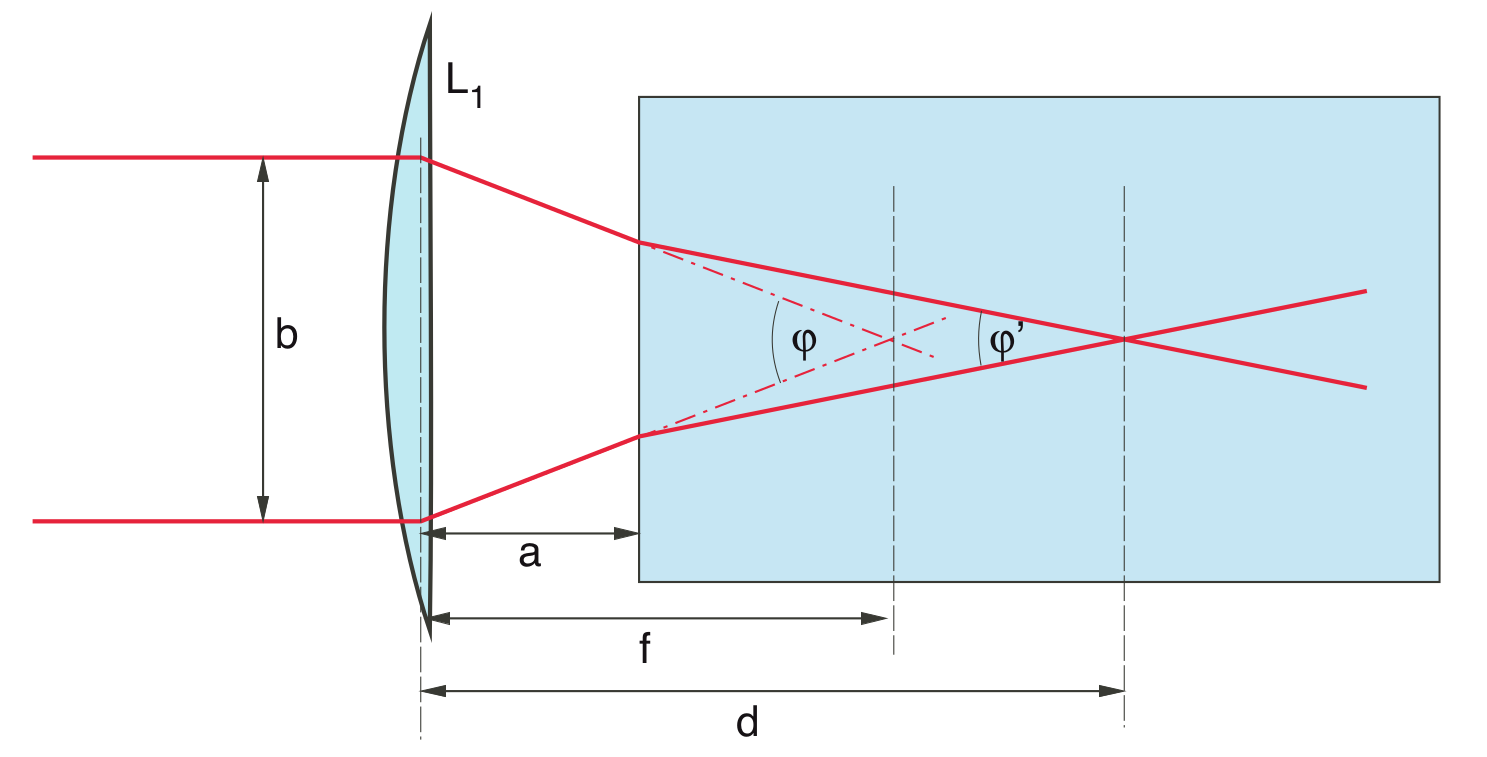
\includegraphics[width=\textwidth]{images/lichtbrechung.png}
\end{minipage}}


% ---------------------------------------------------------------------------- $
\clearpage
\section{Messprotokolle}
\label{app:messprotokolle}
% ---------------------------------------------------------------------------- $
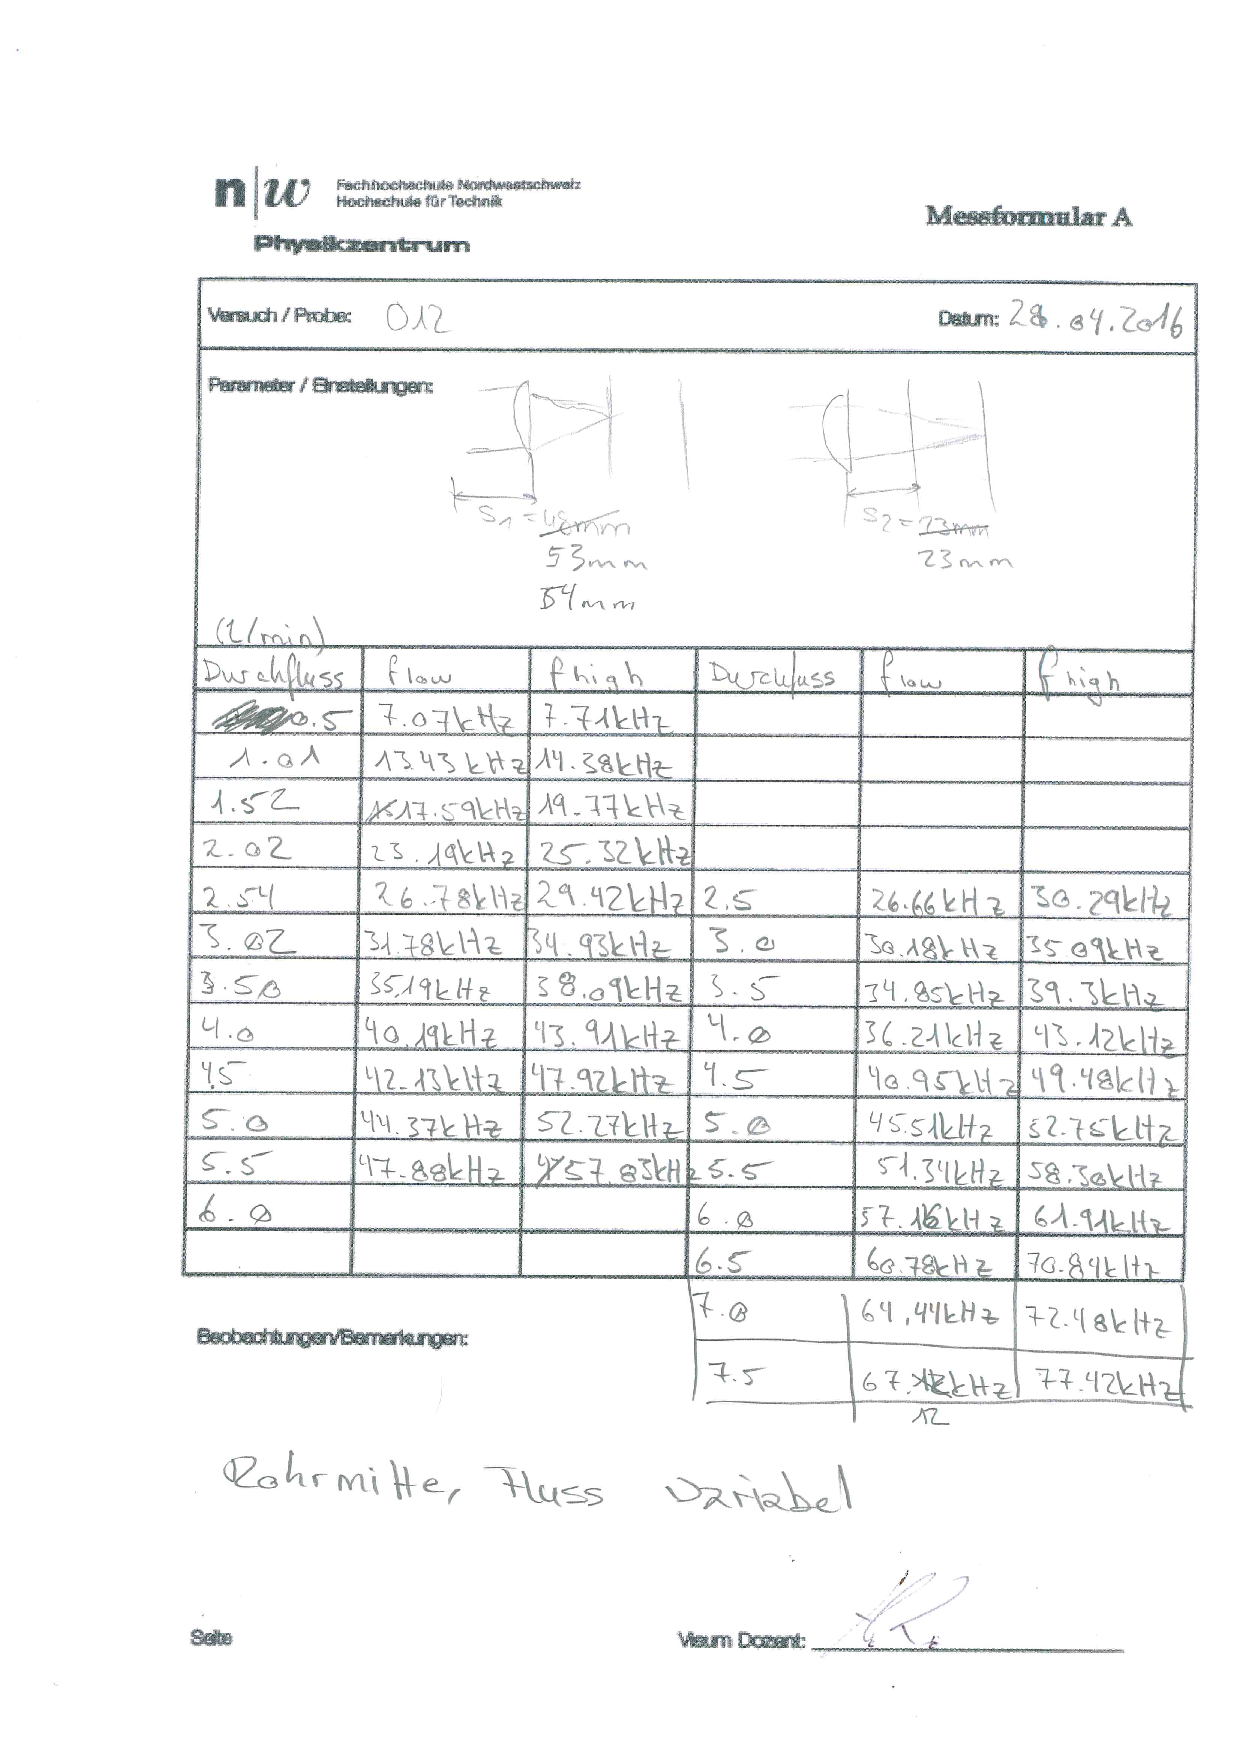
\includepdf[pages=-]{images/messprotokolle.pdf}

\end{appendices}

% **************************************************************************** %
\clearpage
\phantomsection
\addcontentsline{toc}{section}{\bibname}
\bibliography{bibliography/bibliography}{\bibliographystyle{bibliography/deIEEEtran.bst}}
% **************************************************************************** %
\end{document}
